        %%******************************************%%
        %%                                          %%
        %%        Modello di tesi di laurea         %%
        %%            di Andrea Giraldin            %%
        %%                                          %%
        %%             2 novembre 2012              %%
        %%                                          %%
        %%******************************************%%

\begin{document}
    \frontmatter
    \begin{titlepage}
    \begin{center}
        \begin{LARGE}
            \textbf{\myUni}\\
        \end{LARGE}

        \vspace{10pt}

        \begin{Large}
            \textsc{\myDepartment}\\
        \end{Large}

        \vspace{10pt}

        \begin{large}
            \textsc{\myFaculty}\\
        \end{large}

        \vspace{30pt}
        \begin{figure}[htbp]
            \centering
            
\includegraphics[height=6cm]{unipd-logo}
        \end{figure}
        \vspace{30pt}

        \begin{LARGE}
            \textbf{\myTitle}\\
        \end{LARGE}

        \vspace{10pt}

        \begin{large}
            \textsl{\myDegree}\\
        \end{large}

        \vspace{40pt}

        \begin{large}
            \begin{flushleft}
                \textit{Relatore}\\
                \vspace{5pt}
                \profTitle\ \myProf
            \end{flushleft}

            % You can tweak the spacing to have professor and student names on the same line
            % useful if the page is broken by a long thesis title and you need more space
            % \vspace{-52pt}

            \begin{flushright}
                \textit{Laureando}\\
                \vspace{5pt}
                \myName \\
                \vspace{5pt}
                \textit{Matricola} \myID
            \end{flushright}
        \end{large}

        \vspace{40pt}

        \line(1, 0){338} \\
        \begin{normalsize}
            \textsc{Anno Accademico \myAA}
        \end{normalsize}
    \end{center}
\end{titlepage}

    \clearpage
\phantomsection
\thispagestyle{empty}

\hfill
\vfill

\noindent\myName: \textit{\myTitle,}
\myDegree,
\textcopyright\ \myTime.

    %\cleardoublepage
\phantomsection
\thispagestyle{empty}
\pdfbookmark{Dedica}{Dedica}

\vspace*{3cm}

\begin{center}
    Lorem ipsum dolor sit amet, consectetuer adipiscing elit. \\ \medskip
    --- Oscar Wilde
\end{center}

\medskip

\begin{center}
    Dedicato a ...
\end{center}

    \cleardoublepage
\phantomsection
\pdfbookmark{Sommario}{Sommario}
\begingroup
\let\clearpage\relax
\let\cleardoublepage\relax
\let\cleardoublepage\relax

\chapter*{Sommario}

Il presente documento descrive il lavoro svolto durante il periodo di stage, della durata di circa trecento ore, dal laureando Pinco Pallino presso l'azienda Azienda S.p.A.
Gli obbiettivi da raggiungere erano molteplici.\\
In primo luogo era richiesto lo sviluppo di ...
In secondo luogo era richiesta l'implementazione di un ...
Tale framework permette di registrare gli eventi di un controllore programmabile, quali segnali applicati
Terzo ed ultimo obbiettivo era l'integrazione ...

%\vfill

%\selectlanguage{english}
%\pdfbookmark{Abstract}{Abstract}
%\chapter*{Abstract}

%\selectlanguage{italian}

\endgroup

\vfill

    \cleardoublepage
\phantomsection
\pdfbookmark{Ringraziamenti}{ringraziamenti}

\begin{flushright}
    {
    \slshape
    ``Le vent se lève!  Il faut tenter de vivre.''} \\
    \medskip
    --- Paul Valéry
\end{flushright}


\bigskip

\begingroup
\let\clearpage\relax
\let\cleardoublepage\relax
\let\cleardoublepage\relax

\chapter*{Ringraziamenti}

\noindent \textit{Innanzitutto, vorrei esprimere la mia gratitudine al Prof. \myProf, mio relatore, per l'aiuto e il sostegno fornitomi durante la stesura di questa tesi.\\
Senza il suo prezioso contributo, questo lavoro non sarebbe stato realizzabile.}\\

\noindent \textit{Desidero ringraziare di cuore i miei genitori per il loro amore incondizionato, il loro sostegno costante e per essere stati sempre al mio fianco, soprattutto nei momenti più difficili durante i miei anni di studio.}\\

\noindent \textit{Un ringraziamento speciale va a mio fratello, per essere stato una presenza costante ed un punto di riferimento insostituibile durante il nostro percorso universitario. \\
Condividere questa esperienza con lui ha reso ogni traguardo più gratificante e ogni sfida più facile da affrontare.}\\

\noindent \textit{Infine, vorrei esprimere la mia gratitudine a tutti i miei amici e amiche, con cui ho condiviso anni indimenticabili, ricchi di avventure, momenti di spensieratezza e incoraggiamento nei momenti più difficili.}\
\bigskip

\noindent\textit{\myLocation, \myTime}
\hfill \myName

\endgroup

    \cleardoublepage
\pdfbookmark{\contentsname}{tableofcontents}
\setcounter{tocdepth}{2}
\tableofcontents
%\markboth{\contentsname}{\contentsname}
\clearpage

\begingroup
    \let\clearpage\relax
    \let\cleardoublepage\relax
    \let\cleardoublepage\relax

    % Figures list
    \phantomsection
    \pdfbookmark{\listfigurename}{lof}
    \listoffigures

    \vspace*{8ex}

    % Tables list
    \phantomsection
    \pdfbookmark{\listtablename}{lot}
    \listoftables

    \vspace*{8ex}
\endgroup

\cleardoublepage

    \cleardoublepage

    \mainmatter
    \chapter{Contesto aziendale}
\label{cap:contesto-aziendale}

\section{Introduzione all'azienda}
\label{sez:introduzione-azienda}

Di cosa si occupa l'azienda, come è strutturata, quando è stata creata, ecc.\\
\section{Servizi e prodotti offerti}
\label{sez:servizi-prodotti-offerti}

Che servizi offre l'azienda (creazione web apps, creazione mobile apps, ecc.), quali prodotti offre, ecc.\\
\section{Way of working}
\label{sez:way-of-working}

\subsection{Metodologia di lavoro}
\label{sez:metodologia-lavoro}

Durante il mio periodo di \textit{stage} ho potuto sperimentare in prima persona la metodologia di lavoro adottata da \textbf{Zero12} per lo sviluppo dei progetti.\\
L'azienda utilizza una metodologia di sviluppo \textit{Agile}, utilizzando il \textit{framework} \textit{Scrum}, che permette di gestire progetti complessi e di portata variabile,
garantendo una maggiore flessibilità e adattabilità ai cambiamenti.\\
Ogni progetto viene diviso in \textit{sprint} di durata variabile, solitamente di una o due settimane, durante le quali vengono sviluppate le funzionalità concordate con il cliente.\\
Durante il mio \textit{stage} la lunghezza di ogni \textit{sprint} è stata di una settimana, per poter avere un \textit{feedback} più rapido sul lavoro svolto.\\
Ogni progetto viene gestito da un \textit{team} composto da un \textit{Product Owner}, uno \textit{Scrum Master} ed uno o più \textit{developer}, ognuno con un ruolo ben definito all'interno del progetto.\\

Il flusso che ogni progetto segue è il seguente:
\begin{itemize}
    \item \textbf{\textit{\gls{user-stories}}:} il \textit{Product Owner} definisce le funzionalità richieste dal cliente sotto forma di \textit{user stories}, brevi descrizioni delle funzionalità richieste dal cliente;
    Queste saranno poi inserite all'interno del \textit{\gls{product-backlog}}, ovvero la lista delle attività da svolgere.
    \item \textbf{\textit{Sprint Planning}:} all'inizio di ogni \textit{sprint} il \textit{team} si riunisce per pianificare le attività da svolgere durante la settimana, selezionando le \textit{\gls{user-stories}} da sviluppare, 
    in base alla loro priorità e alla loro complessità.
    \item \textbf{\textit{Daily Standup}:} ogni giorno il \textit{team} si riunisce per fare il punto della situazione, ognuno dei membri del \textit{team} riporta come procede il lavoro,
    cosa è stato fatto il giorno precedente e cosa si prevede di fare durante la giornata.
    \item \textbf{\textit{Sprint Review}:} alla fine di ogni \textit{sprint} il \textit{team} si riunisce con il cliente per mostrare le funzionalità sviluppate durante la settimana, controllando che il lavoro sia stato svolto efficientemente e 
    che soddisfi le aspettative del cliente.
    \item \textbf{\textit{Sprint Retrospective}:} alla fine di ogni \textit{sprint} il \textit{team} si riunisce per fare il punto della situazione dello \textit{sprint} appena terminato, 
    valutando il lavoro svolto e cercando miglioramenti per i prossimi \textit{sprint}.
\end{itemize}
\pagebreak

\subsection{Strumenti adottati}
\label{sez:strumenti-adottati}

\subsubsection{Strumenti organizzativi}
\label{sez:strumenti-organizzativi}

\noindent \textbf{Jira\\}

\noindent \textit{Jira} è un \gls{its} che permette la gestione delle attività di progetto in modo \textit{Agile}, fa parte della suite di prodotti di \textit{Atlassian}.\\
Un \gls{its} permette ai membri del team di visualizzare le attività assegnate, aggiornare lo stato di avanzamento e comunicare con gli altri membri del \textit{team} sul lavoro svolto. \\
Durante lo \textit{stage} l'ho utilizzato per la creazione di \textit{epic} e \textit{stories}, delle loro sotto \textit{task}, la pianificazione delle attività ed il tracciamento dei requisiti. \\
La {\hyperref[fig:jira-list-stories]{Figura 1.1}} mostra alcune delle \textit{stories} che ho creato durante l'attività di pianificazione.
\begin{figure}[H]
    \label{fig:jira-list-stories}
    \centering
    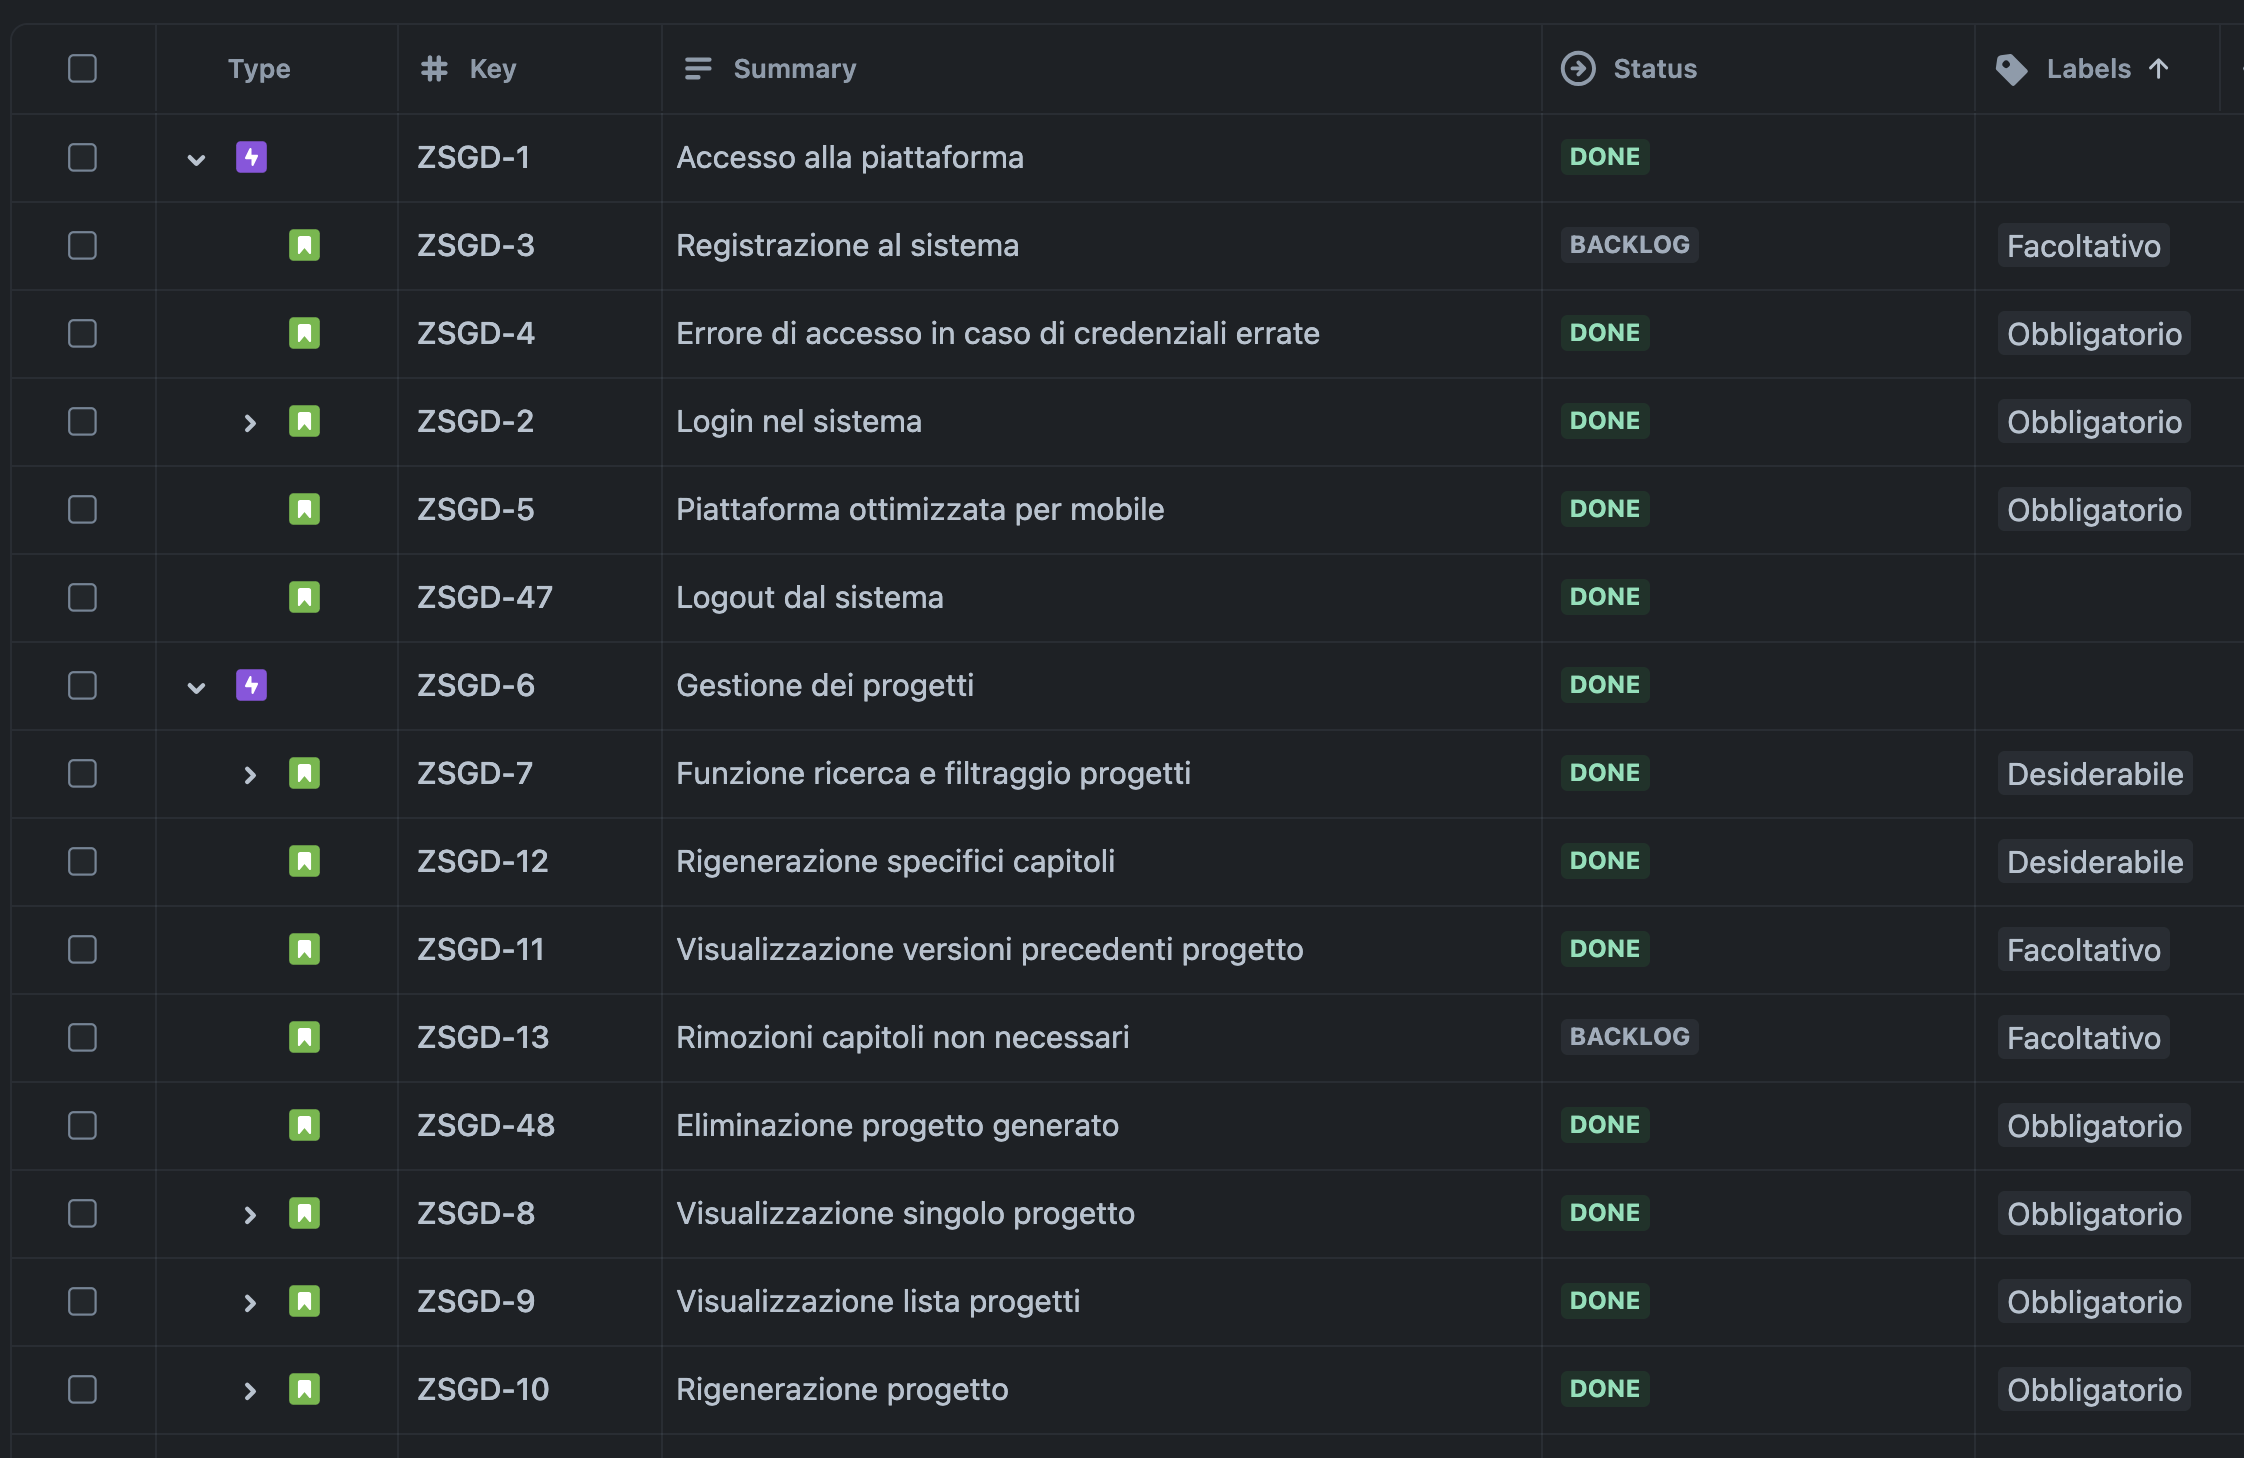
\includegraphics[scale=0.3]{strumenti/jira-list-stories.png}
    \caption{\textit{Jira} - Lista delle \textit{stories}}
\end{figure}

\noindent \textbf{Confluence\\}

\noindent \textit{Confluence} è un'applicazione di collaborazione che permette la creazione di documentazione in modo collaborativo tra i componenti di un \textit{team} di lavoro, fa parte della suite di prodotti di \textit{Atlassian}.\\
Durante lo \textit{stage} l'ho utilizzato per la creazione di documentazione relativa al progetto, come ad esempio la documentazione tecnica ed il documento di analisi progettuale.\\

\pagebreak
\noindent \textbf{Visual Studio Code\\}

\noindent \textit{Visual Studio Code} (da qui in poi \textit{VSCode}) è un \gls{ide} sviluppato da \textit{Microsoft}, che permette la scrittura del codice in diversi linguaggi di programmazione, è stato utilizzato per andare
a sviluppare tutto il codice del progetto utilizzando il linguaggio \textit{TypeScript}.\\
Un \gls{ide} permette di scrivere, testare ed effettuare il \textit{debugging} del codice in un'unica applicazione, fornendo strumenti per facilitare lo sviluppo del \textit{software}; \textit{VSCode} è uno degli \gls{ideg} più utilizzati.\\
La {\hyperref[fig:vscode]{Figura 1.2}} mostra l'interfaccia di sviluppo di \textit{VSCode}, il codice mostrato è relativo alla funzione di generazione di un progetto.

\begin{figure}[H]
    \label{fig:vscode}
    \centering
    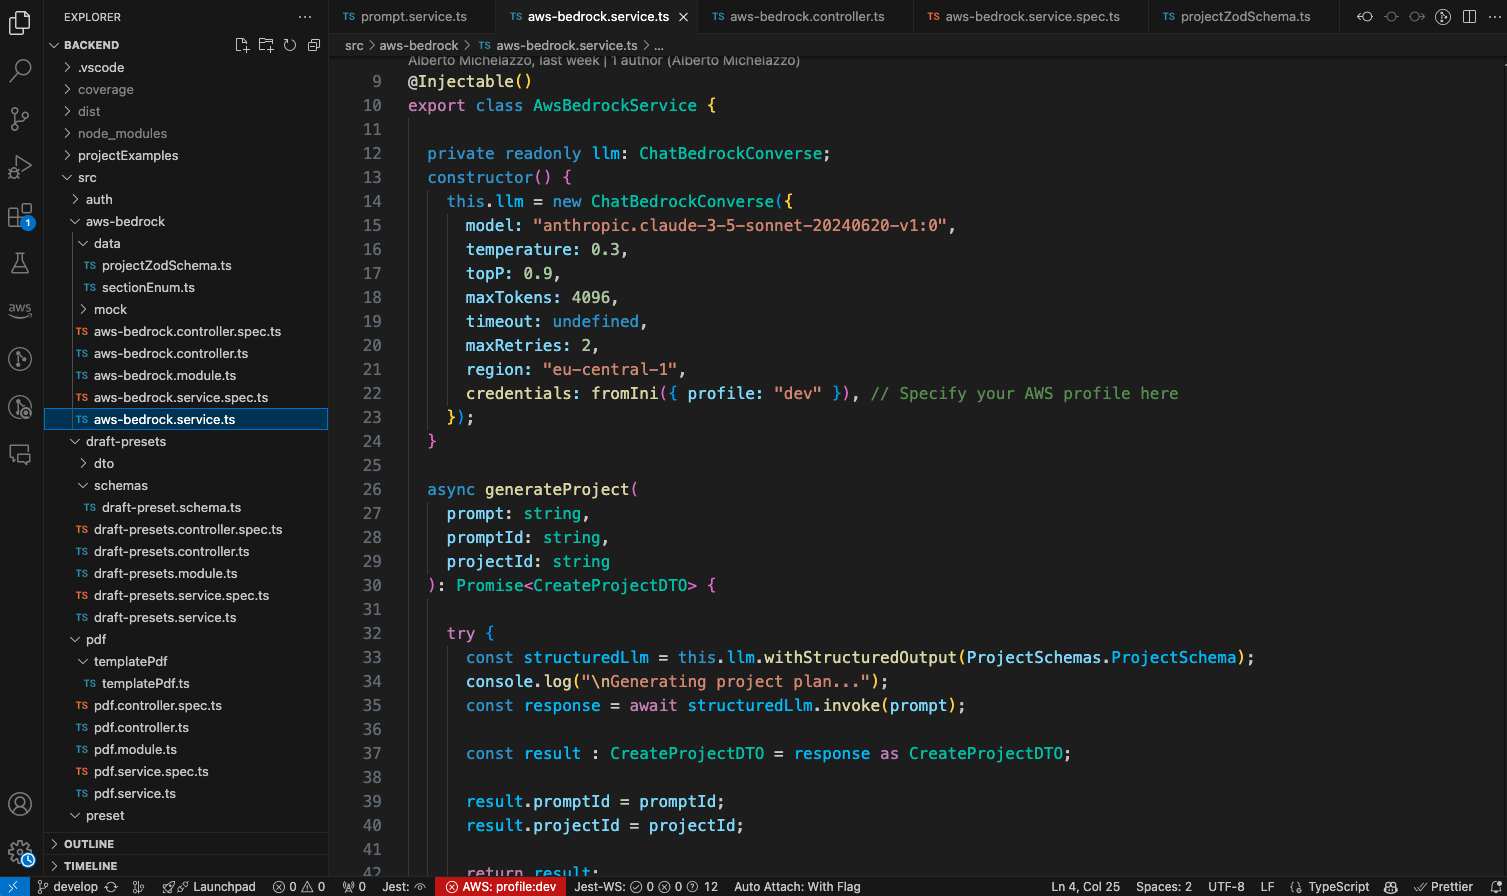
\includegraphics[scale=0.25]{strumenti/vscode.png}
    \caption{\textit{VSCode} - Interfaccia di sviluppo}
\end{figure}

\noindent \textbf{GitHub\\}

\noindent \textit{GitHub} è una piattaforma di \textit{hosting} per progetti \textit{software} che utilizzano il sistema di controllo di versione \textit{Git}.
Grazie a questa piattaforma è possibile andare a creare \textit{repositories} per il proprio progetto, permettendo la collaborazione tra i membri del \textit{team} ed il tracciamento delle modifiche effettuate. \\
È inoltre possibile andare a suddividere il progetto in \gls{branch}, per andare a sviluppare le funzionalità tramite cosidetti \textit{feature branch}.\\
Un \gls{branch} è una copia del codice principale del progetto, che permette di sviluppare nuove funzionalità senza influenzare il codice principale.\\
Terminata la codifica di una \textit{feature}, è possibile effettuare una \gls{pr} per andare ad unire il codice sviluppato con il \gls{branch} principale, dopo la revisione da parte di un collega.\\
Una \gls{pr} permette di discutere delle modifiche effettuate, garantire che il codice sia conforme alle \textit{best practices} del progetto e che non siano presenti errori.\\
La {\hyperref[fig:github]{Figura 1.3}} mostra una delle \textit{repositories} che ho creato per il progetto.

\begin{figure}[H]
    \label{fig:github} 
    \centering
    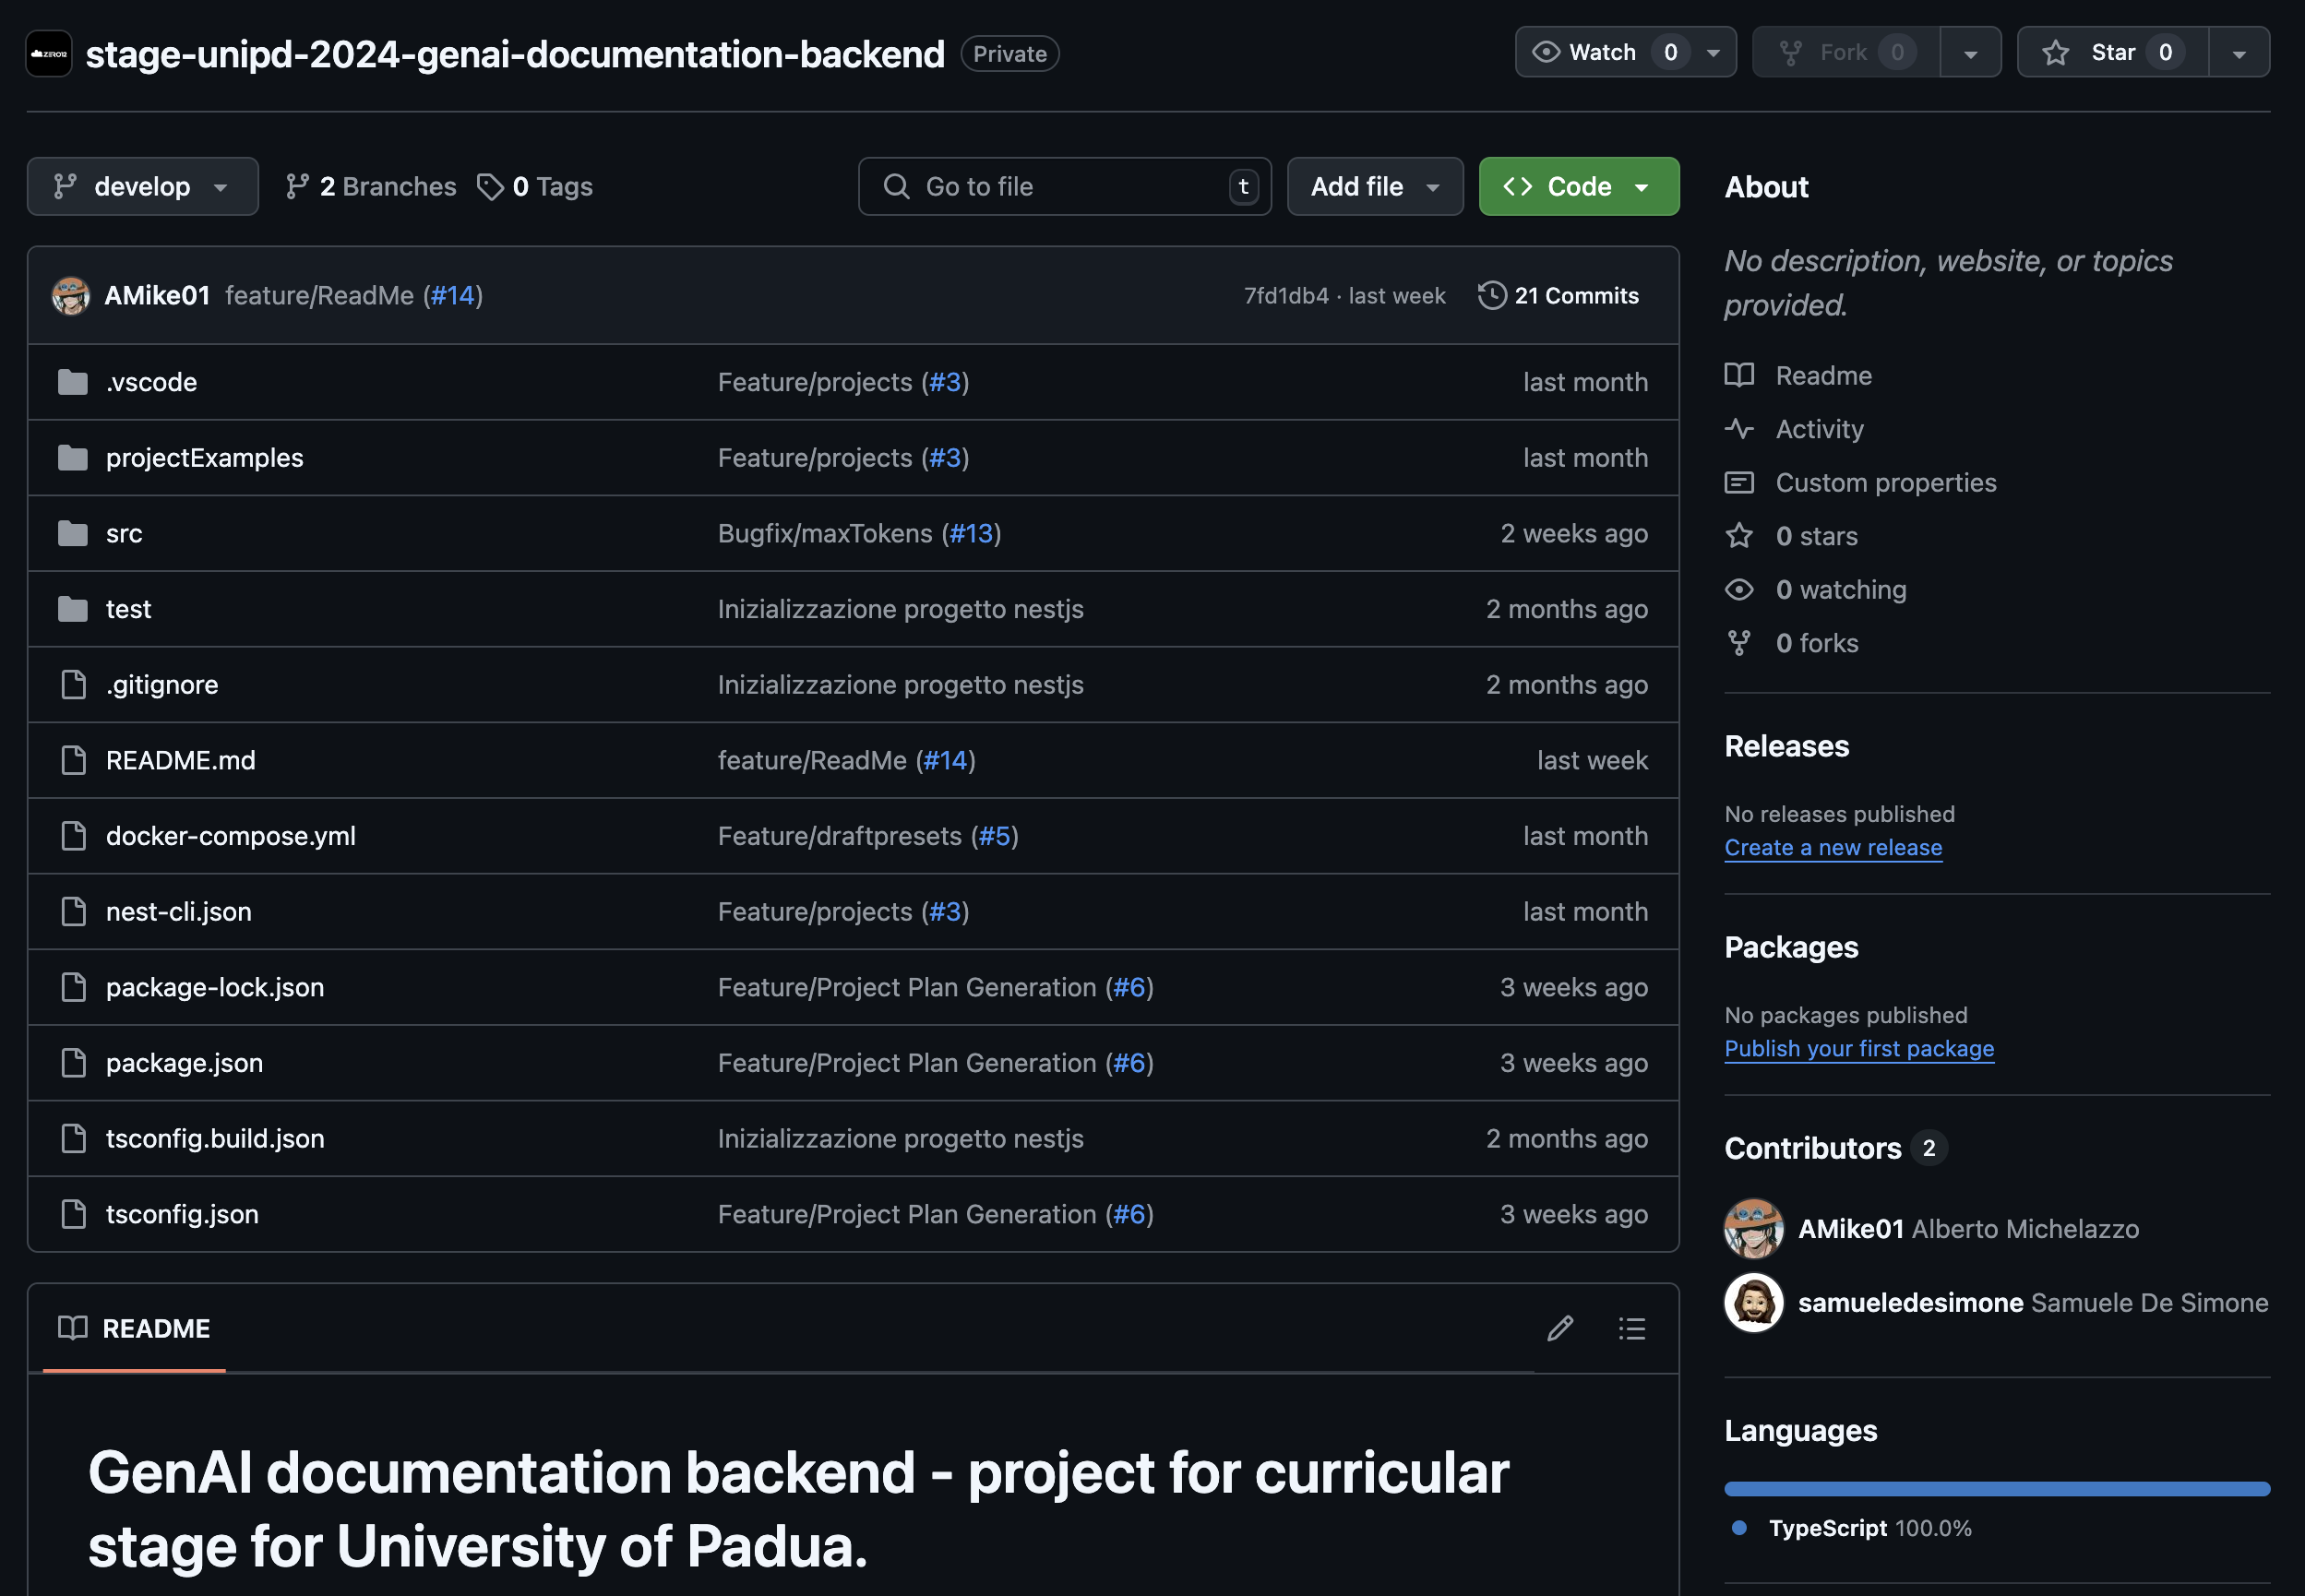
\includegraphics[scale=0.3]{strumenti/github-repo.png}
    \caption{\textit{GitHub} - Una delle \textit{repositories} create}
\end{figure}

\pagebreak

\subsubsection{Strumenti di comunicazione}
\label{sez:strumenti-comunicazione}

\noindent \textbf{Slack\\}

\noindent \textit{Slack} è un'applicazione di messaggistica istantanea che permette di comunicare con i propri colleghi in ambito aziendale. \\
Tramite la creazione di specifici canali è possibile organizzare le conversazioni per progetto, permettendo una comunicazione più efficace tra i membri del \textit{team}.\\
Come si può vedere nella {\hyperref[fig:slack]{Figura 1.4}}, nel caso del mio \textit{stage} è stato creato un canale dedicato al mio progetto, insieme al mio tutor ed ad un'altra figura aziendale, 
per poter comunicare in modo diretto e veloce in caso di problematiche o dubbi durante lo sviluppo.

\begin{figure}[H]
    \label{fig:slack} 
    \centering
    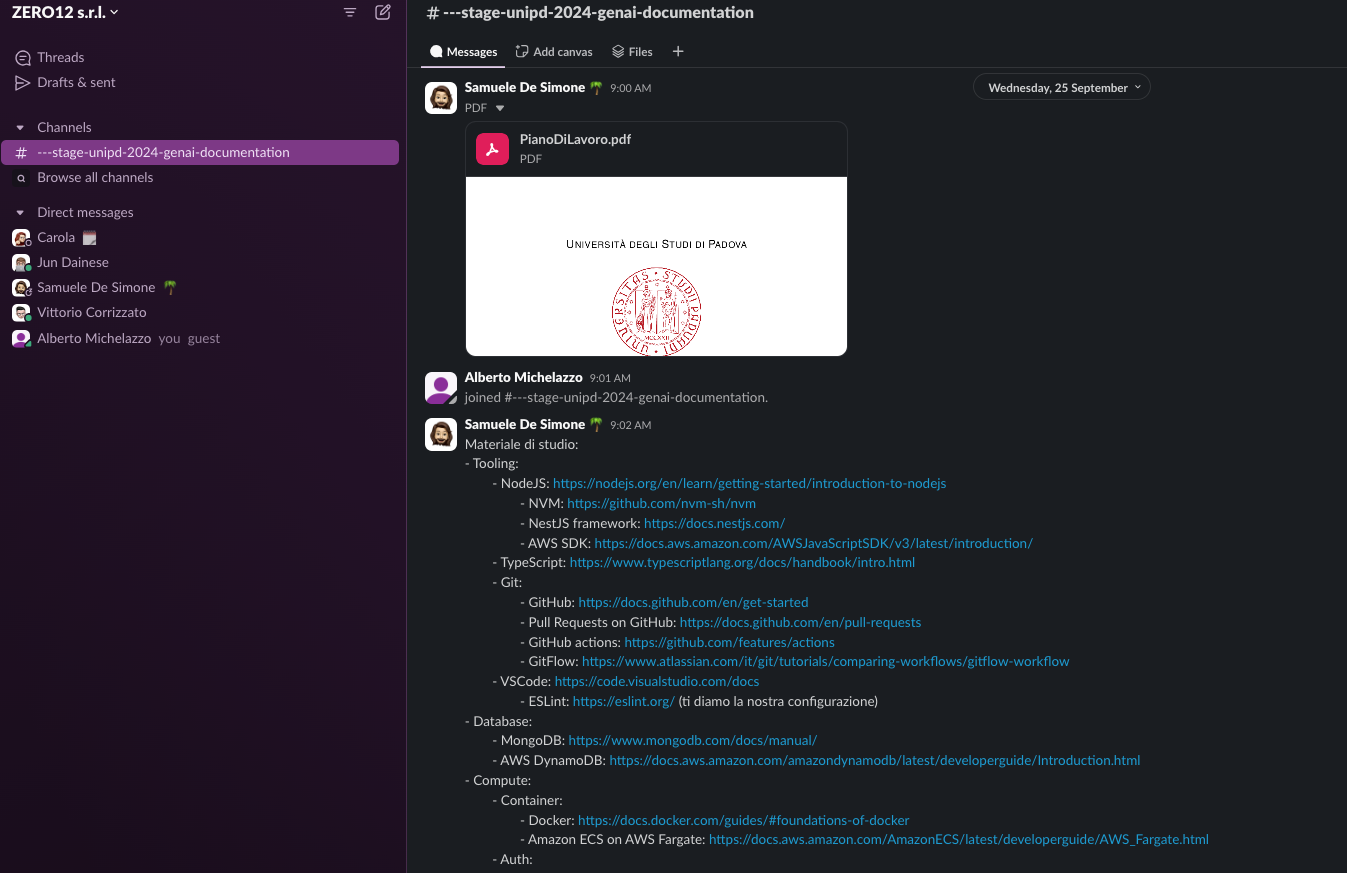
\includegraphics[scale=0.25]{strumenti/slack.png}
    \caption{\textit{Slack} - Canale dedicato al progetto}
\end{figure}

\noindent \textbf{Microsoft Teams\\}

\noindent \textit{Microsoft Teams} è un'applicazione di collaborazione che permette la comunicazione tra i membri del \textit{team}, la condivisione di \textit{file} e la gestione di riunioni.\\
Durante il mio \textit{stage} l'ho utilizzato per la gestione delle riunioni settimanali con il tutor aziendale, per discutere dello stato di avanzamento del progetto e per ricevere \textit{feedback} sul lavoro svolto, quando
non era possibile effettuare un incontro di persona.

\pagebreak
\section{Tecnologie utilizzate}
\label{sez:tecnologie-utilizzate}

\subsection{Tecnologie di sviluppo}
\label{sez:tecnologie-sviluppo}

\subsubsection{HTML}

Linguaggio di markup standard utilizzato per creazione di pagine \textit{web}.
Permette di strutturare i contenuti di una pagina \textit{web}, andando a definire la disposizione di testo, immagini, link, tabelle, ecc.

\subsubsection{CSS}
Linguaggio di stile utilizzato per descrivere l’aspetto e la formattazione dei componenti di una pagina \textit{web}.

\subsubsection{TypeScript}

“Superset” di \textit{JavaScript}, che va ad aggiungere funzionalità e tipizzazione statica al linguaggio; 
tramite l’utilizzo di un compilatore questo viene tradotto in \textit{JavaScript} che può essere poi eseguito dai \textit{browser}.

\subsubsection{React}
Un \textit{framework} sviluppato da Meta per la creazione di interfacce \textit{web}dinamiche, permette di creare \gls{spa} tramite dei componenti riutilizzabili realizzati in file \textit{JavaScript} (.jsx) o \textit{TypeScript} (.tsx).

\subsubsection{Material UI}

Una libreria di componenti \textit{React} che implementa il \textit{Material Design}, uno stile di design sviluppato da Google.\\
Questa libreria offre un set di componenti predefiniti e pronti all’uso, che è possibile andare a personalizzare in base alle proprie esigenze.

\subsubsection{Axios}

Una libreria \textit{JavaScript} che semplifica la comunicazione tra frontend e backend, consentendo di effettuare richieste \gls{http} (GET, POST, PUT, DELETE, ecc.) in modo efficiente e personalizzabile. \\
Offre supporto per \textit{Promises}, gestione avanzata degli errori e configurazioni flessibili per adattarsi a diverse esigenze.

\subsubsection{Zod}

Una libreria \textit{TypeScript} per la validazione ed il \textit{parsing} di dati, permette di definire degli schema per strutturare e convalidare oggetti, stringhe, \textit{array}, ecc.
È possibile utilizzarla per effettuare validazioni dei dati in ingresso e in uscita dalle \gls{api}.
\subsubsection{Styled Components}

Una libreria che permette di scrivere stili CSS all’interno dei componenti \textit{React}, è possibile andare a creare stili personalizzati per ogni componente \textit{React}, andando a rendere il codice più leggibile e manutenibile.

\begin{figure}[H]
    \label{fig:styled-components}
    \centering
    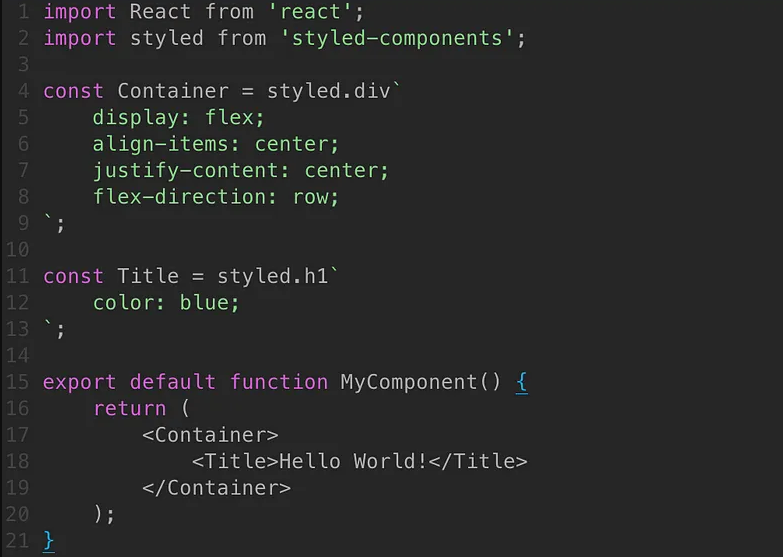
\includegraphics[scale=0.25]{tecnologie/styled-component.png}
    \caption{Esempio di utilizzo di \textit{Styled Components}}
    \cite{site:medium}
\end{figure}

\subsubsection{Vite}

Uno strumento di sviluppo utilizzato per inizializzare e configurare rapidamente il \gls{frontend} di un progetto, semplificando l'inizializzazione e ottimizzando l'esperienza di sviluppo.\\
È possibile utilizzarlo con vari \textit{framework} \gls{frontend} come ad esempio \textit{React}.

\subsubsection{React-PDF}

Libreria utilizzata per il \textit{rendering} di documenti PDF all’interno di pagine create in \textit{React}.
Consente di visualizzare, navigare ed interagire con i file PDF.

\subsubsection{Node.js}

Un ambiente di \textit{runtime JavaScript} basato sul motore V8 di \textit{Chrome}, utilizzato per eseguire codice lato \textit{server}. 
Consente di sviluppare applicazioni scalabili e ad alte prestazioni, grazie al modello asincrono e orientato agli eventi.

\subsubsection{NestJS}

Un \textit{framework} \gls{backend} moderno e robusto basato su \textit{Node.js}, progettato per creare applicazioni \textit{server} scalabili ed efficienti.
Ideale per costruire \textit{API RESTful, GraphQL} e applicazioni in tempo reale, grazie al supporto nativo per \textit{middleware}, guardie, filtri e \textit{interceptor}.
\pagebreak
\subsubsection{MongoDB}

Un \textit{database NoSQL} potente e flessibile progettato per la gestione di dati sotto forma di documenti \textit{JSON-like}. 
È ideale per applicazioni moderne grazie alla sua scalabilità orizzontale, alla capacità di gestire grandi volumi di dati non strutturati e alla facilità di integrazione con diverse tecnologie.

\begin{figure}[H]
    \label{fig:sql-nosql}
    \centering
    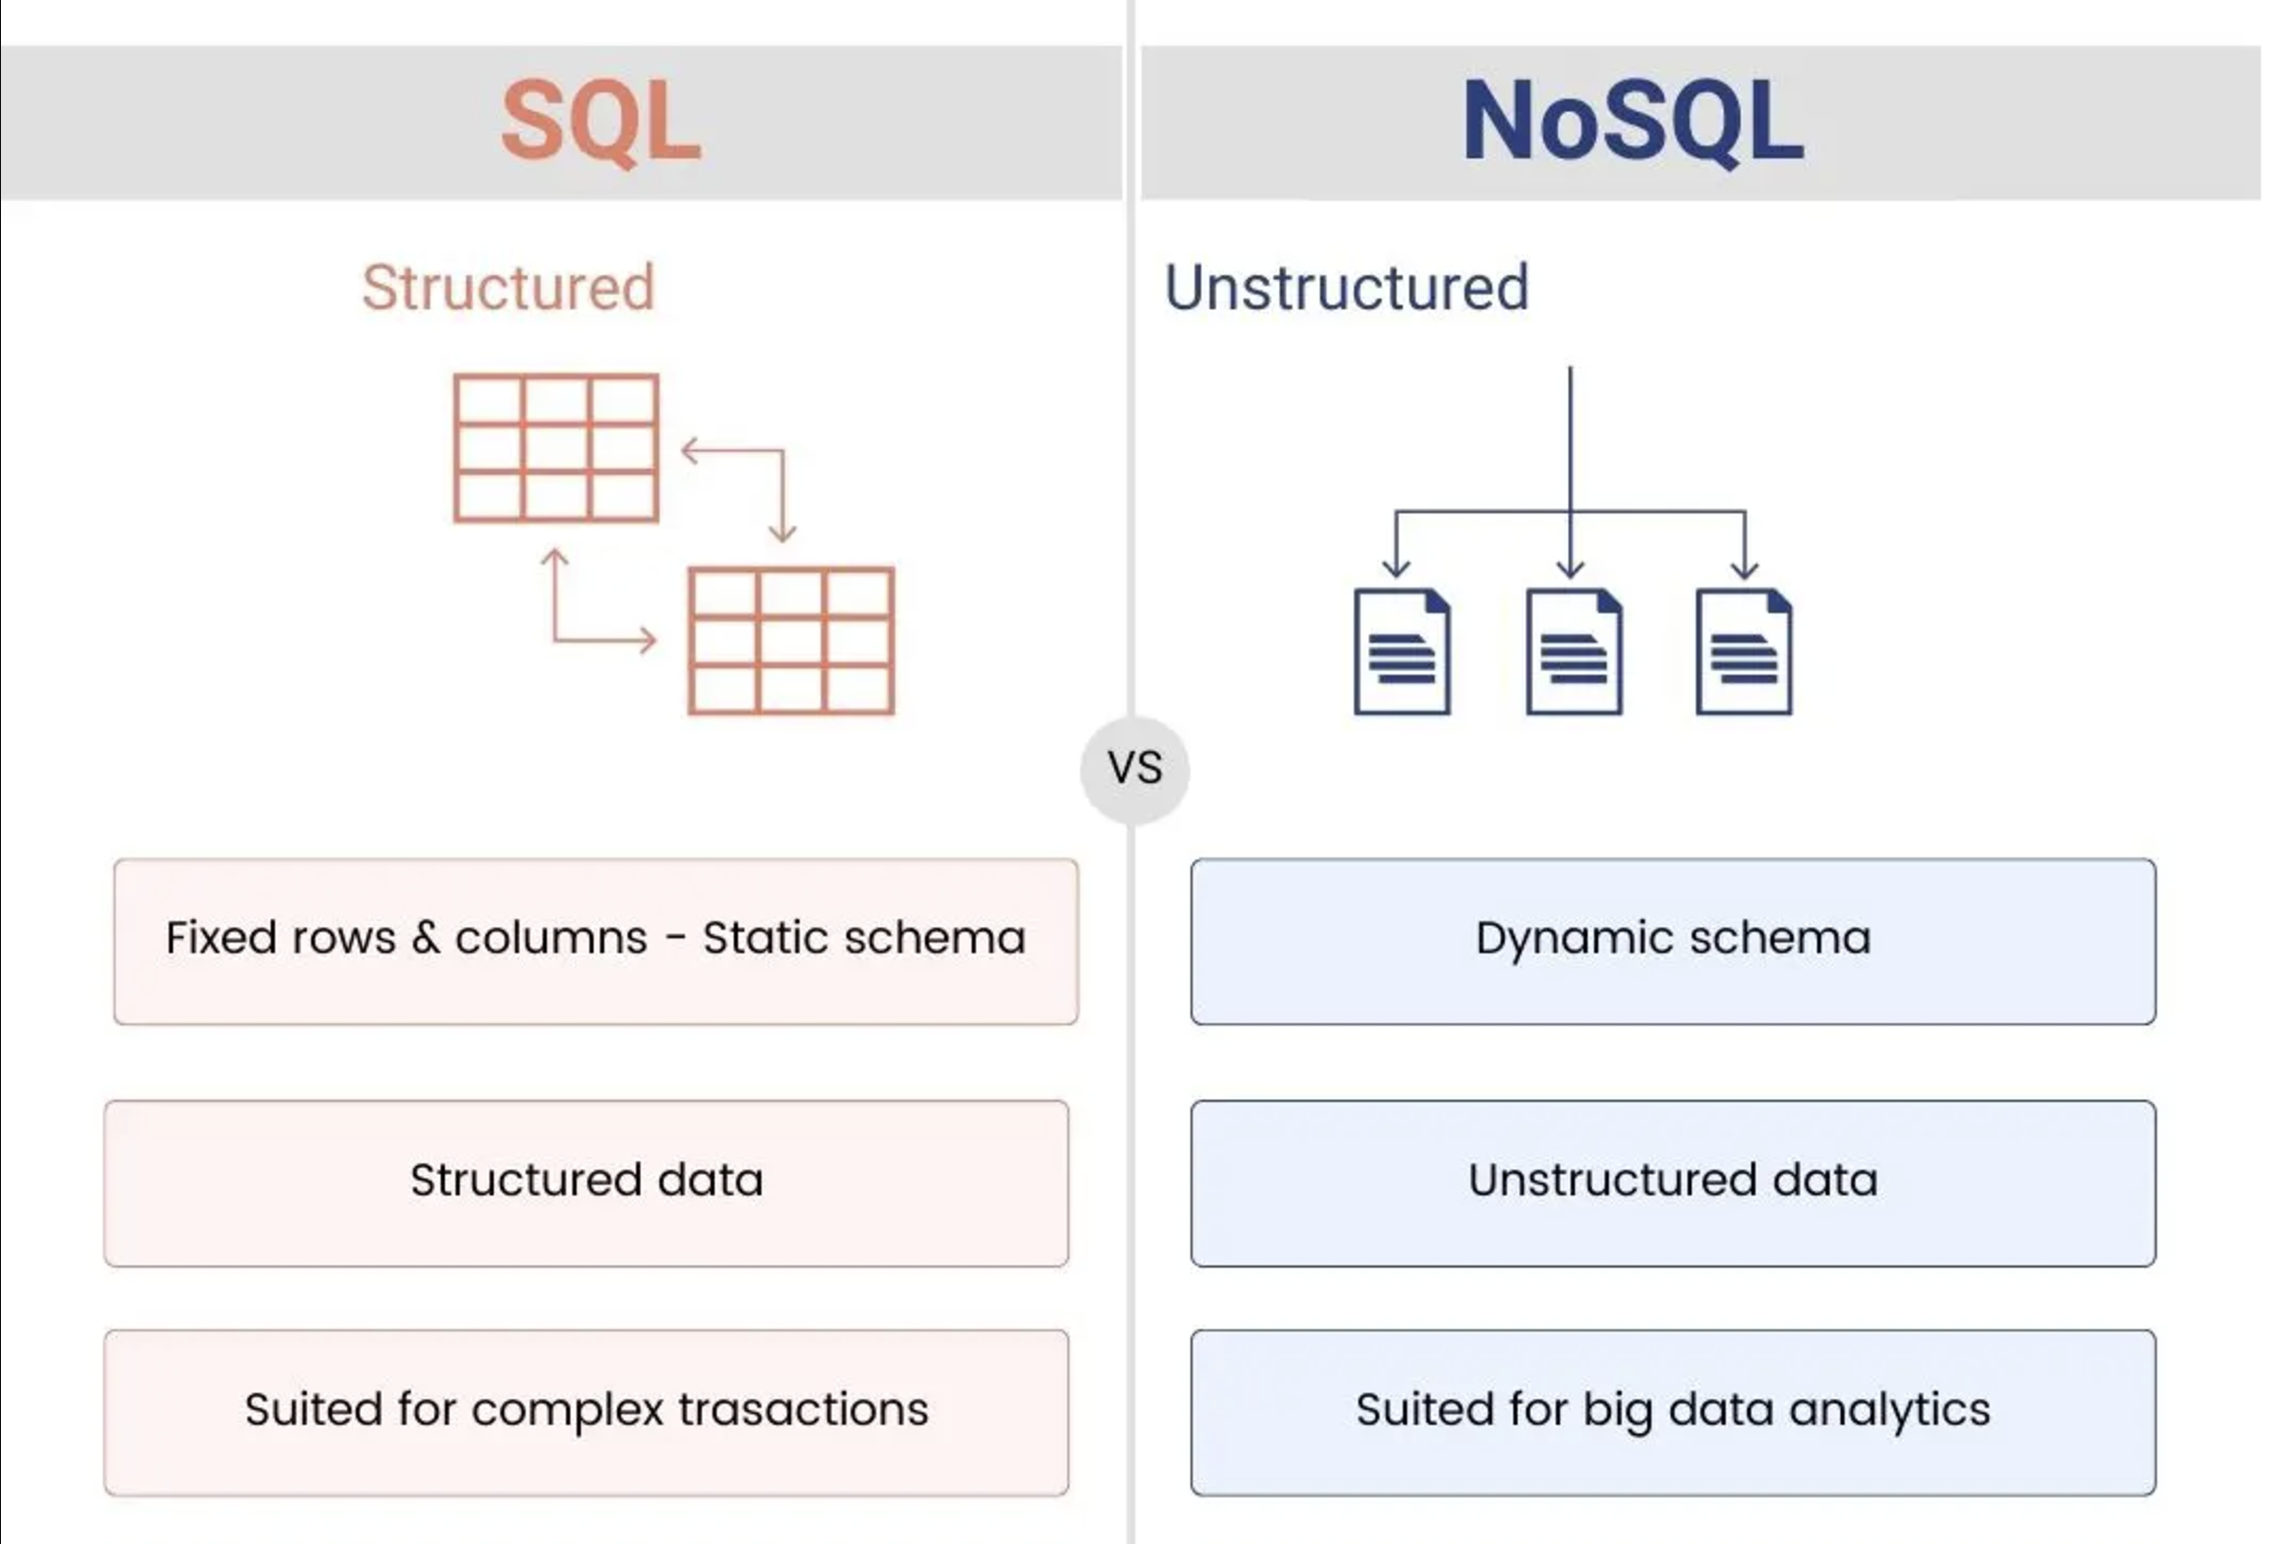
\includegraphics[scale=0.2]{tecnologie/sql-nosql.png}
    \caption{Principali differenze tra un \textit{database SQL} e un \textit{database NoSQL}}
\end{figure}

\subsubsection{Mongoose}

Un \gls{odm} per \textit{Node.js}, utilizzato per semplificare il collegamento tra \textit{NestJS} e \textit{MongoDB}. Consente di definire schemi per i dati, applicare validazioni, \textit{middleware} e trasformazioni direttamente a livello di modello. \\
\textit{Mongoose} offre un'API intuitiva per interagire con \textit{MongoDB}, supportando operazioni complesse come popolamenti, \textit{query} avanzate e gestione delle relazioni tra documenti. 

\subsubsection{LangChain}

Un \textit{framework} avanzato per lo sviluppo di applicazioni che utilizzano \gls{llm}. 
\textit{LangChain} semplifica la gestione delle chiamate \gls{api} ai modelli di linguaggio, offrendo strumenti per orchestrare flussi complessi, integrare memoria e combinare più modelli o fonti di dati.

\begin{figure}[H]
    \label{fig:langchain-usecases}
    \centering
    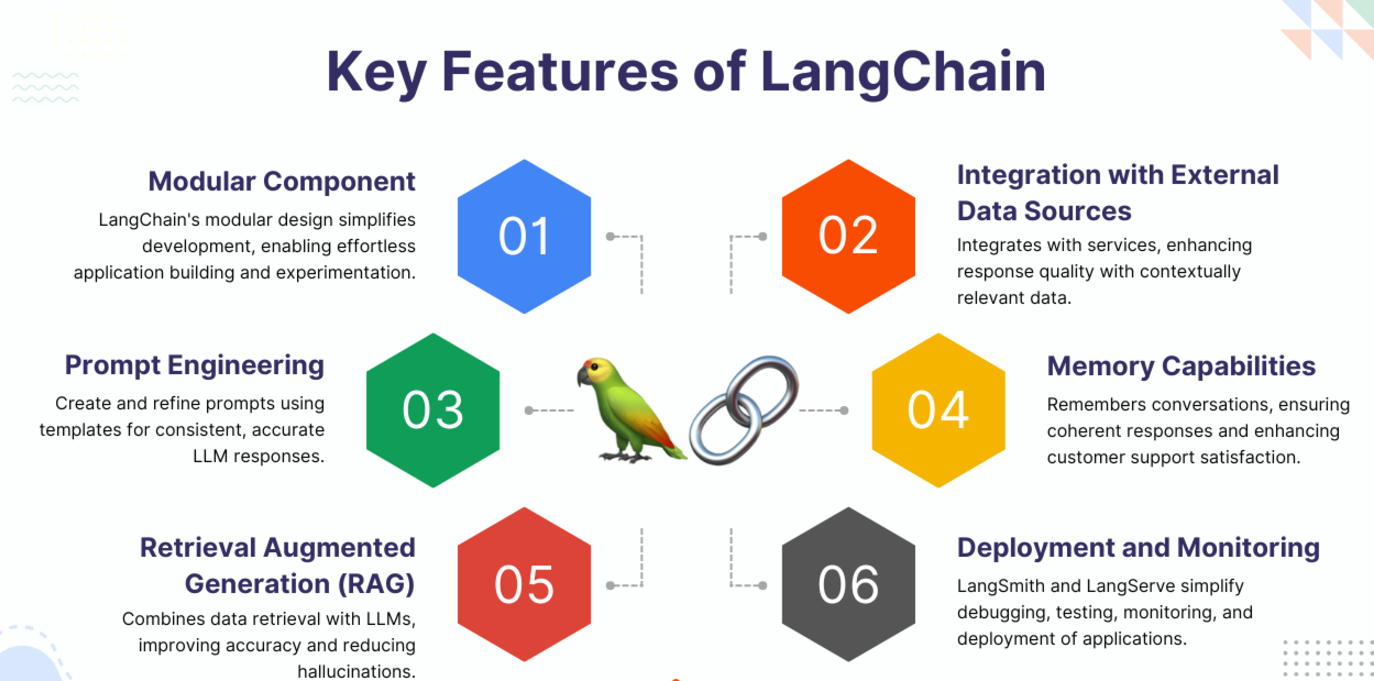
\includegraphics[scale=0.2]{tecnologie/langchain.png}
    \caption{Pricipali funzionalità di \textit{LangChain}}
\end{figure}
\subsubsection{Puppeteer}

\textit{Puppeteer} è una libreria \textit{Node.js} che controlla un \textit{browser Chromium} in modalita \textit{headless} per generare PDF da pagine \textit{web}.
È utile per creare documenti partendo da dei \textit{template}, mantenendo stili e \textit{layout}, e permettendo di personalizzare aspetti come margini e dimensioni della pagina.

\subsubsection{HandleBars}

\textit{Handlebars} è una libreria \textit{JavaScript} per creare e popolare template \textit{HTML} con dati dinamici. 
Consente di separare la logica di presentazione dai dati, supportando espressioni condizionali, \textit{loop} e \textit{helper} personalizzati.

\subsubsection{Servizi \gls{aws}}

\begin{itemize}
\item \textbf{AWS Amplify:} Una piattaforma completa per sviluppare applicazioni \textit{web} e \textit{mobile} con servizi \textit{cloud}. 
Fornisce strumenti per autenticazione, \gls{api}, storage e hosting, semplificando l'integrazione con servizi \gls{aws};
\item \textbf{AWS Cognito:} Un servizio di gestione delle identità che consente agli sviluppatori di aggiungere facilmente funzionalità di autenticazione, registrazione e accesso federato alle proprie applicazioni,
utilizzato inoltre per la generazione di \gls{jwt};
\item \textbf{AWS Bedrock:} Un servizio di intelligenza artificiale generativa offerto da \gls{aws} che consente agli sviluppatori di integrare modelli avanzati di \gls{ai} generativa nelle proprie applicazioni, senza necessità di competenze specifiche in \gls{machine-learning}. 
\textit{AWS Bedrock} supporta modelli pre-addestrati da fornitori \textit{leader} e offre funzionalità per creare, personalizzare e implementare soluzioni \gls{ai} scalabili, ideali per \textit{chatbot}, creazione di contenuti, analisi dei dati e altro;
\item \textbf{AWS S3 (Simple Storage Service):} Un servizio di archiviazione \textit{cloud} offerto da \gls{aws} progettato per il salvataggio di oggetti con scalabilità, disponibilità e sicurezza elevate.
Supporta la memorizzazione e il recupero di qualsiasi quantità di dati, con funzionalità avanzate come versionamento, controllo degli accessi e integrazione con altri servizi \gls{aws}. \\
Nel progetto specifico, \textit{AWS S3} viene utilizzato per archiviare file PDF generati dinamicamente, garantendo un accesso rapido e affidabile.
\end{itemize}

\pagebreak
\subsection{Tecnologie di supporto allo sviluppo}
\label{sez:tecnologie-supporto-sviluppo}

\subsubsection{\gls{npm}}

È il gestore ufficiale dei pacchetti per \textit{Node.js}, utilizzato per installare, condividere e gestire librerie e moduli \textit{JavaScript}. 
Facilita la configurazione e la gestione delle dipendenze nei progetti, rendendo lo sviluppo più efficiente.

\subsubsection{Docker}

Piattaforma che consente di creare e gestire applicazioni in \gls{container} leggeri e portatili.
I \gls{container} permettono l’isolazione delle applicazioni e delle loro dipendenze, garantendo consistenza tra ambienti di sviluppo, \textit{test} e produzione.

\subsubsection{Postman}

Strumento che permette di testare in modo semplice le \gls{api}. 
Consente di inviare richieste \gls{http} ed analizzare le risposte andando a semplificare lo sviluppo ed il \textit{debugging} delle \gls{api}.

\begin{figure}[H]
    \label{fig:postman}
    \centering
    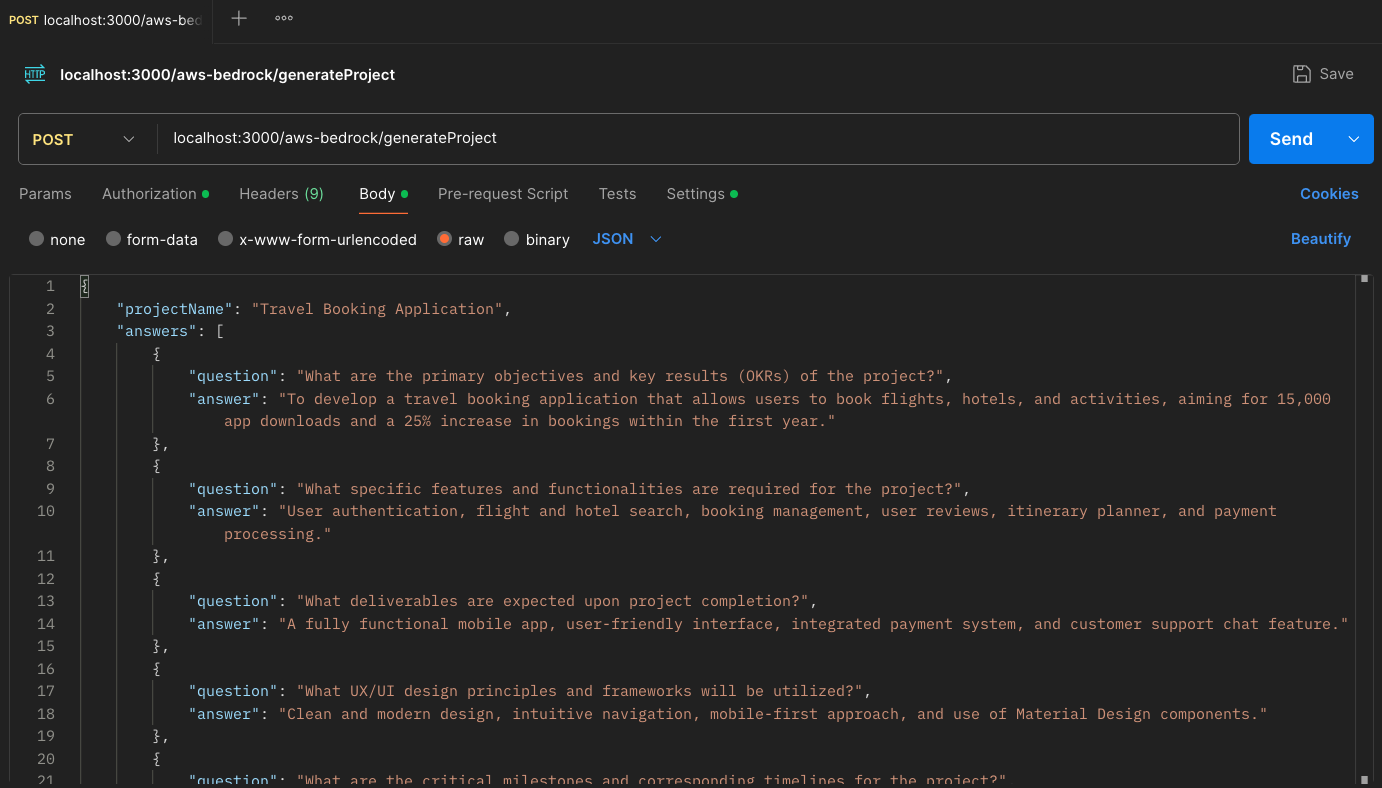
\includegraphics[scale=0.2]{tecnologie/postman.png}
    \caption{Esempio di utilizzo di \textit{Postman} per chiamata \gls{api}}
\end{figure}

\subsubsection{StarUML}

Uno strumento avanzato per la modellazione di \gls{uml}, utilizzato per creare e gestire diagrammi di progettazione software. Supporta un'ampia gamma di diagrammi \gls{uml}, tra cui casi d'uso, sequenza e attività, semplificando la visualizzazione di architetture e flussi.
È stato utilizzato per creare i diagrammi dei casi d’uso del progetto.

\subsubsection{git}

Un sistema di controllo di versione distribuito, progettato per tracciare le modifiche al codice sorgente e facilitare la collaborazione tra sviluppatori. \\
Permette di gestire versioni, ramificare progetti e integrare modifiche in modo efficiente e sicuro. 

\pagebreak
\subsubsection{MongoDB Compass}

Un'interfaccia grafica intuitiva per interagire con \textit{database MongoDB}, che consente di esplorare e modificare i dati, visualizzare indici e \textit{query},
e semplificare la gestione e l'analisi del \textit{database.}

\begin{figure}[H]
    \label{fig:mongodb-compass}
    \centering
    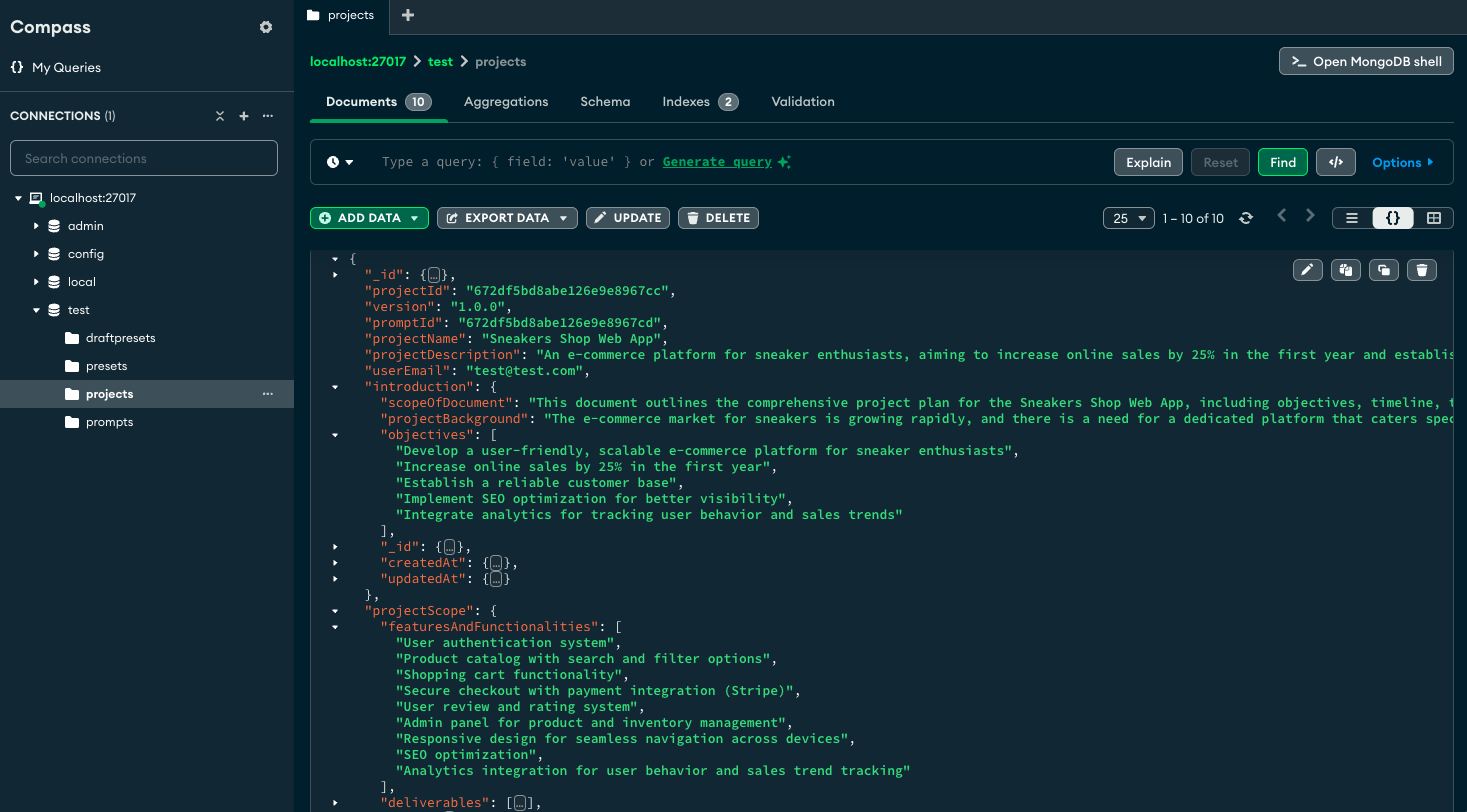
\includegraphics[scale=0.2]{tecnologie/mongodb-compass.png}
    \caption{Visualizzazione di un documento in \textit{MongoDB Compass}}
\end{figure}

\subsection{Tecnologie di verifica e validazione del codice}
\label{sez:tecnologie-validazione-codice}

\subsubsection{Jest}

\textit{Jest} è un \textit{framework} di \textit{testing JavaScript} progettato per garantire la qualità del codice, supportando \textit{test} unitari, di integrazione e \textit{snapshot}.
Grazie alla sua semplicità, velocità e funzionalità avanzate, è ideale per \textit{test} automatizzati nei progetti moderni.

\subsubsection{React Testing Library}

Una libreria per testare componenti \textit{React}, che si concentra sull'interazione dell'utente piuttosto che sull'implementazione interna. 
Fornisce strumenti per simulare eventi e verificare il comportamento dell'interfaccia utente in modo semplice e affidabile.

\subsubsection{Prettier}

Uno strumento di formattazione automatica del codice che garantisce uno stile uniforme, migliorando la leggibilità e la manutenzione del codice. 
Supporta diversi linguaggi e può essere integrato facilmente nei flussi di lavoro di sviluppo.

\pagebreak
\subsubsection{ESLint}

Uno strumento di \textit{linting} per \textit{JavaScript} che aiuta a individuare e correggere errori nel codice, andando a migliorarne qualità e coerenza.
Supporta configurazioni personalizzabili e integrazioni con \gls{ide} per un'esperienza di sviluppo più fluida.

\begin{figure}[H]
    \label{fig:eslint}
    \centering
    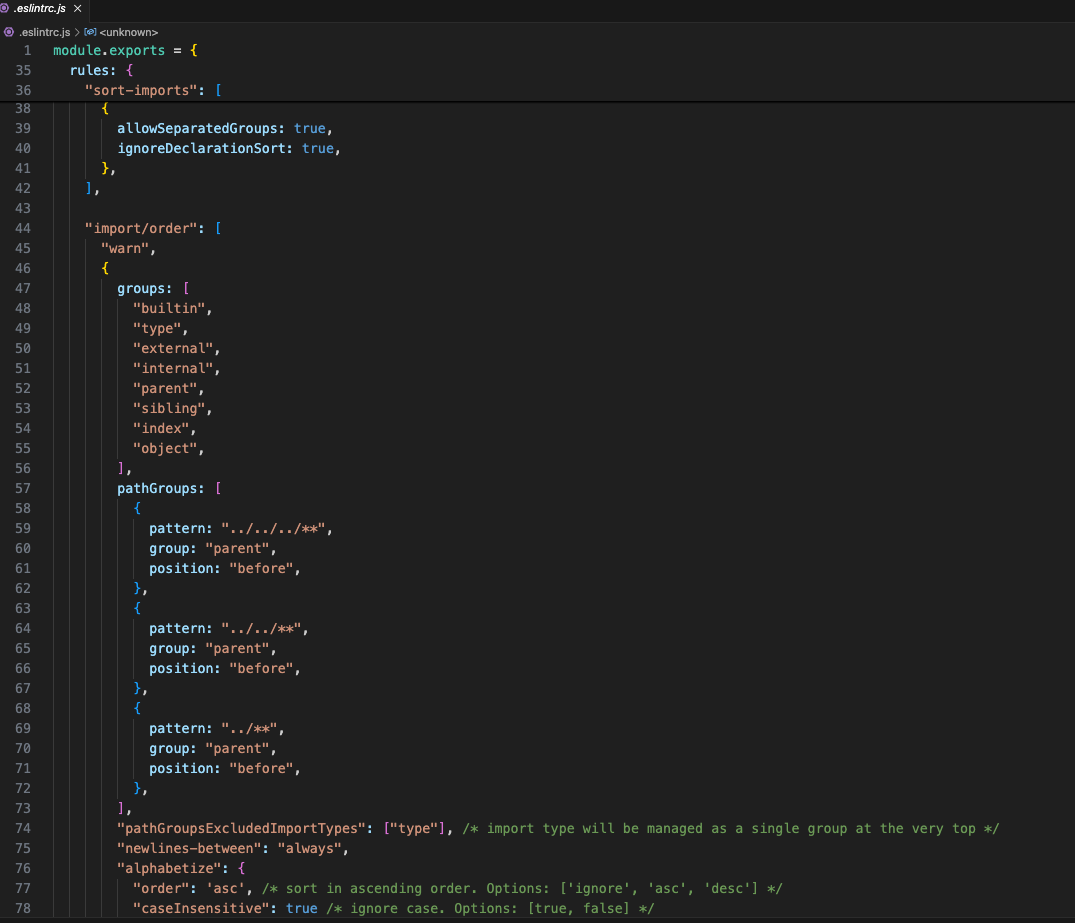
\includegraphics[scale=0.2]{tecnologie/eslint.png}
    \caption{Esempio di configurazione di \textit{ESLint}}
\end{figure}

\pagebreak
\section{Propensione aziendale all'innovazione}
\label{sez:propensione-a-innovazione}

L'azienda Zero12 è profondamente orientata all'innovazione e alla sperimentazione di nuove tecnologie.\\
In qualità di partner di \gls{aws}, la società si distingue per l'interesse nella ricerca e nello sviluppo nel campo dei servizi \textit{cloud}.\\ 

\noindent Durante il mio periodo di \textit{stage}, diversi membri dell'azienda hanno partecipato a conferenze in Emilia Romagna, organizzate presso la sede di UAN Company, acquisitrice di Zero12, per esplorare nuove tecnologie e come queste possano essere integrate nei progetti futuri dell'azienda.\\ 
Mi è stato riferito che tali conferenze e corsi di formazione sono eventi frequenti, in quanto Zero12 promuove attivamente la formazione continua per tutti i suoi dipendenti, riflettendo il suo impegno per il miglioramento e l'evoluzione costante delle competenze interne.
    \chapter{Progetto di stage}
\label{cap:introduzione-al-progetto}

\section{Gestione aziendale degli \textit{stage}}  
\label{sez:gestione-aziendale-stage}  

\textbf{Zero12} considera gli \textit{stage} con gli studenti dell'Università di Padova un'opportunità molto importante per formare nuove risorse umane,
per far conoscere l'azienda e per valutare possibili nuove tecnologie.\\  
Grazie all'evento \textit{STAGE-IT}, svolto ad aprile 2024 e promosso da Confindustria Veneto Est e dall'Università di Padova, 
l'azienda ha avuto l'opportunità di presentarsi agli studenti e di esporre i propri progetti di \textit{stage}.\\  

\noindent Gli \textit{stage} permettono agli studenti di applicare le conoscenze acquisite durante il corso di studi, 
di confrontarsi con un ambiente lavorativo reale e di sviluppare competenze professionali.\\  
Per l'azienda, questi progetti rappresentano un ottimo strumento per sperimentare nuove idee da presentare a potenziali clienti, 
oltre che per formare future risorse umane.\\  
Questo è dimostrato dal fatto che molti attuali dipendenti sono stati assunti dopo aver svolto uno \textit{stage} presso l'azienda.\\  
Tutti i colleghi sono molto disponibili e pronti ad aiutare, al fine di rendere la permanenza dello stagista il più produttiva e piacevole possibile.\\  

\section{Descrizione proposta di \textit{stage}}
\label{sez:descrizione-stage}

L'idea alla base dello \textit{stage} è quella di automatizzare la creazione di un documento denominato \texttt{Allegato Tecnico}.\\  
Questo documento raccoglie tutte le informazioni tecniche relative ad un progetto \textit{software}, comprese le tecnologie utilizzate,
la struttura del progetto, le scelte architetturali ed il piano di \textit{testing}, per citare alcune delle sezioni.\\  
Fino ad oggi, l'azienda ha sempre realizzato questo documento manualmente.\\
Tuttavia, con l'aumento dei progetti e delle risorse impiegate,
l'introduzione di un \textit{tool} per automatizzare questo processo, anche solo parzialmente, risulta particolarmente interessante.\\  

\pagebreak
\noindent L'obiettivo dello \textit{stage} è quindi la realizzazione di una piattaforma \textit{web} che, tramite l'uso di sistemi di \gls{generative-ai},  
permetta di generare automaticamente questo documento.\\  
L'utente finale della piattaforma sarà un membro del \textit{team} di sviluppo od il \textit{project-manager}.\\  
Questi andrà a compilare dei \textit{Preset}, ovvero una serie di domande create \textit{ad hoc}
per raccogliere le informazioni necessarie alla creazione del documento, ottimizzate in base al tipo di progetto da sviluppare (ad esempio, una \textit{Web App} o una \textit{Mobile App}).\\  
Il sistema utilizzerà i servizi di \gls{generative-ai} forniti da \gls{aws} per creare il documento automaticamente.\\  

\noindent Una volta generato, l'utente avrà la possibilità di rigenerare il documento, in parte o nella sua totalità, inserendo un \gls{prompt}.\\  
Questo \gls{prompt} sarà una frase o un paragrafo che guiderà il sistema, consentendo all'utente di specificare le migliorie o modifiche da apportare al documento.\\  
Tutte le versioni del documento verranno salvate, permettendo di visualizzare le differenze tra una versione e l'altra.\\  
Una volta soddisfatto del risultato, l'utente potrà scaricare il documento in formato \textit{PDF}.\\  
La {\hyperref[fig:project-schema]{Figura 2.1}} mostra uno schema che rappresenta l'idea alla base del progetto.\\  


\begin{figure}[H]
    \label{fig:project-schema}
    \centering
    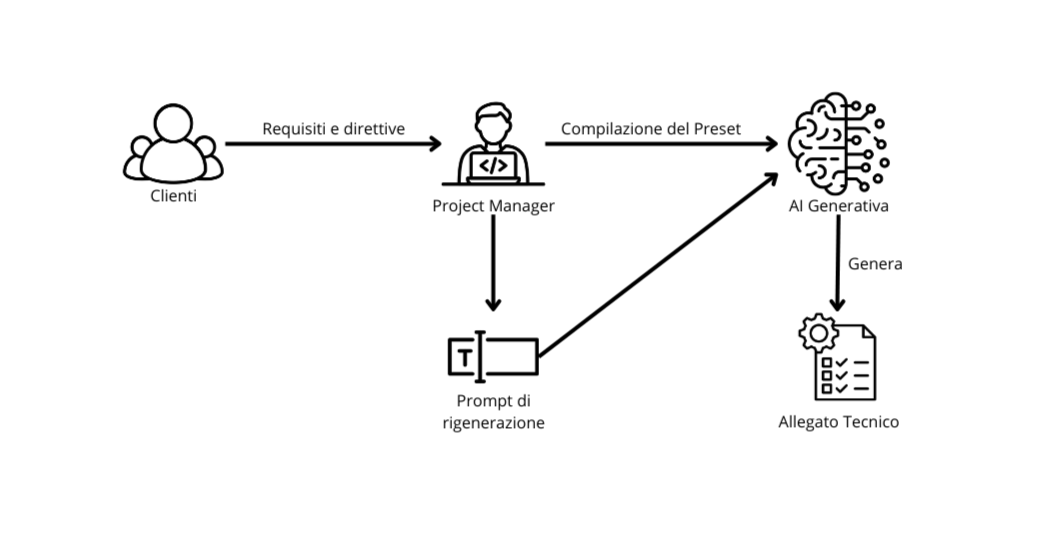
\includegraphics[scale=0.6]{gen-ai-documentation-schema.png}
    \caption{Schema del progetto}
\end{figure}
\section{\textit{Large Language Models}}
\label{sez:llm}

\subsection{Introduzione}
\label{subsec:llm-introduzione}

Descrizione di cos'è un Large Language Model (LLM), per cosa vengono usati, come si applica all'interno del progetto, ecc.

\subsection{Confronto tra principali LLM}
\label{subsec:llm-confronto}

Confronto tra i principali Large Language Models, come GPT-4, Anthropic Claude 3.5 Sonnet, ecc., per capire le differenze tra di loro, per cosa vengono usati, ecc.
\subsection{Confronto tra principali LLM}
\label{subsec:llm-confronto}

Di seguito è presente un confronto tra i principali \gls{llm} attualmente disponibili sul mercato\footcite{site:key-differences-llm}, con l'obiettivo di evidenziare le loro differenze, i casi d'uso principali, i loro punti di forza ed i limiti di ciascun modello.\\
Questi modelli sono accessibili tramite \textit{AWS Bedrock}\footcite{site:aws-bedrock}, ad eccezione di \textit{GPT-4}, incluso comunque nel confronto per la sua rilevanza e diffusione.

\subsubsection{\textit{GPT-4 (OpenAI)}}

\noindent \textbf{Descrizione:}
\textit{GPT-4} è un modello all’avanguardia progettato per risolvere compiti complessi grazie alla sua elevata capacità di comprensione e generazione del linguaggio. \\
Anche se non disponibile tramite \textit{AWS Bedrock}, è una delle soluzioni più utilizzate per la sua accuratezza e versatilità.\\

\noindent \textbf{Casi d’uso:}
\begin{itemize}
   \item \textbf{Generazione tecnica:} Creazione di documentazione tecnica dettagliata;
   \item \textbf{Analisi avanzata:} Interpretazione di dati e contenuti complessi;
   \item \textbf{Supporto per sviluppatori:} \textit{Debugging} e generazione di codice ottimizzato;
   \item \textbf{Ricerca scientifica:} Sintesi e analisi di \textit{paper} scientifici.
\end{itemize}

\noindent \textbf{Punti di forza:}
\begin{itemize}
    \item \textbf{Capacità di contesto estesa:} Supporta fino a 32k \gls{token}, adatto per documenti complessi;
    \item \textbf{Versatilità \textit{multi-task}:} Funziona bene su domande aperte e contesti tecnici specifici;
    \item \textbf{\textit{Fine-tuning} implicito:} Non necessita di \textit{tuning} per molti casi d’uso, grazie ad un addestramento generale molto efficace.
\end{itemize}

\noindent \textbf{Limiti:}
\begin{itemize}
    \item \textbf{Costo elevato:} Il prezzo per \gls{token} è più alto rispetto ad altre opzioni;
    \item \textbf{Latenza:} \textit{Input} complessi possono rallentare il tempo di risposta.
    \item \textbf{Non nativo per \textit{AWS Bedrock}:} Necessita di integrazione tramite \gls{api} \textit{OpenAI}.
\end{itemize}

\vspace{1.5cm}
\subsubsection{\textit{Claude 3.5 Sonnet (Anthropic)}}

\noindent \textbf{Descrizione:}
\textit{Claude 3.5 Sonnet} è ottimizzato per la gestione di contesti estesi e la generazione di risposte sicure e trasparenti. \\\
Su \textit{AWS Bedrock}, è utilizzato per applicazioni con grandi volumi di testo e analisi linguistiche. \\

\noindent \textbf{Casi d’uso:}
\begin{itemize}
    \item \textbf{Analisi documentale:} Generazione e sintesi di documenti di grandi dimensioni (fino a 100k \gls{token});
    \item \textbf{Automazione \textit{HR} e legale:} Risposte standardizzate e conformità normativa;
    \item \textbf{Interfacce conversazionali:} \textit{Chatbot} sicuri per il supporto clienti ed interno.
\end{itemize}

\noindent \textbf{Punti di forza:}
\begin{itemize}
    \item \textbf{Capacità di contesto estesa:} Supporta \textit{input} fino a 100k \gls{token}, ideale per documenti lunghi;
    \item \textbf{Bias ridotto:} Allenato per minimizzare risposte non sicure o inappropriate;
    \item \textbf{Costi contenuti:} Efficiente rapporto costo\textit{-token}.
\end{itemize}

\noindent \textbf{Limiti:}
\begin{itemize}
    \item \textbf{Latenza:} \textit{Input} complessi possono rallentare il tempo di risposta;
    \item \textbf{Risposte conservative:} Tende a evitare \textit{output} creativi o fuori dall’ordinario.
    \item \textbf{Limitato per codice:} Meno supporto per generazione di codice avanzato.
\end{itemize}

\subsubsection{\textit{Amazon Titan}}

\noindent \textbf{Descrizione:}
\textit{Titan} è il modello di intelligenza artificiale sviluppato da \textit{Amazon}, ottimizzato per l’integrazione nativa con \textit{AWS Bedrock} ed altre soluzioni \gls{aws}.\\
Si concentra su casi d’uso aziendali pratici e robusti.\\

\noindent \textbf{Casi d’uso:}
\begin{itemize}
    \item \textbf{Elaborazione dati strutturati:} Supporto per analisi di \textit{report} aziendali e \textit{database};
    \item \textbf{\textit{Chatbot} aziendali:} Personalizzabili per specifici settori industriali;
    \item \textbf{Supporto operativo:} Automazione di flussi di lavoro e riepiloghi aziendali.
\end{itemize}

\noindent \textbf{Punti di forza:}
\begin{itemize}
    \item \textbf{Integrazione nativa con \gls{aws}:} Compatibilità totale con strumenti \gls{aws} come \textit{DynamoDB} e \textit{S3};
    \item \textbf{Ottimizzazione della sicurezza:} Protezione dei dati aziendali con politiche \gls{aws} rigorose;
    \item \textbf{Efficienza nei costi:} Disegnato per fornire prestazioni elevate anche con \textit{budget} contenuti.
\end{itemize}

\noindent \textbf{Limiti:}
\begin{itemize}
    \item \textbf{Capacità di linguaggio generico inferiore:} Non raggiunge la qualità linguistica di \textit{GPT-4} o \textit{Claude 3.5};
    \item \textbf{Meno innovativo:} Adatto a compiti definiti, non eccelle in creatività o flessibilità;
    \item \textbf{Limitata flessibilità:} Richiede configurazioni specifiche per settori diversi.
\end{itemize}

\vspace{1.5cm}
\subsubsection{\textit{Llama (Meta)}}

\noindent \textbf{Descrizione:}
\textit{Llama} è un modello \textit{open-source} progettato per essere altamente personalizzabile, ideale per casi in cui è richiesto un controllo completo sul \textit{fine-tuning}. 
Su \textit{AWS Bedrock}, è particolarmente utile per applicazioni che richiedono soluzioni specifiche per il dominio applicativo.\\

\noindent \textbf{Casi d’uso:}
\begin{itemize}
    \item \textbf{Addestramento personalizzato:} Modelli ottimizzati per domini ristretti come finanza o medicina;
    \item \textbf{Soluzioni locali:} Applicazioni in ambienti chiusi per garantire massima \textit{privacy};
    \item \textbf{Sperimentazione:} Perfetto per ricerca accademica e/o sviluppo di prototipi.
\end{itemize}

\noindent \textbf{Punti di forza:}
\begin{itemize}
    \item \textbf{\textit{Open-source}:} Offre pieno controllo per modifiche e ottimizzazioni;
    \item \textbf{Scalabilità flessibile:} Può essere ridimensionato per applicazioni \textit{on-premises} o \textit{cloud}.
\end{itemize}

\noindent \textbf{Limiti:}
\begin{itemize}
    \item \textbf{Richiede competenze tecniche avanzate:} Il \textit{tuning} e l’implementazione necessitano di risorse specializzate;
    \item \textbf{Prestazioni inferiori senza \textit{tuning}:} Il modello base è meno performante rispetto a \textit{GPT-4} o \textit{Claude 3.5};
    \item \textbf{Ambiente di sviluppo più complesso:} Meno pronto all’uso rispetto ai modelli pre-addestrati.
\end{itemize}

\noindent Di seguito una tabella che mostra un confronto riassuntivo tra i modelli presentati:

\begin{table}[H]
    \centering
    \rowcolors{2}{gray!15}{white} % Righe alternate: grigio chiaro e bianco
    \begin{tabularx}{\textwidth}{|>{\centering\arraybackslash}X|>{\centering\arraybackslash}X|>{\centering\arraybackslash}X|>{\centering\arraybackslash}X|}
        \hline
        \rowcolor{green!30} % Colore dell'intestazione: verde chiaro
        \textbf{Modello} & \textbf{Casi d'uso} & \textbf{Punti di forza} & \textbf{Limiti} \\
        \hline
        \textit{GPT-4} & Automazione avanzata, analisi tecnica & Supporta 32k \textit{token}, versatile e accurato & Costoso, non nativo su \textit{AWS Bedrock} \\
        \hline
        \textit{Claude 3.5} & Generazione documenti lunghi, chatbot sicuri & Contesto ampio, sicurezza nei dati & Risposte conservative, latenza elevata \\
        \hline
        \textit{Amazon Titan} & Report aziendali, automazione & Integrazione nativa \gls{aws}, costi ridotti & Meno versatile, output linguistico generico \\
        \hline
        \textit{Llama} & Addestramento personalizzato & \textit{Open-source}, flessibilità & Prestazioni limitate senza modifiche avanzate \\
        \hline
    \end{tabularx}
    \caption{Tabella confronto riassuntivo \textit{LLM}}
    \label{tab:confronto-lllm}
\end{table}

\pagebreak
\section{Obiettivi aziendali}
\label{sez:obiettivi-aziendali}

Gli obiettivi forniti dall'azienda sono stati definiti a priori dell'inizio dello stage all'interno del documento del Piano di Lavoro, essi si suddividono in:
\begin{itemize}
    \item \textbf{OO: Obiettivi obbligatori}, sono gli obiettivi minimi che devono essere raggiunti per considerare lo stage completato con successo;
    \item \textbf{OD: Obiettivi desiderabili}, sono gli obiettivi non necessari, ma che vanno ad aggiungere valore al prodotto finito;
    \item \textbf{OF: Obiettivi facoltativi}, sono gli obiettivi opzionali, non necessari per il completamento del progetto.
\end{itemize}

\noindent All'interno della seguente tabella sono elencati gli obiettivi aziendali dello stage, aventi la seguente nomeclatura:

\begin{center}
    \textbf{R}-\textbf{N}
\end{center}

Dove:
\begin{itemize}
    \item $\textbf{R} \in  \{OO, OD, OF\}$ rappresentante la tipologia di obiettivo; \\
    \item $\textbf{N} \in N$ rappresentante il numero progressivo dell'obiettivo.
\end{itemize}


\renewcommand{\arraystretch}{1.5} % Increases the row height for better vertical space

\begin{longtable}{|c|>{\centering\arraybackslash}p{0.7\textwidth}|} % Adjust the column width with p{0.7\textwidth}
    \hline
    \rowcolor{green!30} % Header color: light green
    \textbf{Codice Obiettivo} & \textbf{Descrizione Obiettivo} \\
    \hline
    \endfirsthead % Start of the table, first header
    
    \hline
    \rowcolor{green!30} % Header color on subsequent pages
    \textbf{Codice Obiettivo} & \textbf{Descrizione Obiettivo} \\
    \hline
    \endhead % Continuation of the table (repeats on every page)
    
    \hline
    \multicolumn{2}{|c|}{\rowcolor{green!30} \textbf{Obiettivi Obbligatori}} \\
    \hline % Adds a horizontal line after the header row
    \textbf{OO-1} & \textbf{Apprendimento delle tecnologie di sviluppo:} Acquisire competenze pratiche nell'uso di \textit{React}, \textit{NestJS} e \textit{MongoDB} per la progettazione e lo sviluppo di applicazioni. \\

    \hline
    \textbf{OO-2} & \textbf{Gestione del versionamento del codice:} Apprendere l'uso di \textit{Git} e adottare \textit{Git Flow} come metodologia per il controllo delle versioni e la collaborazione. \\
    \hline
    \textbf{OO-3} & \textbf{Analisi e scelta del \gls{llm}:} Valutare i modelli disponibili per selezionare quello più adatto al progetto. \\
    \hline
    \textbf{OO-4} & \textbf{Introduzione alle metodologie agili:} Familiarizzare con le metodologie agili di sviluppo per la gestione efficace di progetti. \\
    \hline
    \textbf{OO-5} & \textbf{Pianificazione e gestione giornaliera:} Imparare a gestire \textit{task} e obiettivi giornalieri allineati al piano di lavoro. \\
    \hline
    \textbf{OO-6} & \textbf{Sviluppo di una \textit{web app:}} Progettare e realizzare un'applicazione \textit{web} per consentire l'interazione dell'utente con la piattaforma. \\
    \hline
    \textbf{OO-7} & \textbf{Sviluppo e integrazione con \gls{ai-generativa}:} Implementare i flussi logici del progetto e integrare i servizi di \gls{ai-generativa} scelti. \\
    \hline
    \textbf{OO-8} & \textbf{Documentazione \gls{api}:} Creare una documentazione \textit{Swagger} per le \gls{api} sviluppate. \\
    \hline
    \textbf{OO-9} & \textbf{Documento di analisi progettuale:} Redigere un documento tecnico che descriva l'architettura e le componenti principali della piattaforma. \\
    \hline
    \textbf{OO-10} & \textbf{\textit{User Story Mapping:}} Realizzare una mappatura delle \gls{user-stories} per descrivere e organizzare i requisiti del progetto. \\
    \hline
    \multicolumn{2}{|c|}{\rowcolor{green!30} \textbf{Obiettivi Desiderabili}} \\
    \hline % Adds a horizontal line after the subtitle
    \textbf{OD-1} & \textbf{Comparazione tra modelli \gls{llm}:} Effettuare un'analisi comparativa tra almeno due \gls{llm} per verificarne le differenze in termini di prestazioni, funzionalità e costi. \\
    \hline
    \multicolumn{2}{|c|}{\rowcolor{green!30} \textbf{Obiettivi Facoltativi}} \\
    \noalign{\hrule} % Adds a horizontal line after the subtitle
    \textbf{OF-1} & \textbf{Piattaforma di amministrazione:} Creare una piattaforma \textit{admin} per la gestione dei \textit{Preset} e dei modelli \gls{llm}. \\
    \hline
    \caption{Obiettivi aziendali dello \textit{stage}} % Table caption
    \label{tab:obiettivi_stage} % Label for referencing the table
\end{longtable}

\section{Vincoli}
\label{sez:vincoli}

\subsection{Vincoli tecnologici}
\label{subsec:vincoli-tecnologici}

Utilizzo di ReactJs come framework frontend, NestJs come backend, MongoDB come database, creazione di API Restful, ecc.

\subsection{Vincoli organizzativi}
\label{subsec:vincoli-organizzativi}

Utilizzo di Jira per la gestione del lavoro, Slack per la comunicazione interna, comunicazione costante con il tutor aziendale, comunicazione settimanale con il relatore, ecc.

\subsection{Prodotti attesi}
\label{subsec:prodotti-attesi}

Descrizione di quali prodotti sono attesi, come web app, API, documentazione, ecc.\\
\section{Obiettivi personali}
\label{sez:obiettivi-personali}

La scelta di intraprendere questo progetto di \textit{stage} è stata motivata da diversi fattori che ritengo molto rilevanti per la mia crescita professionale e per il mio interesse verso tematiche innovative e tecnologiche.\\

\noindent Di seguito sono elencate le motivazioni principali:

\begin{itemize}
    \item \textbf{Tema del progetto:} L'\gls{generative-ai} è un campo estremamente affascinante e in continua evoluzione, con applicazioni che spaziano in molti settori.\\
    L'opportunità di lavorare su un progetto che utilizza queste tecnologie rappresenta una sfida stimolante ed un'occasione unica per approfondire le mie conoscenze in un contesto pratico;
    \item \textbf{Prima impressione a \textit{StageIT}:} Il colloquio tenuto con i rappresentanti aziendali a \textit{StageIT}, un evento tenuto ad Aprile 2024 che permette alle aziende di presentare i propri progetti di \textit{stage}, è risultato molto interessante. \\
    L'incontro con alcuni dei dipendenti aziendali mi ha fatto una buonissima impressione, si sono dimostrati molto disponibili nel rispondere alle mie domande ed ho trovato stimolante il loro entusiasmo nell'affrontare tematiche tecnologiche avanzate;
    \item \textbf{Utilizzo di servizi \gls{aws}:} Sono molto interessato ai servizi \gls{aws}, che considero fondamentali nel contesto lavorativo odierno. \\
    \gls{aws} offre una vasta gamma di servizi \textit{cloud}, essenziali per lo sviluppo di applicazioni moderne e scalabili, e credo che acquisire esperienza con questi strumenti possa essere un vantaggio significativo per la mia carriera lavorativa.\\
    Essendo Zero12 un partner \gls{aws}, questo progetto mi offre l'opportunità di lavorare con questi servizi in un contesto pratico e reale;
    \item \textbf{Tecnologie all'avanguardia:} Rispetto ad altre aziende con cui ho avuto colloqui, questa si distingue per l'adozione di tecnologie moderne e innovative. \\
    L'opportunità di lavorare con tecnologie all'avanguardia rappresenta una grande opportunità di apprendimento;
    \item \textbf{Posizione geografica:} L'azienda si trova a circa 40 minuti dalla mia residenza, in una posizione comoda e ben collegata, che rende semplice e pratico il tragitto quotidiano;
    \pagebreak
    \item \textbf{\textit{Team} giovane e dinamico:} Dopo aver parlato con alcuni studenti che avevano già svolto lo \textit{stage} in azienda, mi è stato riferito che l'ambiente di lavoro è molto positivo.\\
    Il \textit{team} giovane e dinamico è altamente collaborativo e orientato alla crescita professionale, creando un contesto ideale per lo sviluppo delle competenze.
\end{itemize}


\noindent Gli obiettivi personali rappresentano le competenze e le conoscenze che mi sono imposto di acquisire durante il mio periodo di \textit{stage}.\\

\noindent Questi obiettivi sono legati al miglioramento e allo sviluppo delle proprie capacità professionali, sia dal punto di vista tecnico che umano.
La loro definizione aiuta a focalizzarsi su aree specifiche di crescita e a pianificare il percorso formativo in modo mirato. \\

\noindent Nel contesto del mio stage, gli obiettivi personali possono essere suddivisi in tre categorie principali:

\begin{itemize}
    \item \textbf{Obiettivi tecnici}: Si concentrano sull'acquisizione di nuove competenze tecniche, come l'apprendimento di linguaggi di programmazione, l'utilizzo di \textit{framework}, e l'esplorazione di tecnologie avanzate.
    \item \textbf{Obiettivi di crescita personale}: Riguardano lo sviluppo delle \textit{soft skills}, come la gestione del tempo, la comunicazione professionale e la comprensione del contesto aziendale.
    \item \textbf{Obiettivi di autonomia e collaborazione}: Focalizzati sul miglioramento della capacità di lavorare autonomamente e di collaborare efficacemente con i colleghi.
\end{itemize}

\noindent All'interno della seguente tabella sono riportati gli obiettivi personali, aventi la seguente nomenclatura:

\begin{center}
    \textbf{OP}-\textbf{N}
\end{center}

Dove:
\begin{itemize}
    \item OP sta per Obiettivo Personale; \\
    \item $\textbf{N} \in N$ rappresentante il numero progressivo dell'obiettivo.
\end{itemize}

\renewcommand{\arraystretch}{1.5} % Increases the row height for better vertical space

\begin{longtable}{|c|>{\centering\arraybackslash}p{0.7\textwidth}|} % Adjust the column width with p{0.7\textwidth}
    \hline
    \rowcolor{green!30} % Header color: light green
    \textbf{Codice Obiettivo} & \textbf{Descrizione Obiettivo} \\
    \hline
    \endfirsthead % Start of the table, first header
    
    \hline
    \rowcolor{green!30} % Header color on subsequent pages
    \textbf{Codice Obiettivo} & \textbf{Descrizione Obiettivo} \\
    \hline
    \endhead % Continuation of the table (repeats on every page)
    
    \hline
    \multicolumn{2}{|c|}{\rowcolor{green!30} \textbf{Obiettivi Personali}} \\
    \hline
    \textbf{OP-1} & \textbf{Padroneggiare nuovi linguaggi e \textit{framework}:} Acquisire competenze avanzate nello sviluppo di applicazioni utilizzando \textit{React} per il \gls{frontend} e \textit{NestJS} per il \gls{backend}, implementando progetti reali che sfruttano queste tecnologie. \\
    \hline
    \textbf{OP-2} & \textbf{Esplorare i servizi \textit{cloud} di \gls{aws}:} Imparare ad utilizzare servizi come \textit{AWS Amplify}, \textit{AWS Cognito}, \textit{AWS S3}, e \textit{AWS Bedrock}, comprendendo come integrarli in un’architettura scalabile e moderna. \\
    \hline
    \textbf{OP-3} & \textbf{Competenze in \gls{generative-ai}:} Sviluppare un solido \textit{know-how} nell’utilizzo di tecnologie di \gls{generative-ai}, come l’integrazione di modelli \textit{AI (Claude, GPT)} in progetti pratici. \\
    \hline
    \multicolumn{2}{|c|}{\rowcolor{green!30} \textbf{Obiettivi di Crescita Personale}} \\
    \hline
    \textbf{OP-4} & \textbf{Comprendere il settore professionale:} Ottenere una visione del contesto aziendale del settore tecnologico, analizzando flussi di lavoro e \textit{trend} di mercato, per orientare al meglio il percorso professionale futuro. \\
    \hline
    \textbf{OP-5} & \textbf{Ottimizzare la gestione del tempo:} Sviluppare un approccio strutturato al lavoro, utilizzando strumenti di produttività e tecniche di prioritizzazione per rispettare scadenze e migliorare l’efficienza personale. \\
    \hline
    \textbf{OP-6} & \textbf{Comunicazione professionale efficace:} Rafforzare le capacità di comunicazione scritta e orale per facilitare il dialogo e le collaborazioni. \\
    \hline
    \multicolumn{2}{|c|}{\rowcolor{green!30} \textbf{Obiettivi di Autonomia e Collaborazione}} \\
    \hline
    \textbf{OP-7} & \textbf{Lavoro indipendente:} Incrementare la capacità di gestire \textit{task} e progetti in modo autonomo, prendendo decisioni informate e risolvendo problemi complessi senza supervisione diretta. \\
    \hline
    \textbf{OP-8} & \textbf{Collaborazione proattiva:} Contribuire attivamente al lavoro di squadra, partecipando a \textit{meeting}, condividendo idee e accogliendo \textit{feedback} per migliorare continuamente le proprie performance. \\
    \hline
    \caption{Obiettivi personali dello \textit{stage}} % Table caption
    \label{tab:obiettivi-personali-stage} % Label for referencing the table
\end{longtable}


    \chapter{Svolgimento dello \textit{stage}}
\label{cap:svolgimento-dello-stage}

\section{Pianificazione delle attività}
\label{sez:pianificazione-attivita}

La pianificazione delle attività è stata effettuata seguendo un approccio iterativo e collaborativo, con l'obiettivo di garantire una gestione efficace del progetto.\\
Durante la prima settimana, ho lavorato alla definizione delle \gls{user-stories}, che hanno permesso di identificare e organizzare le funzionalità principali del progetto in base alla priorità e al valore per l’utente.\\
Per la lista delle \gls{user-stories} si veda la {\hyperref[subsubsec:epic-stories]{sezione §3.3.1}}.\\

\noindent Successivamente, insieme al \textit{tutor} aziendale, le attività sono state suddivise in \gls{sprint} settimanali.\\
In ogni \gls{sprint} abbiamo selezionato specifiche \gls{user-stories} da completare, tenendo conto delle loro priorità, mantenendo un carico di lavoro sostenibile per il periodo di una settimana. \\
Per ciascun \gls{sprint} sono stati definiti dei criteri di accettazione, ovvero parametri chiari e verificabili che indicano quando un'attività può essere considerata completata. \\
Questi criteri, stabiliti in collaborazione con il \textit{tutor} aziendale, hanno assicurato una qualità elevata del lavoro svolto ed una comprensione condivisa degli obiettivi. \\
Questo approccio ha permesso di monitorare costantemente i progressi e garantire un miglioramento continuo durante ogni iterazione del progetto.


\pagebreak
\subsection{Pianificazione settimanale}
\label{sez:pianificazione-settimanale}

\section*{\textit{Sprint} 1: Studio tecnologie (25 Settembre - 1 Ottobre)}
\textbf{Obiettivo:} Studio delle tecnologie fondamentali per il progetto, creazione \gls{user-stories} e della pianificazione.\\  

\noindent \textbf{Descrizione:}\\  
\noindent In questo \gls{sprint}, l'obiettivo principale è acquisire familiarità con le tecnologie che verranno utilizzate nel progetto, come \textit{AWS Bedrock}, \textit{AWS Cognito}, \textit{React}, \textit{NestJS}, \textit{MongoDB}, \textit{Puppeteer} ed altri strumenti correlati.\\
Ho inoltre stilato le \gls{user-stories} e la pianificazione settimanale.\\

\noindent \textbf{Criteri di accettazione:}  
\begin{itemize}
    \item Sono state create tutte le \gls{user-stories} necessarie per la pianificazione del progetto;
    \item È stata stilata una pianificazione dettagliata, suddivisa in \gls{sprint} settimanali, che definisce le attività principali del progetto;
    \item Lo stagista ha acquisito una conoscenza di base sufficiente delle tecnologie per iniziare le implementazioni nei successivi \gls{sprint}.
\end{itemize}
\section*{\textit{Sprint} 2: Implementazione autenticazione con \textit{AWS Cognito} (2 Ottobre - 8 Ottobre)}
\textbf{Obiettivo:} Implementare il sistema di autenticazione utilizzando \textit{AWS Cognito}.\\  

\noindent \textbf{Descrizione:}\\  
\noindent Questo \gls{sprint} si concentra sull'implementazione del flusso di \textit{login} per gli utenti utilizzando \textit{AWS Cognito}. \\
Ho sviluppato il sistema di autenticazione e autorizzazione, consentendo agli utenti di accedere e gestire il proprio \textit{account}. \\
Ho inoltre implementato messaggi di errore chiari in caso di credenziali errate.\\

\noindent \textbf{\textit{User Stories}:}  
\begin{itemize}
    \item \textbf{\textit{Login} nel sistema}: Come utente voglio poter accedere al sistema e visualizzare la \textit{dashboard} così da gestire i miei progetti precedenti e crearne di nuovi;
    \item \textbf{Errore di accesso in caso di credenziali errate}: Come utente, in caso di errore di accesso (es. \textit{password} errata), voglio essere informato con un messaggio chiaro su come risolvere il problema.
\end{itemize}

\noindent \textbf{Criteri di accettazione:}  
\begin{itemize}
    \item L'utente può accedere inserendo \textit{email} e \textit{password};
    \item Se le credenziali sono corrette, l'utente viene reindirizzato alla \textit{dashboard};
    \item Se le credenziali sono errate, l'utente vede un messaggio di errore con istruzioni per il recupero della \textit{password}.
\end{itemize}

\pagebreak
\section*{\textit{Sprint} 3: Visualizzazione, ricerca ed eliminazione dei progetti (9 Ottobre - 15 Ottobre)}
\noindent \textbf{Obiettivo:} Implementare la visualizzazione dei progetti e la loro ricerca.\\

\noindent \textbf{Descrizione:}\\  
\noindent In questo \gls{sprint}, ho sviluppato la funzionalità per visualizzare la lista dei progetti, cercare progetti specifici tramite l’applicazione di filtri e l’eliminazione di un progetto.\\  

\noindent \textbf{\textit{User Stories}:}  
\begin{itemize}
    \item \textbf{Visualizzazione lista progetti}: Come utente voglio poter vedere la lista di tutti i progetti precedentemente generati con annesso nome e data di creazione, così da poter scegliere quale selezionare;
    \item \textbf{Funzione ricerca e filtraggio progetti}: Come utente voglio poter cercare e filtrare i miei progetti per data o nome così da trovare facilmente il progetto desiderato anche in un elenco molto lungo;
    \item \textbf{Eliminazione di un progetto}: Come utente, voglio poter eliminare un progetto che ho creato in modo che possa rimuovere progetti non più necessari o irrilevanti.
\end{itemize}

\noindent \textbf{Criteri di accettazione:}  
\begin{itemize}
    \item L'utente può visualizzare una lista dei progetti con nome e data di creazione;
    \item L'utente può ricercare o filtrare un progetto per nome e/o data di creazione;
    \item L'utente può eliminare un progetto, con una finestra di conferma, e rimuovere definitivamente i dati.
\end{itemize}

\section*{\textit{Sprint} 4: Implementazione \textit{preset} e bozze di progetto (16 Ottobre - 22 Ottobre)}
\textbf{Obiettivo:} Implementare la pagina di creazione dei progetti, da cui è possibile compilare i \textit{preset} o salvarli come bozza.\\

\noindent \textbf{Descrizione:}\\
\noindent In questo \textit{sprint}, ho sviluppato la pagina per la compilazione dei \textit{preset}, da cui è inoltre possibile salvare una bozza compilata (in parte) per essere utilizzata in un secondo momento.\\
Ho inoltre sviluppato la pagina che contiene le informazioni di un singolo progetto, come nome, data di creazione e tutti i capitoli che lo compongono.\\  

\noindent \textbf{\textit{User Stories}:} 
\begin{itemize}
    \item \textbf{Visualizzazione singolo progetto}: Come utente voglio poter selezionare un singolo progetto salvato nella mia area personale così da visualizzarne i dettagli (nome, data di creazione, ecc.);
    \item \textbf{Visualizzazione descrizione \textit{preset}}: Come utente voglio visualizzare una descrizione dettagliata di ciascun \textit{preset} così da scegliere quello più adatto alle mie esigenze specifiche;
    \item \textbf{Salvataggio \textit{preset} compilato}: Come utente voglio poter salvare il \textit{preset} compilato così da poterlo completare e generare il documento in un momento successivo.
\end{itemize}

\noindent \textbf{Criteri di accettazione:}  
\begin{itemize}
    \item L’utente può visualizzare le informazioni di un progetto dalla sua pagina di visualizzazione;
    \item L'utente può selezionare un \textit{preset} dalla lista e leggerne la descrizione ed i casi d’uso per cui può essere utilizzato;
    \item L'utente può salvare un \textit{preset} compilato parzialmente per completarlo in seguito.
\end{itemize}

\section*{\textit{Sprint} 5: Generazione progetti e \textit{download} PDF (23 Ottobre - 29 Ottobre)}
\textbf{Obiettivo:} Implementare la generazione di progetti ed il \textit{download} dei documenti in formato PDF.\\

\noindent \textbf{Descrizione:}\\
\noindent Questo \textit{sprint} si concentra sulla generazione dei progetti utilizzando i \textit{preset} e sulla possibilità di scaricare il progetto finale in formato PDF.\\
L'utente può scaricare il documento completo per l'archiviazione e/o la condivisione.\\

\noindent \textbf{\textit{User Stories}:} 
\begin{itemize}
    \item \textbf{Generazione progetto tramite \textit{preset}}: Come utente voglio poter generare un progetto con l'aiuto di \textit{preset} predefiniti e ottimizzati, così da creare rapidamente un documento utile e strutturato senza partire da zero;
    \item \textbf{\textit{Download} documento progetto}: Come utente voglio poter scaricare il progetto generato in formato PDF così da poterlo condividere facilmente con il mio \textit{team} o archiviare per un utilizzo futuro.
\end{itemize}

\noindent \textbf{Criteri di accettazione:}  
\begin{itemize}
    \item Il progetto può essere generato tramite \textit{preset}, utilizzando i servizi di \gls{generative-ai} offerti da \gls{aws};
    \item L'utente può scaricare il progetto generato come PDF;
    \item Il PDF contiene tutti i capitoli e le informazioni del progetto.
\end{itemize}

\pagebreak
\section*{\textit{Sprint} 6: Rigenerazione progetti e capitoli (30 Ottobre - 5 Novembre)}
\textbf{Obiettivo:} Implementare la rigenerazione dei progetti e la possibilità di rigenerare capitoli specifici.\\

\noindent \textbf{Descrizione:}\\
\noindent In questo \textit{sprint}, ho implementato la funzionalità per rigenerare un progetto completo o singoli capitoli, consentendo all'utente di modificare e aggiornare solo le parti necessarie del progetto, mantenendo intatti gli altri capitoli.\\

\noindent \textbf{\textit{User Stories}:} 
\begin{itemize}
    \item \textbf{Rigenerazione progetto}: Come utente voglio poter rigenerare un progetto, aggiungendo o modificando informazioni, così da ottenere diverse versioni del documento per meglio adattarsi alle mie esigenze;
    \item \textbf{Rigenerazione specifici capitoli}: Come utente voglio rigenerare specifici capitoli di un progetto già creato, mantenendo inalterati gli altri capitoli, così da aggiornare solo le sezioni che richiedono modifiche senza dover rigenerare tutto il documento.
\end{itemize}

\noindent \textbf{Criteri di accettazione:}  
\begin{itemize}
    \item L'utente può selezionare e rigenerare un progetto o specifici capitoli;
    \item La rigenerazione aggiorna solo le sezioni selezionate, mantenendo il resto del progetto invariato;
    \item La nuova versione rigenerata viene salvata come una nuova versione del progetto.
\end{itemize}

\section*{\textit{Sprint} 7: Gestione della versione e rifiniture finali (6 Novembre - 12 Novembre)}
\textbf{Obiettivo:} Gestire la versione dei progetti ed effettuare le rifiniture finali prima della fase di \textit{testing}.\\

\noindent \textbf{Descrizione:}\\
\noindent In questo \textit{sprint}, ho sviluppato la funzionalità per gestire la versione dei progetti, permettendo agli utenti di visualizzare, confrontare e ripristinare versioni precedenti.\\
Inoltre, ho completato le ultime rifiniture del sistema, inclusi eventuali miglioramenti all'interfaccia o risoluzioni di \textit{bug}.\\

\noindent \textbf{\textit{User Stories}:} 
\begin{itemize}
    \item \textbf{Visualizzazione versioni precedenti progetto}: Come utente voglio poter visualizzare le versioni precedenti di un progetto così da poter ripristinare o confrontare modifiche, migliorando il controllo sulle evoluzioni del documento.
\end{itemize}

\noindent \textbf{Criteri di accettazione:}  
\begin{itemize}
    \item L'utente può visualizzare e confrontare versioni precedenti di un progetto;
    \item L'utente può ripristinare una versione precedente;
    \item Vengono apportati eventuali miglioramenti all’interfaccia.
\end{itemize}

\section*{\textit{Sprint} 8: \textit{Testing} e \textit{deployment} (13 Novembre - 19 Novembre)}
\textbf{Obiettivo:} Eseguire i \textit{test} finali, risolvere i \textit{bug} ed effettuare il \textit{deploy} del sistema in produzione.\\

\noindent \textbf{Descrizione:}\\
\noindent Questo \textit{sprint} si concentra sulla fase finale di testing del sistema.\\
Ho eseguito i \textit{test} unitari, di integrazione e di performance. Una volta superati i \textit{test}, il sistema sarà pronto per il rilascio in produzione. \\
Ho inoltre creato gli \textit{Swagger} (\textit{OpenAPI}) di tutte le \gls{api}.\\

\noindent \textbf{Attività principali:}
\begin{itemize}
    \item Eseguiti tutti i \textit{test} unitari e di integrazione;
    \item Risolti eventuali bug riscontrati durante i \textit{test};
    \item Creazione \textit{Swagger} di tutte le \gls{api};
    \item Effettuato il d\textit{deploy} dell'applicazione in ambiente di produzione;
    \item \textit{Test} di performance e ottimizzazione finale.
\end{itemize}

\pagebreak
\noindent Nella {\hyperref[fig:gantt-chart]{Figura 3.1}} è riportato il diagramma di \textit{Gantt} che rappresenta la pianificazione delle attività svolte durante il periodo di stage, suddivise per \gls{sprint} settimanali.\\

\begin{figure}[H]
    \centering
    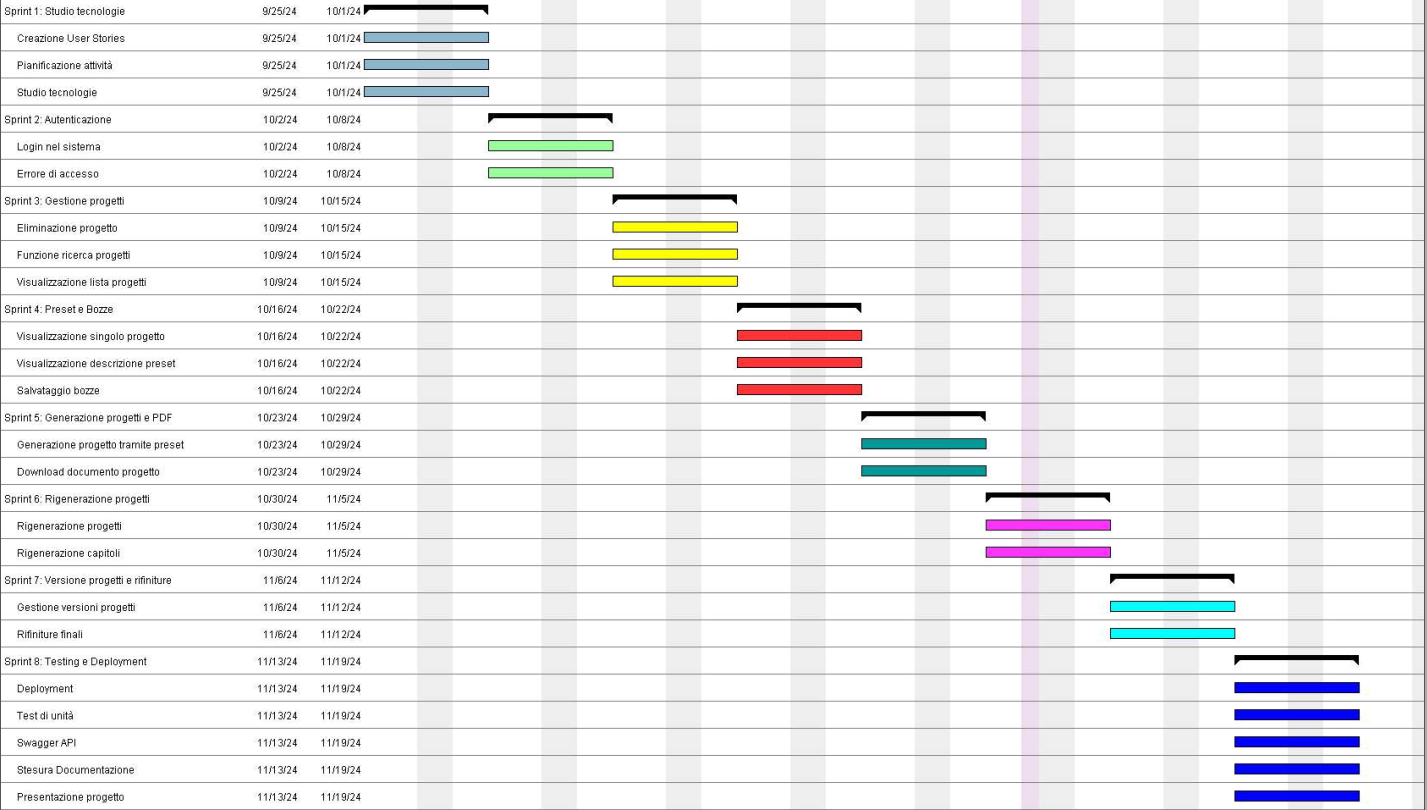
\includegraphics[scale=0.43]{pianificazione/gantt-chart.png}
    \caption{Diagramma di \textit{Gantt} delle attività svolte durante il periodo di stage}
    \label{fig:gantt-chart}
\end{figure}
%\pagebreak
\section{Analisi dei rischi}
\label{sez:analisi-dei-rischi}

L'analisi dei rischi è un'attività essenziale per identificare e gestire eventi incerti che potrebbero compromettere il successo del progetto. \\
Consiste nell’individuare i rischi, valutarne la probabilità e l’impatto, e pianificare strategie di mitigazione per ridurne gli effetti.\\

\noindent Per ogni rischio stilato nella {\hyperref[tab:analisi-rischi]{Tabella 3.1}} vengono definiti:

\begin{itemize}
    \item \textbf{Probabilità di occorrenza:} quanto è probabile che il rischio si verifichi (\textit{alta, media o bassa});
    \item \textbf{Descrizione:} una spiegazione del rischio e delle sue conseguenze;
    \item \textbf{Mitigazione:} azioni preventive o correttive per ridurre l’impatto.
\end{itemize}

\renewcommand{\arraystretch}{1.5} % Increases the row height for better vertical space

\begin{longtable}{|c|>{\centering\arraybackslash}p{0.7\textwidth}|} % Adjust the column width with p{0.7\textwidth}
    \hline
    \rowcolor{green!30} 
    \textbf{\#1} & \textbf{Inesperienza tecnologica} \\
    \hline
    \textbf{Occorrenza} & Alta \\
    \hline
    \textbf{Descrizione} & Lo stagista possiede poca esperienza con le tecnologie e gli strumenti principali necessari per il progetto, il che potrebbe rallentare lo sviluppo e compromettere la qualità delle soluzioni realizzate\\
    \hline
    \textbf{Mitigazione} & Prevedere una settimana iniziale dedicata all’autoformazione e all’approfondimento guidato delle tecnologie chiave. Durante questa fase, verranno forniti materiali di studio e accesso a risorse dedicate, con il supporto del \textit{tutor} aziendale per rispondere a eventuali dubbi e garantire un apprendimento efficace\\
    \hline

    \rowcolor{green!30} % Header color: light green
    \textbf{\#2} & \textbf{Inesperienza organizzativa} \\
    \hline
    \textbf{Occorrenza} & Media \\
    \hline
    \textbf{Descrizione} & Ridotta esperienza nella realizzazione di progetti utilizzando metodologie agili e nella gestione del lavoro per obiettivi. Questo potrebbe portare a inefficienze, difficoltà nel rispettare le scadenze e mancato raggiungimento degli obiettivi prefissati\\
    \hline
    \textbf{Mitigazione} & Fornire formazione iniziale sulle metodologie agili e affiancare una figura esperta per guidare lo stagista. Utilizzare strumenti di \textit{project management} per facilitare pianificazione e monitoraggio, organizzando retrospettive periodiche per migliorare il processo\\
    \hline
    \pagebreak

    \hline
    \rowcolor{green!30} % Header color: light green
    \textbf{\#3} & \textbf{Complessità del contesto di uso di servizi di \gls{generative-ai}} \\
    \hline
    \textbf{Occorrenza} & Alta \\
    \hline
    \textbf{Descrizione} & L’esperienza con i servizi di \gls{generative-ai} è limitata ad un contesto accademico e non è mai stata applicata in un progetto reale, aumentando il rischio di errori nella configurazione e integrazione\\
    \hline
    \textbf{Mitigazione} & Prevedere una fase iniziale dedicata allo studio della documentazione ufficiale dei servizi di \gls{generative-ai} utilizzati nel progetto, con approfondimenti su configurazione e integrazione. Integrare il percorso con il supporto di risorse esterne o \textit{community} online per risolvere eventuali problematiche tecniche\\
    \hline

    \rowcolor{green!30} % Header color: light green
    \textbf{\#4} & \textbf{Ridotta conoscenza dei servizi \textit{cloud} \gls{aws}} \\
    \hline
    \textbf{Occorrenza} & Media \\
    \hline
    \textbf{Descrizione} & Lo stagista ha una conoscenza limitata dei servizi \textit{cloud} \gls{aws}, il che potrebbe causare difficoltà nell’implementazione e gestione delle infrastrutture richieste\\
    \hline
    \textbf{Mitigazione} & Prevedere lo studio della documentazione ufficiale di \gls{aws} con particolare attenzione ai servizi rilevanti per il progetto. Affiancare questa attività con il supporto e l’aiuto di colleghi più esperti per chiarire dubbi e fornire indicazioni pratiche sull’utilizzo dei servizi\\
    \hline
    
    \rowcolor{green!30} % Header color: light green
    \textbf{\#5} & \textbf{Assenze per motivi di salute e/o personali} \\
    \hline
    \textbf{Occorrenza} & Bassa \\
    \hline
    \textbf{Descrizione} &  Lo stagista potrebbe dover affrontare assenze per motivi di salute o personali, con il rischio di rallentare l'avanzamento del progetto\\
    \hline
    \textbf{Mitigazione} &In caso di assenza programmata o imprevista, lo stagista dovrà avvisare tempestivamente il tutor aziendale. Questo permetterà di pianificare adeguatamente la gestione delle attività e delle scadenze, riducendo al minimo l'impatto sul progresso del progetto\\
    \hline

    \caption{Analisi dei rischi del progetto} % Table caption
    \label{tab:analisi-rischi} % Label for referencing the table
\end{longtable}
\pagebreak
\section{Analisi dei requisiti}
\label{sez:analisi-dei-requisiti}
L’analisi dei requisiti rappresenta una fase cruciale in qualsiasi progetto \textit{software}, poiché consente di definire in modo dettagliato e strutturato ciò che il sistema dovrà realizzare per soddisfare le necessità degli utenti e degli \textit{stakeholder}.\\
In questo progetto, l’analisi è stata condotta seguendo un approccio metodico che si è articolato in diverse fasi.\\

\noindent In primo luogo, ho effettuato una mappatura delle \gls{user-stories}, un processo che ha permesso di identificare le funzionalità principali richieste dagli utenti attraverso una rappresentazione visuale e iterativa. \\
Successivamente, ho individuato i casi d’uso, descrivendo in dettaglio gli scenari di interazione tra gli attori del sistema e le funzionalità del \textit{software}.\\
Infine, sulla base di queste informazioni, ho creato i \textit{requisiti}, formalizzando in modo chiaro e specifico ciò che il sistema deve implementare, suddividendo i requisiti in funzionali e non funzionali per garantire una visione completa del progetto.
\subsection{\textit{User Story Mapping}}
\label{subsec:user-story-mapping}

\subsection*{Introduzione}
\label{subsubsec:introduzione}

Le \gls{user-stories} rappresentano una tecnica fondamentale nel contesto dello sviluppo \textit{Agile}, in particolare all'interno del \textit{framework} \textit{Scrum}. \\
Questa metodologia consente di creare una visione d'insieme delle funzionalità richieste da un sistema, organizzandole in modo strutturato e collaborativo\footcite{site:user-stories}. \\

\noindent Lo \textit{User Story Mapping} è uno strumento visuale che suddivide il lavoro in componenti incrementali, aiutando il \textit{team} a comprendere il percorso del cliente e a pianificare il rilascio di valore progressivo.\\

\subsection*{Utilizzo nel contesto \textit{Scrum}}\\

\noindent Nel contesto di \textit{Scrum}, le \gls{user-stories} sono utilizzate per:

\begin{itemize}
    \item \textbf{Comprendere le esigenze degli utenti:} La mappatura aiuta a identificare le principali funzionalità del prodotto dal punto di vista degli utenti finali;
    \item \textbf{Definire un \textit{backlog} strutturato:} La tecnica consente di creare un \gls{product-backlog} organizzato, ordinando le \gls{user-stories} per priorità e obiettivi di rilascio;
    \item \textbf{Pianificare gli \gls{sprint}:} La mappa aiuta il \textit{Product Owner} ed il \textit{team} ad individuare le storie da completare in ciascun \gls{sprint}, bilanciando valore e complessità;
    \item \textbf{Favorire la collaborazione:} La mappa è creata in un incontro collaborativo che coinvolge il \textit{Product Owner}, il \textit{team} di sviluppo e, quando possibile, gli \textit{stakeholder}, per garantire un allineamento sulle priorità.
\end{itemize}

\pagebreak
\subsection*{Struttura delle \gls{user-stories}}\\

\noindent Ogni \textit{user story} segue una struttura standard che include diversi elementi essenziali:\\
\begin{itemize}

    \item \textbf{Priorità}, ogni storia viene classificata in base alla sua priorità, indicata con tre livelli derivati dal metodo \textit{MoSCoW}\footcite{site:moscow-method}:
    \begin{itemize}
        \item \textbf{M:} \textit{Must have} (essenziale): funzionalità indispensabili per il sistema;
        \item \textbf{S:} \textit{Should have} (importante): funzionalità utili ma non critiche;
        \item \textbf{C:} \textit{Could have} (opzionale): funzionalità che aggiungono valore ma possono essere escluse in caso di limitazioni temporali o di risorse.   
    \end{itemize}

    \item \textbf{Descrizione}, ogni storia è descritta in modo sintetico attraverso la notazione standard:

    \begin{center}
        Come [\textit{utente}], voglio [\textit{azione}], affinché [\textit{obiettivo}].
    \end{center}
    Ad esempio: "Come cliente, voglio visualizzare il catalogo prodotti, affinché possa scegliere cosa acquistare."\\

    \item \textbf{Criteri di accettazione}, questi definiscono le condizioni che devono essere soddisfatte affinché le \gls{user-stories} possano essere considerate completate.\\
    Sono specifiche misurabili che servono come riferimento per i \textit{test} e l’approvazione. \\

    \noindent Ad esempio, per la storia sopra, i criteri di accettazione potrebbero essere:

    \begin{itemize}
        \item Il catalogo deve mostrare almeno 20 prodotti per pagina;
        \item Ogni prodotto deve avere nome, immagine e prezzo visibili;
        \item L’utente deve poter filtrare i prodotti per categoria.
    \end{itemize}

\end{itemize}

\noindent Questa combinazione di priorità, descrizione e criteri di accettazione rende le \gls{user-stories} uno strumento potente per pianificare, monitorare e validare lo sviluppo di un progetto, assicurando che tutte le funzionalità siano orientate al valore per l’utente e il \textit{business}.

\pagebreak
\subsection*{\textit{Epic} e \textit{stories} identificate}
\label{subsubsec:epic-stories}

\vspace{0.5cm}
\section*{\textit{Epic} 1: Accesso alla piattaforma}

\subsection*{\textbf{M} - \textit{Login} nel sistema:}

\noindent Come utente voglio poter accedere al sistema e visualizzare la \textit{dashboard} così da gestire i miei progetti precedenti e crearne di nuovi. 

\subsubsection*{Criteri di accettazione:}

\begin{enumerate}
    \item L'utente deve poter accedere inserendo \textit{email} e \textit{password};
    \item In caso di credenziali corrette, l'utente deve essere reindirizzato alla \textit{dashboard} personale;
    \item Se le credenziali sono errate, deve essere mostrato un messaggio di errore appropriato;
    \item Il sistema deve rispettare le politiche di sicurezza, come il blocco temporaneo dopo tentativi falliti ripetuti.
\end{enumerate}

\vspace{0.5cm}

\subsection*{M - Errore di accesso in caso di credenziali errate:}

\noindent Come utente in caso di errore di accesso (es. \textit{password} errata), voglio essere informato con un messaggio chiaro su come risolvere il problema (ad es. come reimpostare la \textit{password}).

\subsubsection*{Criteri di accettazione:}

\begin{enumerate}
    \item Deve essere visualizzato un messaggio chiaro con istruzioni per risolvere il problema (ad esempio, come reimpostare la \textit{password});
    \item Il messaggio di errore non deve rivelare se l'\textit{email} esiste nel sistema per motivi di sicurezza.
\end{enumerate}

\vspace{0.5cm}
\subsection*{M - Piattaforma ottimizzata per \textit{mobile}:}

\noindent Come utente voglio poter accedere alla piattaforma \textit{web} tramite un'interfaccia \textit{mobile} ottimizzata così da poter gestire i miei progetti con facilità anche in mobilità.

\subsubsection*{Criteri di accettazione:}

\begin{enumerate}
    \item La piattaforma deve essere accessibile tramite \textit{browser mobile};
    \item Tutte le funzionalità chiave devono essere usabili su uno schermo \textit{mobile} senza problemi di \textit{layout} o navigazione.
\end{enumerate}

\vspace{0.5cm}

\subsection*{M - \textit{Logout }dal sistema:}

\noindent Come utente voglio avere la possibilità di disconnettermi dal sistema in modo semplice e rapido, così da garantire la sicurezza del mio \textit{account} e prevenire accessi non autorizzati.

\subsubsection*{Criteri di accettazione:}

\begin{enumerate}
    \item L'utente deve potersi disconnettere tramite un pulsante di \textit{logout} ben visibile;
    \item Dopo il \textit{logout}, l'utente deve essere reindirizzato alla pagina di \textit{login};
    \item La sessione dell'utente deve essere invalidata immediatamente.
\end{enumerate}

\vspace{0.5cm}

\section*{\textit{Epic} 2: Gestione dei Progetti}

\subsection*{S - Funzione ricerca e filtraggio progetti:}

\noindent Come utente voglio poter cercare e filtrare i miei progetti per data o nome così da trovare facilmente il progetto desiderato anche in un elenco molto lungo. 

\subsubsection*{Criteri di accettazione:}

\begin{enumerate}
    \item L'utente deve poter cercare i progetti per nome o data tramite un campo di ricerca;
    \item I risultati devono essere aggiornati dinamicamente durante la ricerca;
    \item I filtri devono includere opzioni per ordinare per data di creazione o nome.
\end{enumerate}

\vspace{0.5cm}

\subsection*{M - Visualizzazione singolo progetto}

\noindent Come utente voglio poter selezionare un singolo progetto salvato nella \textit{dashboard} così da visualizzarne i dettagli (nome, stato, data di creazione e le ultime modifiche) e poterlo rigenerare. 

\subsubsection*{Criteri di accettazione:}

\begin{enumerate}
    \item L'utente deve poter cliccare su un progetto dalla lista per accedere alla sua vista dettagliata;
    \item La pagina del progetto deve mostrare nome, stato, data di creazione e tutti i capitoli generati;
    \item Deve essere presente un'opzione per rigenerare il progetto dalla pagina di dettaglio dello stesso.
\end{enumerate}

\vspace{0.5cm}

\subsection*{M - Visualizzazione lista progetto:}

\noindent Come utente voglio poter vedere la lista di tutti i progetti precedentemente generati con annesso nome e data creazione, così da poter scegliere quale selezionare. 

\subsubsection*{Criteri di accettazione:}

\begin{enumerate}
    \item Tutti i progetti dell'utente devono essere visibili in una lista con nome e data di creazione:
    \item La lista deve essere scorrevole e ottimizzata per schermi di diverse dimensioni.
\end{enumerate}

\vspace{0.5cm}

\subsection*{M - Rigenerazione di un progetto:}

\noindent Come utente voglio poter rigenerare un progetto, aggiungendo o modificando informazioni, così da ottenere diverse versioni del documento per meglio adattarsi alle mie esigenze.

\subsubsection*{Criteri di accettazione:}

\begin{enumerate}
    \item L'utente deve poter accedere alla funzione di rigenerazione da un progetto esistente;
    \item Deve essere possibile inserire un \gls{prompt} contenente le direttive da usare per la rigenerazione del progetto;
    \item La versione rigenerata deve essere salvata come nuova versione del progetto.
\end{enumerate}

\vspace{0.5cm}

\subsection*{C - Visualizzazione versioni precedenti progetto:}

\noindent Come utente voglio poter visualizzare le versioni precedenti di un progetto così da poter ripristinare o confrontare modifiche, migliorando il controllo sulle evoluzioni del documento.

\subsubsection*{Criteri di accettazione:}

\begin{enumerate}
    \item L'utente deve poter visualizzare una lista cronologica delle versioni precedenti del progetto;
    \item Deve essere possibile selezionare e visualizzare una versione precedente.
\end{enumerate}

\vspace{0.5cm}
\pagebreak
\subsection*{S - Rigenerazione specifici capitoli}

\noindent Come utente voglio rigenerare specifici capitoli di un progetto già creato, mantenendo inalterati gli altri capitoli, così da aggiornare solo le sezioni che richiedono modifiche senza dover rigenerare tutto il documento.

\subsubsection*{Criteri di accettazione:}

\begin{enumerate}
    \item L'utente deve poter selezionare il capitolo da rigenerare dalla pagina di visualizzazione singolo progetto;
    \item Deve essere possibile inserire un \gls{prompt} contenente le direttive da usare per la rigenerazione del capitolo;
    \item La versione rigenerata deve essere salvata come nuova versione del progetto;
    \item I capitoli non selezionati devono rimanere invariati.
\end{enumerate}

\vspace{0.5cm}

\subsection*{C - Rimozione capitoli non necessari:}

\noindent Come utente voglio poter rimuovere singoli capitoli così da eliminare contenuti non necessari dal progetto. 

\subsubsection*{Criteri di accettazione:}

\begin{enumerate}
    \item L'utente deve poter selezionare e rimuovere i capitoli dal progetto;
    \item Prima della rimozione definitiva, deve essere mostrata una finestra di conferma.
\end{enumerate}

\vspace{0.5cm}

\subsection*{M - Eliminazione di un progetto:}

\noindent Come utente, voglio poter eliminare un progetto che ho creato in modo che possa rimuovere progetti non più necessari o irrilevanti.

\subsubsection*{Criteri di accettazione:}

\begin{enumerate}
    \item L'utente dalla pagina di visualizzazione singolo progetto deve poter richiedere l’eliminazione dello stesso;
    \item Deve essere mostrata una finestra di conferma prima dell'eliminazione definitiva del progetto;
    \item L'eliminazione deve rimuovere tutti i dati associati al progetto senza lasciare tracce;
    \item Se l'eliminazione è completata con successo, l'utente deve ricevere una notifica di conferma.
\end{enumerate}

\vspace{0.5cm}

\section*{\textit{Epic} 3: Creazione di nuovi progetti}

\subsection*{M - Generazione progetto tramite \textit{preset}:}

\noindent Come utente voglio poter generare un progetto con l'aiuto di \textit{preset} predefiniti e ottimizzati, così da creare rapidamente un documento utile e strutturato senza partire da zero.

\subsubsection*{Criteri di accettazione:}

\begin{enumerate}
    \item All’interno della pagina di creazione di un progetto l'utente deve poter selezionare un \textit{preset} predefinito dalla lista;
    \item Dopo la selezione e la compilazione del \textit{preset} il progetto deve essere generato con i dati inseriti;
    \item Se la generazione avviene con successo, l’utente viene reindirizzato alla pagina di visualizzazione del singolo progetto;
    \item L’utente riceve una notifica di successo.
\end{enumerate}

\vspace{0.5cm}

\subsection*{M - Visualizzazione descrizione \textit{preset}:}

\noindent Come utente voglio visualizzare una descrizione dettagliata di ciascun \textit{preset} così da scegliere quello più adatto alle mie esigenze specifiche.

\subsubsection*{Criteri di accettazione:}

\begin{enumerate}
    \item Ogni \textit{preset} deve avere una descrizione dettagliata visibile prima della selezione;
    \item La descrizione deve includere le caratteristiche e i casi d'uso principali del \textit{preset}.
\end{enumerate}

\vspace{0.5cm}

\subsection*{S - Salvataggio \textit{preset} compilato:}

\noindent Come utente voglio poter salvare il \textit{preset} compilato così da poterlo completare e generare il documento in un momento successivo.

\subsubsection*{Criteri di accettazione:}

\begin{enumerate}
    \item L'utente deve poter salvare un \textit{preset} (parzialmente) compilato per completarlo in un secondo momento;
    \item Il sistema deve indicare chiaramente che il \textit{preset} è salvato in bozza.
\end{enumerate}

\vspace{0.5cm}

\pagebreak
\subsection*{C - Personalizzazione campi \textit{preset}:}

\noindent Come utente voglio personalizzare i campi del \textit{preset} così da adattarlo alle mie specifiche necessità e rendere unico il progetto. 

\subsubsection*{Criteri di accettazione:}

\begin{enumerate}
    \item L'utente deve poter modificare i campi predefiniti del \textit{preset};
    \item Le modifiche devono essere salvate, rendendo possibile l’utilizzo del \textit{preset} personalizzato in secondo momento
\end{enumerate}

\vspace{0.5cm}

\subsection*{C - Generazione progetto senza \textit{preset}:}

\noindent Come utente voglio poter generare un progetto senza l’utilizzo di un \textit{preset} così da avere il massimo controllo e flessibilità sulla struttura del documento finale, migliorando la personalizzazione per casi d'uso complessi. 

\subsubsection*{Criteri di accettazione:}

\begin{enumerate}
    \item L'utente deve poter generare un nuovo progetto senza scegliere un \textit{preset};
    \item Deve essere possibile inserire un prompt contenente le direttive da usare per la generazione del progetto.
\end{enumerate}

\vspace{0.5cm}

\subsection*{M - Download documento progetto:}

\noindent Come utente voglio poter scaricare il progetto generato in formato PDF così da poterlo condividere facilmente con il mio \textit{team} o archiviare per un utilizzo futuro.

\subsubsection*{Criteri di accettazione:}

\begin{enumerate}
    \item Dalla pagina di visualizzazione singolo progetto l'utente deve poter scaricare il progetto in formato PDF;
    \item Il \textit{file} generato deve includere tutti i capitoli del progetto.
\end{enumerate}

\vspace{0.5cm}

\subsection*{S - Generazione progetto tramite diversi \gls{llm}:}

\noindent Come utente voglio poter scegliere tra vari \gls{llm} per la generazione del progetto così da avere varie maggiore scelta (progetti più grandi vs. progetti più piccoli). 

\subsubsection*{Criteri di accettazione:}

\begin{enumerate}
    \item L'utente deve poter selezionare tra una lista di \gls{llm} disponibili prima della generazione del progetto;
    \item Ogni modello deve avere una descrizione che ne spiega le capacità ed i casi d'uso.
\end{enumerate}

\vspace{0.5cm}

\section*{\textit{Epic} 4: Piattaforma amministratore}

\subsection*{C - Aggiunta nuovo \textit{preset}:}

\noindent Come amministratore voglio poter aggiungere un nuovo \textit{preset} così da poter dare maggior scelta nella creazione di progetti agli utenti.

\subsubsection*{Criteri di accettazione:}

\begin{enumerate}
    \item L'amministratore deve poter accedere a un modulo per creare un nuovo \textit{preset};
    \item Il \textit{preset} aggiunto deve essere visibile agli utenti finali immediatamente dopo il salvataggio.
\end{enumerate}

\vspace{0.5cm}

\subsection*{C - Modifica \textit{preset} esistente:}

\noindent Come amministratore voglio poter modificare un \textit{preset} già esistente, così da poterlo migliorare e aggiornare nel tempo o non renderlo più disponibile all’utilizzo da parte degli utenti.

\subsubsection*{Criteri di accettazione:}

\begin{enumerate}
    \item L'amministratore deve poter modificare nome, descrizione e campi di un \textit{preset} esistente;
    \item Le modifiche devono essere salvate e applicate ai nuovi progetti creati con quel \textit{preset}.
\end{enumerate}

\vspace{0.5cm}

\subsection*{C - Eliminazione \textit{preset} esistente:}

\noindent Come amministratore voglio poter eliminare un \textit{preset} già esistente così da poter eliminare \textit{preset} poco utilizzati o obsoleti.

\begin{enumerate}
    \item L'amministratore deve poter eliminare un \textit{preset} selezionato;
    \item Deve essere mostrata una finestra di conferma prima della rimozione definitiva.
\end{enumerate}

\vspace{0.5cm}

\subsection*{C - Gestione \gls{llm}:}

\noindent Come amministratore voglio poter aggiungere o rimuovere l’accesso agli utenti ad una \gls{llm}, così da poter eliminare \gls{llm} obsolete o aggiungerne di nuove maggiormente performanti.

\subsubsection*{Criteri di accettazione:}

\begin{enumerate}
    \item L'amministratore deve poter aggiungere nuovi modelli \gls{llm} alla piattaforma;
    \item Deve essere possibile rimuovere i modelli \gls{llm} non più utilizzati.
\end{enumerate}

\subsection{Casi d'uso}
\label{subsec:casi-duso}

I diagrammi dei casi d’uso consentono di descrivere in modo chiaro e strutturato le interazioni tra gli attori e il sistema.\\

\noindent Per la stesura dei casi d’uso, ho adottato una convenzione specifica, organizzata come segue:

\begin{center}
\textbf{UC[Numero] - Nome del caso d’uso}
\end{center}

Dove:
\begin{itemize}
    \item \textbf{UC}: acronimo di \textit{Use Case};
    \item \textbf{Numero}: identificatore progressivo del caso d’uso.\\
    I sottocasi sono rappresentati nella forma [Numero].[SottoNumero].
\end{itemize}

\noindent Ogni caso d’uso è corredato da una descrizione dettagliata, dalla lista degli attori coinvolti, dalla sua descrizione, dalle precondizioni e dalle postcondizioni necessarie affinché il caso d’uso possa essere eseguito correttamente.\\

\noindent Per supportare la comprensione dei casi d’uso, sono stati realizzati dei diagrammi \gls{uml}, che forniscono una rappresentazione grafica degli scenari. \\
Ho inlcuso esclusivamente i diagrammi relativi ai casi d’uso principali, omettendo quelli banali o secondari per privilegiare chiarezza e rilevanza.\\

\noindent Questa metodologia garantisce un’organizzazione chiara e coerente dei casi d’uso, facilitando la comprensione e la condivisione tra i vari stakeholder coinvolti nel progetto.

\subsubsection{Attori}
\label{subsubsec:attori}

Nel contesto dei casi d'uso, un attore è colui che interagisce con il sistema per ottenere un obiettivo specifico.\\
Uno schema contenente tutti gli attori è visibile in {\hyperref[fig:attori-casi-duso]{Figura 3.2}}, mentre i dettagli di ciascun attore sono descritti di seguito:

\subsection*{Utente non autenticato:}

\begin{itemize}
    \item \textbf{Descrizione:}  L'utente non autenticato è una persona che sta cercando di accedere al sistema, ma non ha effettuato il \textit{login}.\\
    Non ha accesso ai dati sensibili o alle funzionalità avanzate riservate agli utenti autenticati;
    \item \textbf{Ruolo:} Questo attore ha il compito di interagire con il sistema senza diritti di accesso completi.\\
    Il suo obiettivo principale è autenticarsi per diventare un utente con pieno accesso al sistema;
    \item \textbf{Attività principali:}
        \begin{itemize}
            \item Effettuare il \textit{login} con le proprie credenziali;
            \item Visualizzare i messaggi di errore in caso di \textit{login} fallito.
        \end{itemize}
\end{itemize}

\subsection*{Utente autenticato:}

\begin{itemize}
    \item \textbf{Descrizione:}  L'utente autenticato è una persona che ha effettuato il \textit{login} con successo ed ha accesso completo alle funzionalità del sistema.\\
    Può cercare, filtrare, visualizzare, generare e rigenerare i progetti;
    \item \textbf{Ruolo:} Questo attore può eseguire operazioni avanzate, come la generazione di progetti, il salvataggio delle bozze ed il \textit{download} dei progetti in formato PDF;
    \item \textbf{Attività principali:}
        \begin{itemize}
            \item Visualizzare e cercare progetti;
            \item Generare e rigenerare progetti;
            \item Salvare e visualizzare bozze;
            \item Visualizzare e scaricare progetti in formato PDF.
        \end{itemize}
\end{itemize}

\subsection*{\textit{Large language models}:}

\begin{itemize}
    \item \textbf{Descrizione:}  L'attore \gls{llm} è un sistema automatizzato di generazione dei contenuti, che utilizza algoritmi avanzati di \gls{aig} per generare e rigenerare progetti o singoli capitoli di progetti. \\
    Il \gls{llm} è responsabile dell'elaborazione delle richieste degli utenti e della generazione automatica del contenuto tecnico dei progetti;
    \item \textbf{Ruolo:}  Il \gls{llm} è un componente del sistema che esegue la generazione di contenuti complessi in modo autonomo.\\
    La sua funzione principale è rispondere alle richieste dell'utente riguardo la creazione e la rigenerazione di progetti;
    \item \textbf{Attività principali:}
        \begin{itemize}
            \item Ricevere richieste di generazione di progetti da parte degli utenti;
            \item Generare contenuti basati su preset predefiniti;
            \item Rigenerare progetti o singoli capitoli in risposta a richieste di aggiornamento;
            \item Restituire i contenuti generati all'utente.
        \end{itemize}
\end{itemize}

\begin{figure}[H]
    \centering
    
\includegraphics[width=1\textwidth]{usecase/attori.png}
    \caption{Attori dei casi d'uso}
    \label{fig:attori-casi-duso}
\end{figure}




\pagebreak
\subsubsection{Casi d'uso individuati}
\label{subsubsec:casi-uso-individuati}

\section*{UC1 - \textit{Login} dell'utente}

\begin{figure}[H]
    \centering
    
\includegraphics[scale=0.5]{usecase/uc1.png}
    \caption{UC1 - \textit{Login} dell'utente}
    \label{fig:uc1}
\end{figure}
\begin{itemize}
    \item \textbf{Attori}: Utente non autenticato;
    \item \textbf{Descrizione}: L'utente inserisce le proprie credenziali per accedere al sistema;
    \item \textbf{Precondizioni}: L'utente non è autenticato nel sistema;
    \item \textbf{Postcondizioni}: L'utente viene autenticato e reindirizzato alla \textit{dashboard} del sistema;
    \item \textbf{Flusso principale}:
    \begin{enumerate}
        \item L'utente naviga alla pagina di \textit{login};
        \item L'utente inserisce \textit{email} e \textit{password};
        \item Il sistema verifica le credenziali;
        \item Se le credenziali sono corrette, l'utente viene autenticato e reindirizzato alla \textit{dashboard}.
    \end{enumerate}
    \item \textbf{Estensioni}: UC3 - Visualizzazione errore in caso di \textit{login} non riuscito
\end{itemize}

\vspace{0.5cm}
\section*{UC2 - \textit{Logout} dell'utente}
\begin{itemize}
    \item \textbf{Attori}: Utente autenticato;
    \item \textbf{Descrizione}: L'utente può disconnettersi dal sistema;
    \item \textbf{Precondizioni}: L'utente è autenticato;
    \item \textbf{Postcondizioni}: L'utente viene disconnesso e reindirizzato alla pagina di \textit{login};
    \item \textbf{Flusso principale}:
    \begin{enumerate}
        \item L'utente clicca sul pulsante di \textit{logout};
        \item L'utente conferma la volontà di effettuare il \textit{logout};
        \item Il sistema disconnette l'utente;
        \item L'utente viene reindirizzato alla pagina di \textit{login}.
    \end{enumerate}
\end{itemize}

\vspace{0.5cm}
\section*{UC3 - Visualizzazione errore in caso di \textit{login} non riuscito}
\begin{itemize}
    \item \textbf{Attori}: Utente non autenticato;
    \item \textbf{Descrizione}: L'utente visualizza un messaggio di errore quando il \textit{login} fallisce;
    \item \textbf{Precondizioni}: L'utente ha inserito credenziali errate;
    \item \textbf{Postcondizioni}: Un messaggio di errore viene mostrato all'utente;
    \item \textbf{Flusso principale}:
    \begin{enumerate}
        \item L'utente inserisce credenziali errate;
        \item Il sistema verifica le credenziali;
        \item Il sistema visualizza un messaggio di errore indicando che il \textit{login} è fallito.
    \end{enumerate}
\end{itemize}

\vspace{0.5cm}  
\section*{UC4 - Visualizzazione lista progetti}
\begin{itemize}
    \item \textbf{Attori}: Utente autenticato;
    \item \textbf{Descrizione}: L'utente visualizza la lista di tutti i progetti disponibili;
    \item \textbf{Precondizioni}: L'utente è autenticato;
    \item \textbf{Postcondizioni}: La lista di progetti viene visualizzata;
    \item \textbf{Flusso principale}:
    \begin{enumerate}
        \item L'utente accede alla \textit{dashboard} del sistema;
        \item Il sistema recupera e visualizza la lista di tutti i progetti disponibili;
        \item L'utente può vedere il nome, la data di creazione ed il preset usato per la generazione dei progetti.
    \end{enumerate}
\end{itemize}

\vspace{0.5cm}  
\section*{UC5 - Ricerca e filtraggio dei progetti}
\begin{itemize}
    \item \textbf{Attori}: Utente autenticato;
    \item \textbf{Descrizione}: L'utente cerca e filtra i progetti utilizzando specifici criteri;
    \item \textbf{Precondizioni}: L'utente è autenticato e si trova nella dashboard di sistema;
    \item \textbf{Postcondizioni}: I progetti che soddisfano i criteri di ricerca e/o filtro vengono visualizzati;
    \item \textbf{Flusso principale}:
    \begin{enumerate}
        \item L'utente inserisce parole chiave e/o seleziona i filtri;
        \item Il sistema applica i filtri e visualizza i progetti corrispondenti.
    \end{enumerate}
\end{itemize}

\vspace{0.5cm}  
\section*{UC6 - Visualizzazione dei dettagli di un progetto singolo}
\begin{itemize}
    \item \textbf{Attori}: Utente autenticato;
    \item \textbf{Descrizione}: L'utente visualizza i dettagli di un progetto specifico selezionato dalla lista dei progetti;
    \item \textbf{Precondizioni}: 
    \begin{itemize}
        \item L'utente è autenticato;
        \item Il progetto selezionato è stato precedentemente creato dall'utente.
    \end{itemize}
    \item \textbf{Postcondizioni}: Il sistema mostra i dettagli del progetto selezionato, inclusi nome, descrizione, data di creazione, e tutti i capitoli che lo compongono;
    \item \textbf{Flusso principale}:
    \begin{enumerate}
        \item L'utente accede alla lista dei progetti salvati;
        \item L'utente seleziona un progetto dalla lista;
        \item Il sistema recupera i dati del progetto selezionato dal \textit{database};
        \item Il sistema mostra i dettagli del progetto in una pagina dedicata, inclusi:
        \begin{itemize}
            \item Nome del progetto;
            \item Descrizione del progetto;
            \item Data di creazione;
            \item Sezioni e contenuti specifici del progetto.
        \end{itemize}
    \end{enumerate}
\end{itemize}

\vspace{0.5cm}  
\section*{UC7 - Visualizzazione descrizione \textit{preset}}
\begin{itemize}
    \item \textbf{Attori}: Utente autenticato;
    \item \textbf{Descrizione}: L'utente visualizza la descrizione di un \textit{preset} disponibile;
    \item \textbf{Precondizioni}: L'utente è autenticato;
    \item \textbf{Postcondizioni}: La descrizione del \textit{preset} viene visualizzata;
    \item \textbf{Flusso principale}:
    \begin{enumerate}
        \item L’utente naviga nella pagina di creazione di un progetto;
        \item L'utente seleziona un \textit{preset} dalla lista di quelli disponibili;
        \item Il sistema visualizza la descrizione dettagliata del \textit{preset}.
    \end{enumerate}
\end{itemize}

\vspace{0.5cm}  
\section*{UC8 - Salvataggio di un \textit{preset} compilato}
\begin{itemize}
    \item \textbf{Attori}: Utente autenticato;
    \item \textbf{Descrizione}: L'utente salva un \textit{preset} parzialmente compilato come bozza;
    \item \textbf{Precondizioni}: L'utente è autenticato e deve aver iniziato a compilare un \textit{preset};
    \item \textbf{Postcondizioni}: Il \textit{preset} parzialmente compilato viene salvato come bozza;
    \item \textbf{Flusso principale}:
    \begin{enumerate}
        \item L'utente compila una parte del \textit{preset};
        \item L'utente clicca su "Salva bozza";
        \item Il sistema salva la bozza del \textit{preset} nel \textit{database}.
    \end{enumerate}
\end{itemize}

\vspace{0.5cm}  
\section*{UC9 - Visualizzazione lista bozze}
\begin{itemize}
    \item \textbf{Attori}: Utente autenticato;
    \item \textbf{Descrizione}: L'utente visualizza la lista di tutte le bozze disponibili;
    \item \textbf{Precondizioni}: L'utente è autenticato;
    \item \textbf{Postcondizioni}: La lista di bozze viene visualizzata;
    \item \textbf{Flusso principale}:
    \begin{enumerate}
        \item L'utente accede alla \textit{dashboard} del sistema;
        \item L'utente seleziona il pulsante di visualizzazione della lista di bozze;
        \item Il sistema recupera e visualizza la lista di tutte le bozze disponibili;
        \item L'utente può vedere il nome, la data di creazione ed il preset utilizzato per ogni bozza.
    \end{enumerate}
\end{itemize}

\vspace{0.5cm}  
\section*{UC10 - Ricerca e filtraggio delle bozze}
\begin{itemize}
    \item \textbf{Attori}: Utente autenticato;
    \item \textbf{Descrizione}: L'utente cerca e filtra le bozze utilizzando specifici criteri;
    \item \textbf{Precondizioni}: 
    \begin{itemize}
        \item L'utente è autenticato;
        \item L'utente si trova nella \textit{dashboard} di sistema ed ha selezionato il pulsante di visualizzazione della lista di bozze.
    \end{itemize}
    \item \textbf{Postcondizioni}: Le bozze che soddisfano i criteri di ricerca e/o filtro vengono visualizzate;
    \item \textbf{Flusso principale}:
    \begin{enumerate}
        \item L'utente inserisce parole chiave e/o seleziona i filtri;
        \item Il sistema applica i filtri e visualizza le bozze corrispondenti.
    \end{enumerate}
\end{itemize}

\vspace{0.5cm}  
\section*{UC11 - Generazione di un progetto}
\begin{figure}[H]
    \centering
    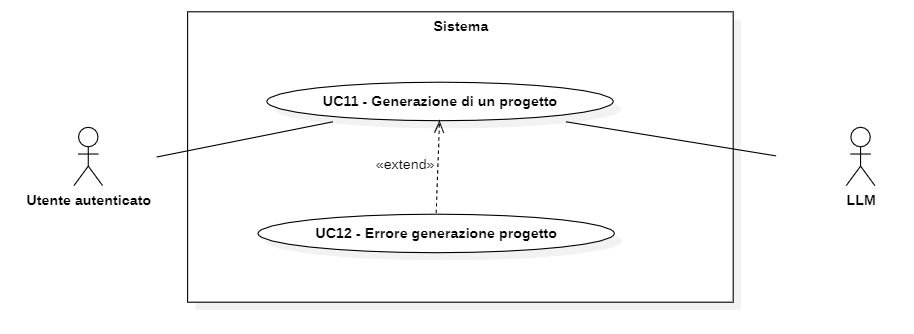
\includegraphics[scale=0.6]{usecase/uc11.png}
    \caption{UC11 - Generazione di un progetto}
    \label{fig:uc11}
\end{figure}
\begin{itemize}
    \item \textbf{Attori}: Utente autenticato, \gls{llm};
    \item \textbf{Descrizione}: L'utente avvia la generazione di un progetto utilizzando un \textit{preset};
    \item \textbf{Precondizioni}: 
    \begin{itemize}
        \item L'utente è autenticato;
        \item L'utente si trova nella pagina di creazione di un progetto ed ha selezionato un \textit{preset}.
    \end{itemize}
    \item \textbf{Postcondizioni}: Il progetto viene generato e l'utente vede le informazioni generate;
    \item \textbf{Flusso principale}:
    \begin{enumerate}
        \item L'utente compila nella sua interezza il \textit{preset} selezionato;
        \item L'utente richiede la generazione del progetto;
        \item Il sistema invia la richiesta al \gls{llm};
        \item Il \gls{llm} elabora la richiesta e genera il progetto;
        \item L'utente viene reindirizzato alla pagina di visualizzazione del progetto.
    \end{enumerate}
    \item \textbf{Estensioni}: UC12 - Visualizzazione errore generazione progetto
\end{itemize}

\vspace{0.5cm}
\section*{UC12 - Visualizzazione errore generazione progetto}
\begin{itemize}
    \item \textbf{Attori}: Utente autenticato;
    \item \textbf{Descrizione}: L'utente visualizza un messaggio di errore la generazione del progetto fallisce;
    \item \textbf{Precondizioni}: L'utente sta generando un progetto;
    \item \textbf{Postcondizioni}: Un messaggio di errore viene mostrato all'utente;
    \item \textbf{Flusso principale}:
    \begin{enumerate}
        \item L'utente invia la richiesta all'\gls{llm} per la generazione del progetto;
        \item \gls{llm} non riesce a generare il progetto richiesto;
        \item Il sistema visualizza un messaggio di errore indicando che la generazione del progetto è fallita.
    \end{enumerate}
\end{itemize}

\vspace{0.5cm}  
\section*{UC13 - Rigenerazione completa di un progetto}
\begin{figure}[H]
    \centering
    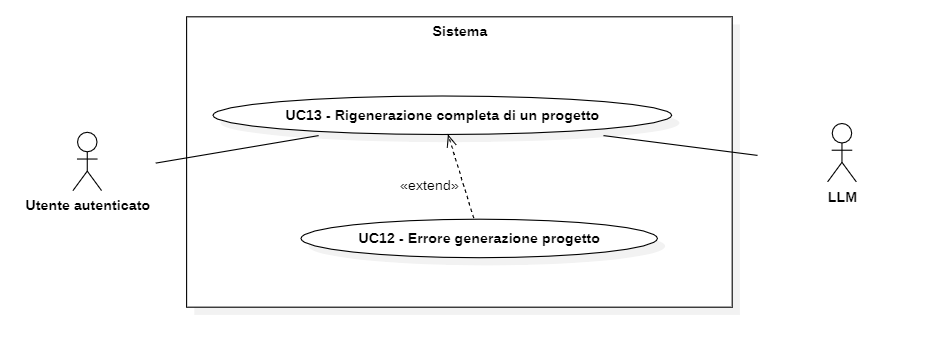
\includegraphics[scale=0.6]{usecase/uc13.png}
    \caption{UC13 - Rigenerazione completa di un progetto}
    \label{fig:uc13}
\end{figure}
\begin{itemize}
    \item \textbf{Attori}: Utente autenticato, \gls{llm};
    \item \textbf{Descrizione}: L'utente rigenera un intero progetto, sostituendo completamente il contenuto esistente;
    \item \textbf{Precondizioni}: 
    \begin{itemize}
        \item L'utente è autenticato;
        \item L'utente si trova nella pagina di visualizzazione del singolo progetto.
    \end{itemize}
    \item \textbf{Postcondizioni}: Il progetto viene completamente rigenerato;
    \item \textbf{Flusso principale}:
    \begin{enumerate}
        \item L'utente seleziona il pulsante di rigenerazione completa del progetto;
        \item Il sistema richiede all'utente l'inserimento di un prompt su cui si baserà la rigenerazione;
        \item L'utente richiede la rigenerazione del progetto;
        \item Il sistema invia la richiesta di rigenerazione al \gls{llm};
        \item Il \gls{llm} rigenera completamente il progetto;
        \item Il progetto rigenerato viene visualizzato all'utente.
    \end{enumerate}
    \item \textbf{Estensioni}: UC12 - Visualizzazione errore generazione progetto
\end{itemize}

\vspace{0.5cm}  
\section*{UC14 - Rigenerazione di un singolo capitolo di un progetto}
\begin{figure}[H]
    \centering
    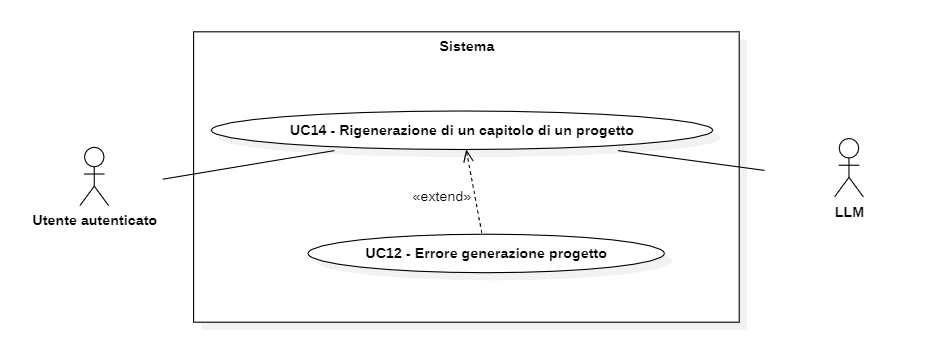
\includegraphics[scale=0.6]{usecase/uc14.png}
    \caption{UC14 - Rigenerazione di un singolo capitolo di un progetto}
    \label{fig:uc14}
\end{figure}
\begin{itemize}
    \item \textbf{Attori}: Utente autenticato, \gls{llm};
    \item \textbf{Descrizione}: L'utente rigenera un singolo capitolo del progetto, lasciando invariato il resto del progetto;
    \item \textbf{Precondizioni}: L'utente è autenticato e si trova nella pagina di visualizzazione del singolo progetto;
    \item \textbf{Postcondizioni}: Il capitolo selezionato viene rigenerato;
    \item \textbf{Flusso principale}:
    \begin{enumerate}
        \item L'utente seleziona il capitolo da rigenerare;
        \item Il sistema richiede all’utente l’inserimento di un \textit{prompt} su cui si baserà la rigenerazione;
        \item L’utente richiede la rigenerazione del capitolo;
        \item Il sistema invia la richiesta di rigenerazione al \gls{llm} per il capitolo selezionato;
        \item Il \gls{llm} rigenera solo il capitolo selezionato;
        \item Il progetto rigenerato viene visualizzato all'utente.
    \end{enumerate}
    \item \textbf{Estensioni}: UC12 - Visualizzazione errore generazione progetto
\end{itemize}

\vspace{0.5cm}  
\section*{UC15 - Eliminazione di un progetto}
\begin{itemize}
    \item \textbf{Attori}: Utente autenticato;
    \item \textbf{Descrizione}: L'utente elimina un progetto esistente;
    \item \textbf{Precondizioni}: L'utente è autenticato e si trova nella pagina di visualizzazione del singolo progetto;
    \item \textbf{Postcondizioni}: Il progetto viene eliminato dal sistema;
    \item \textbf{Flusso principale}:
    \begin{enumerate}
        \item L'utente seleziona il pulsante per l’eliminazione del progetto;
        \item L'utente conferma l'eliminazione del progetto;
        \item Il sistema elimina il progetto dal \textit{database}.
    \end{enumerate}
\end{itemize}

\vspace{0.5cm}  
\section*{UC16 - Visualizzazione del progetto in formato PDF}
\begin{itemize}
    \item \textbf{Attori}: Utente autenticato;
    \item \textbf{Descrizione}: L'utente visualizza il progetto generato in formato PDF;
    \item \textbf{Precondizioni}: L'utente è autenticato e si trova nella pagina di visualizzazione del singolo progetto;
    \item \textbf{Postcondizioni}: Il progetto viene visualizzato come PDF;
    \item \textbf{Flusso principale}:
    \begin{enumerate}
        \item L'utente seleziona il pulsante di visualizzazione del progetto in formato PDF;
        \item Il sistema mostra il progetto in formato PDF.
    \end{enumerate}
\end{itemize}

\vspace{0.5cm}  
\section*{UC17 - \textit{Download} del progetto in formato PDF}
\begin{itemize}
    \item \textbf{Attori}: Utente autenticato;
    \item \textbf{Descrizione}: L'utente scarica il progetto in formato PDF;
    \item \textbf{Precondizioni}: L’utente si trova nella pagina di visualizzazione del singolo progetto ed ha selezionato il pulsante di visualizzazione del PDF;
    \item \textbf{Postcondizioni}: Il progetto in formato PDF viene scaricato nel dispositivo dell'utente;
    \item \textbf{Flusso principale}:
    \begin{enumerate}
        \item L’utente seleziona il pulsante di \textit{download} del progetto in formato PDF;
        \item L'utente scarica il progetto in formato PDF.
    \end{enumerate}
\end{itemize}

\vspace{0.5cm}  
\section*{UC18 - Visualizzazione delle versioni precedenti di un progetto}
\begin{itemize}
    \item \textbf{Attori}: Utente autenticato;
    \item \textbf{Descrizione}: L'utente visualizza una lista delle versioni precedenti di un progetto selezionato e può accedere ai dettagli di una specifica versione;
    \item \textbf{Precondizioni}: L'utente è autenticato e il progetto selezionato ha almeno due versioni salvate;
    \item \textbf{Postcondizioni}: 
    \begin{itemize}
        \item Il sistema mostra la lista delle versioni precedenti del progetto, inclusi dettagli come numero di versione e data di creazione;
        \item L'utente può selezionare una versione specifica e visualizzarne i dettagli.
    \end{itemize}
    \item \textbf{Flusso principale}:
    \begin{enumerate}
        \item L'utente accede alla pagina dei dettagli di un progetto;
        \item L'utente seleziona la versione del progetto;
        \item Il sistema recupera e mostra una lista delle versioni precedenti del progetto, con i seguenti dettagli:
        \begin{itemize}
            \item Numero di versione;
            \item Data di creazione.
        \end{itemize}
        \item L'utente seleziona una specifica versione dalla lista;
        \item Il sistema mostra i dettagli della versione selezionata, inclusi i contenuti del progetto in quella versione.
    \end{enumerate}
\end{itemize}

\vspace{0.5cm}  
\section*{UC19 - Rimozione di capitoli non necessari da un progetto}
\begin{itemize}
    \item \textbf{Attori}: Utente autenticato;
    \item \textbf{Descrizione}: L'utente rimuove uno o più capitoli non necessari da un progetto per semplificarne la struttura o adattarlo a nuove esigenze;
    \item \textbf{Precondizioni}: 
    \begin{itemize}
        \item L'utente è autenticato;
        \item Il progetto contiene capitoli modificabili o rimovibili.
    \end{itemize}
    \item \textbf{Postcondizioni}: 
    \begin{itemize}
        \item Il sistema aggiorna la struttura del progetto eliminando i capitoli selezionati;
        \item La versione aggiornata del progetto è salvata nel sistema.
    \end{itemize}
    \item \textbf{Flusso principale}:
    \begin{enumerate}
        \item L'utente accede alla pagina di visualizzazione di un progetto;
        \item L'utente seleziona l'opzione "Gestione capitoli";
        \item Il sistema mostra la lista dei capitoli attualmente presenti nel progetto;
        \item L'utente seleziona uno o più capitoli che desidera rimuovere;
        \item L'utente conferma l'operazione di rimozione;
        \item Il sistema elimina i capitoli selezionati e aggiorna il progetto.
    \end{enumerate}
\end{itemize}

\subsection{Tracciamento dei requisiti}
\label{subsec:requisiti}

Lista dei requisiti individuati, con spiegazione della notazione utilizzata e classificazione tra requisiti funzionali e non funzionali, obbligatori, desiderabili e facoltativi.\\
\section{Progettazione}
\label{sez:progettazione}
 
\subsection{Architettura del sistema}
\label{subsec:architettura}

Per il progetto ho adottato un'architettura a livelli, nota come \textit{Three-Tier Architecture}, questa architettura è composta da tre livelli distinti:

\begin{itemize}
    \item \textbf{\textit{Presentation Tier}}: rappresenta il livello di interfaccia utente (\gls{ui}) del sistema,
    che si occupa di ricevere \textit{input} dall'utente e di visualizzare i risultati forniti dal livello logico;
    
    \item \textbf{\textit{Logic Tier}}: o livello logico, è il cuore del sistema,
    che si occupa di elaborare i dati, applicare la logica di \textit{business} e gestire le richieste provenienti dal \textit{Presentation Tier};
    
    \item \textbf{\textit{Data Tier}}: gestisce la persistenza dei dati del sistema, garantendo la loro memorizzazione, recupero e integrità.
\end{itemize}

\subsubsection{Motivazione della scelta}

\noindent Ho scelto di adottare un'architettura a livelli in quanto rappresenta una soluzione versatile e strutturata, ideale per gestire la complessità dei sistemi moderni. \\
Questa scelta favorisce un'organizzazione chiara e coerente, permettendo di ottimizzare lo sviluppo e la gestione del progetto nel tempo.

\noindent Di seguito, analizzo i principali vantaggi e svantaggi di questa architettura, evidenziandone l'impatto sull'efficienza e sulla scalabilità del sistema.
\pagebreak
\subsubsection{Vantaggi}
\begin{itemize}
    \item \textbf{Modularità}: Ogni livello è indipendente e può essere sviluppato, testato e manutenuto separatamente;
    \item \textbf{Scalabilità}: È possibile scalare ogni livello in modo indipendente, ottimizzando le risorse in base alle esigenze;
    \item \textbf{Manutenibilità}: La separazione delle responsabilità semplifica la risoluzione dei problemi e l'implementazione di nuove funzionalità;
    \item \textbf{Riutilizzabilità}: I moduli di ogni livello possono essere riutilizzati in altri progetti con minime modifiche.
\end{itemize}

\subsubsection{Svantaggi}
\begin{itemize}
    \item \textbf{Maggiore complessità}: L'implementazione e il coordinamento di più livelli richiedono un maggiore sforzo di progettazione;
    \item \textbf{\textit{Overhead} di comunicazione}: La comunicazione tra i livelli può introdurre un'inevitabile latenza;
    \item \textbf{Dipendenze tecnologiche}: Ogni livello richiede competenze specifiche nelle tecnologie utilizzate.
\end{itemize}

\subsubsection{Comunicazione tra i livelli}

\noindent Ho implementato la comunicazione tra i livelli tramite protocolli standard e strumenti specifici:
\begin{itemize}
    \item Tra il \textit{Presentation Tier} e il \textit{Logic Tier}, la comunicazione avviene tramite \gls{api-restful}, che permettono lo scambio di dati in formato \textit{JSON};
    \item Tra il \textit{Logic Tier} e il \textit{Data Tier}, è stato utilizzato l'\gls{odm} \textit{Mongoose}, che facilita l'interazione con \textit{MongoDB}, permettendo di definire e gestire modelli di dati in modo efficiente.
\end{itemize}

\subsection*{Architettura \gls{frontend}}

L'architettura di \textit{ReactJS} si basa sulla creazione di interfacce utente modulari e riutilizzabili, utilizzando il concetto di \textit{components}. \\
Un'applicazione sviluppata con \textit{ReactJS} segue un'architettura dichiarativa, in cui lo stato e il comportamento dell'interfaccia utente sono gestiti attraverso i \textit{components} e gli \textit{hooks}, garantendo flessibilità e manutenibilità del codice.

\subsubsection{\textit{Components}}

I \textit{components} sono i mattoni fondamentali di un'applicazione \textit{ReactJS}.\\
Ogni \textit{component} rappresenta una porzione dell'interfaccia utente ed è definito come una funzione od una classe in \textit{JavaScript}.\\
Questi componenti possono essere combinati per creare strutture più complesse.\\
Ogni \textit{componente} può gestire il proprio stato locale (\textit{state}) e ricevere dati attraverso le \textit{props} passate dal \textit{parent component}. \\

\subsubsection{\textit{Hooks}}

Gli \textit{hooks} sono una funzionalità introdotta in \textit{ReactJS} per gestire lo stato e gli effetti collaterali nei \textit{functional components}, eliminando la necessità di utilizzare le classi.\\

\noindent Gli \textit{hooks} che ho utilizzato includono:
\begin{itemize}
    \item \textbf{\textit{useState}}: Permette di gestire lo stato locale di un \textit{componente};
    \item \textbf{\textit{useEffect}}: Consente di gestire gli effetti collaterali, come chiamate a \gls{api} o l'aggiornamento del \textit{DOM};
    \item \textbf{\textit{useContext}}: Fornisce un modo per condividere dati tra i \textit{componenti} senza dover passare le \textit{props} manualmente attraverso tutti i livelli della gerarchia.
\end{itemize}

\subsection*{\textit{Design pattern} \gls{frontend}}

\textit{ReactJS} supporta diversi \textit{design pattern} che contribuiscono a migliorare l'organizzazione e la scalabilità delle applicazioni. \\
Quelli che ho utilizzato sono:
\begin{itemize}
    \item \textbf{\textit{Presentational and Container Components}}: Divide i \textit{componenti} in \textit{presentational components}, responsabili esclusivamente della visualizzazione, e \textit{container components}, responsabili della logica applicativa e della gestione dello stato;
    \item \textbf{\textit{Custom Hooks}}: Permettono di estrarre e riutilizzare logica complessa basata sugli \textit{hooks} in funzioni personalizzate.
\end{itemize}


\subsection*{Architettura \gls{backend}}
\textit{NestJS} è un \textit{framework} per lo sviluppo di applicazioni \gls{backend} che segue una struttura modulare ispirata ai principi di \textit{Angular}. \\
Questo approccio facilita la creazione di applicazioni scalabili, manutenibili e testabili.\\

\noindent La principale caratteristica architetturale di \textit{NestJS} è la sua organizzazione in moduli. \\
La struttura di base di un'applicazione \textit{NestJS} è costituita da tre componenti principali: \textit{module}, \textit{controller} e \textit{service}. 

\subsubsection{\textit{Modules}}
I \textit{module} sono un insieme di componenti (\textit{controller}, \textit{service}, \textit{provider}) che sono raggruppati insieme per gestire una parte specifica dell'applicazione.\\
Un modulo in \textit{NestJS} consente di organizzare l'applicazione in sezioni logicamente separate, facilitando la gestione del codice e la sua estendibilità.

\subsubsection{\textit{Controllers}}
I \textit{controller} sono responsabili della gestione delle richieste \gls{http}.\\
In particolare, si occupano di ricevere le richieste in entrata, chiamare la logica di \textit{business} appropriata e restituire la risposta al \textit{client}.\\
I \textit{controller} in \textit{NestJS} sono decorati con annotazioni specifiche, come \texttt{@Get}, \texttt{@Post}, per associare i metodi ai rispettivi \textit{endpoint}.\\
Ogni \textit{controller} è specifico per una risorsa dell'applicazione e funge da punto di ingresso per le richieste.

\subsubsection{\textit{Services}}
I \textit{service} contengono la logica di \textit{business} dell'applicazione.\\
Si occupano di interagire con i \textit{database} o con delle \gls{api} esterne.\\
I \textit{service} sono utilizzati dai \textit{controller} per implementare il comportamento desiderato. \\
Questi sono decorati con l'annotazione \texttt{@Injectable()} per permettere la loro iniezione tramite il sistema di \gls{di} di \textit{NestJS}.\\

\noindent La \gls{dig} è un pattern di progettazione che consente di iniettare le dipendenze di un componente dall'esterno, anziché farle gestire direttamente dal componente stesso. \\
In \textit{NestJS}, la \gls{di} viene utilizzata per iniettare i \textit{service} nei \textit{controller} e viceversa, semplificando la gestione delle dipendenze e migliorando la testabilità del codice. \\
Questo processo avviene automaticamente tramite il sistema di \gls{di} integrato nel \textit{framework}.

\subsection*{\textit{Design pattern} \gls{backend}}

\textit{NestJS} si ispira a diversi \textit{design pattern} che migliorano la modularità, la testabilità e la manutenibilità dell'applicazione.\\

\noindent I due \textit{pattern} che ho utilizzato sono:
\begin{itemize}
    \item \textbf{\textit{Singleton Pattern}}: Garantisce che una classe abbia una sola istanza e fornisce un punto di accesso globale a questa istanza.\\
    In \textit{NestJS}, questo pattern è utilizzato all'interno dei \textit{services};
    grazie al sistema di \gls{dig} infatti, questi vengono istanziati una sola volta e condivisi in tutta l'applicazione.\\
    Questo approccio permette di ridurre il carico sulle risorse e assicura che i \textit{service} mantengano uno stato coerente durante l'esecuzione dell'applicazione;
    \item \textbf{\gls{dto} \textit{Pattern}}: Viene usato per trasferire dati tra sistemi o livelli di un'applicazione.\\
    In \textit{NestJS}, i \gls{dto} sono oggetti che definiscono la struttura dei dati che vengono inviati da e verso il \textit{controller}.\\
    I \gls{dto} vengono utilizzati per convalidare, formattare e tipizzare i dati, migliorando la sicurezza e la consistenza dei dati scambiati tra il \textit{client} e il \textit{server}. \\   
\end{itemize}



La scelta delle tecnologie utilizzate nel progetto è stata in gran parte imposta dall'azienda.\\
In particolare, l'azienda ha imposto l'adozione di \textit{ReactJS} come \textit{framework} per il \gls{frontend}, di \textit{NestJS} per il \gls{backend} e di \textit{MongoDB} come \textit{database}.\\
Queste scelte sono state motivate da una serie di considerazioni interne, tra cui la familiarità aziendale con le tecnologie e la loro capacità di soddisfare le esigenze di scalabilità e manutenibilità del progetto.\\

\noindent Inoltre, l'azienda ha imposto l'utilizzo di una serie di servizi \gls{aws} per la gestione dell'autenticazione, la generazione dei progetti e il salvataggio dei documenti.\\
Questi sono stati ampiamente discussi nella {\hyperref[sez:tecnologie-sviluppo]{Sezione 1.4}} relativa alle tecnologie di sviluppo.


\subsection{Scelta del LLM}
\label{subsec:scelta-llm}

La scelta del \gls{llm} più adatto per la generazione dei progetti è stata un passo cruciale nel processo di sviluppo, poiché il modello scelto avrebbe influenzato significativamente la qualità e la coerenza dei contenuti generati.\\
Durante la fase di valutazione, sono stati considerati diversi modelli di linguaggio avanzati, tra cui \textit{GPT-4}, \textit{Claude 3.5 Sonnet}, \textit{Amazon Titan} e \textit{Llama}, ognuno dei quali dettagliamente descritto nella {\hyperref[subsec:llm-confronto]{Sezione 2.3.2}}.\\

\noindent La decisione finale è stata presa tenendo conto delle specifiche necessità del progetto, in particolare nell'ambito dell'utilizzo di \textit{AWS Bedrock}, la piattaforma scelta per l'integrazione con i modelli di linguaggio.

\subsubsection{Esclusione di GPT-4}

Il modello \textit{GPT-4}, pur essendo uno dei più potenti e avanzati modelli di linguaggio disponibili, è stato scartato a priori.\\
Questa scelta è stata dettata dal fatto che \textit{GPT-4} non è disponibile tramite le \gls{api} di \textit{AWS Bedrock}, la piattaforma utilizzata per la gestione dei modelli nel progetto.\\
Poiché l'architettura del sistema dipendeva fortemente dall'integrazione con \textit{AWS Bedrock}, l'impossibilità di utilizzare \textit{GPT-4} ha automaticamente escluso questo modello dalla selezione.

\subsubsection{Scelta di \textit{Claude 3.5 Sonnet}}

Dopo aver escluso \textit{GPT-4}, la scelta si è concentrata sui tre \gls{llm} rimanenti: \textit{Claude 3.5 Sonnet}, \textit{Amazon Titan} e \textit{Llama}. \\
Dopo una serie di valutazioni, discussioni con il \textit{tutor} aziendale e approfondimenti sulle caratteristiche dei modelli, la decisione finale è ricaduta su \textit{Claude 3.5 Sonnet} di \textit{Anthropic}.\\

\noindent La scelta di \textit{Claude 3.5 Sonnet} è stata motivata principalmente dalla sua capacità di generare testi molto lunghi, una caratteristica fondamentale per il progetto, che prevedeva la generazione di progetti molto dettagliati.\\
A differenza di altri modelli, che possono essere più efficienti nel generare testi brevi e concisi, \textit{Claude 3.5 Sonnet} ha dimostrato di essere in grado di mantenere una coerenza narrativa e una logica fluida anche su testi di grande lunghezza.\\

\noindent Uno dei principali svantaggi in merito alla scelta di \textit{Claude 3.5 Sonnet} è la latenza maggiore che esso comporta, rispetto ad altri modelli più leggeri,
tuttavia questao non ha rappresentato un problema significativo, poiché la generazione dei contenuti è gestita centralmente nel \gls{backend}, dove la latenza può essere gestita in modo più efficiente e non impatta l'esperienza utente finale in modo negativo.\\

\noindent La {\hyperref[fig:sonnet-comparison]{Figura 3.7}} riporta la tabella comparativa contenente l'aggiornamento di \textit{Claude 3.5 Sonnet} rispetto ad altri modelli \gls{llm}.

\begin{figure}[H]
    \centering
    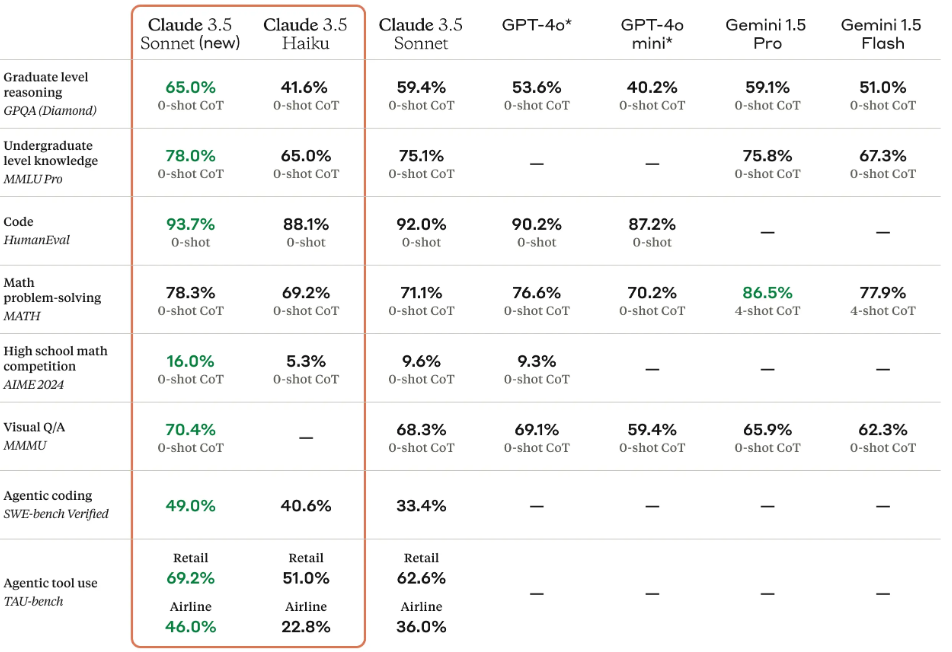
\includegraphics[scale=0.6]{sonnet-comparison.png}
    \caption{Confronto tra \textit{Sonnet} ed altri \gls{llm} - Ottobre 2024}
    \cite{site:updated-sonnet}
    \label{fig:sonnet-comparison}
\end{figure}
\pagebreak
\section{Codifica}
\label{sez:codifica}

\subsection{\textit{Best practices}}
\label{sez:best-practices}

Durante la fase di sviluppo del progetto ho adottato diverse \textit{best practices} di codifica, tra cui:

\begin{itemize}
    \item \textbf{\textit{Arrow Functions}}: Utilizzo consistente delle \textit{arrow functions} per una sintassi più concisa e un \textit{binding} più chiaro del \texttt{this}:
    \begin{verbatim}
    const add = (a, b) => a + b;
     \end{verbatim}
    \item \textbf{Convenzioni di \textit{naming}}: 
    \begin{itemize}
        \item \textit{PascalCase} per la definizione dei \textit{file ReactJs} e \textit{NestJs};
        \item \textit{camelCase} per variabili e funzioni;
        \item \textit{UPPER\_CASE} per le costanti.
    \end{itemize}

    \item \textbf{Creazione di un \textit{file .tsx} per ogni componente \textit{ReactJs}}:\\
    Questo approccio facilita i cambiamenti senza dover modificare il codice in più file. 
    Ogni componente \textit{ReactJs} ha il proprio \textit{file .tsx}, migliorando la modularità e la manutenibilità del codice.\\
    Ad esempio, un componente ‘\textit{SnackBar}‘ sarà definito in \textit{SnackBar.tsx}‘;
    
    \item \textbf{Utilizzo di \gls{git-flow}}: Struttura di \textit{branching} per una gestione più efficiente del ciclo di vita del software.\\
    Ampiamente discussa nella {\hyperref[subsec:vincoli-organizzativi]{Sezione 2.5.2}} relativa ai vincoli organizzativi;

    \item \textbf{\textit{Code Review}}: Ogni modifica al codice deve essere sottoposta a \textit{code review} da parte di un altro membro del \textit{team}.\\
    Questo processo aiuta a individuare errori, migliorare la qualità del codice e condividere conoscenze tra i membri del \textit{team};    
\end{itemize}


\subsection{\textit{Frontend}}
\label{sez:frontend}
Vado a descrivere la struttura dei file, i principali componenti e pagine create all'interno del frontend, come ad esempio la pagina di login, la dashboard, ecc.\\

\subsection{\textit{Backend}}
\label{sez:backend}

Vado a descrivere la struttura dei file, le principali API create, i collegamenti ai servizi AWS, ecc.\\
\pagebreak
\section{Verifica}
\label{sez:verifica}

La verifica è una fase cruciale del ciclo di vita del \textit{software}, finalizzata a garantire che il prodotto sviluppato soddisfi i requisiti specificati e sia privo di errori o difetti.\\
Questa attività si concentra sul controllo della correttezza, della completezza e della qualità del \textit{software}, sia a livello di codice che di comportamento.\\

\noindent La verifica può essere suddivisa in due approcci principali:

\begin{itemize}
\item \textbf{Analisi statica}:
È un processo che analizza il \textit{software} senza eseguirlo. \\
Si basa su tecniche di analisi statica, come le revisioni manuali del codice, l'uso di strumenti automatici per il controllo delle regole di codifica o per il \textit{linting} del codice. \\
Questo approccio consente di individuare errori, violazioni di standard, vulnerabilità e problemi di stile a livello di codice sorgente.  

\item \textbf{Analisi dinamica}:
Si basa sull’esecuzione del \textit{software} per testarne il comportamento in ambienti controllati o reali.\\
Questo approccio verifica che il sistema funzioni correttamente con \textit{input} specifici e che produca gli \textit{output} attesi. \\
Include attività come i \textit{test} unitari, \textit{test} di integrazione e \textit{test} di sistema.  
\end{itemize}

\noindent L’utilizzo combinato di analisi statica e dinamica è essenziale per garantire un livello elevato di qualità del \textit{software}. \\
Mentre l'analisi statica permette di affrontare i problemi a monte, l'analisi dinamica assicura che il sistema funzioni correttamente in condizioni operative. \\
Questo approccio integrato riduce al minimo il rischio di errori nel prodotto finale, migliorando l'affidabilità e la robustezza complessiva del \textit{software}.

\subsection{Analisi statica}
\label{subsec:analisi-statica}

Ho effettuato analisi statica per garantire che il codice sviluppato fosse conforme agli standard di qualità richiesti, riducendo la possibilità di errori e migliorandone la leggibilità e la manutenibilità.\\
Per questa attività ho utilizzato strumenti consolidati come \textit{Prettier} ed \textit{ESLint}, configurati per integrarsi con il flusso di lavoro del progetto.\\

\subsection{Analisi dinamica}
\label{subsec:analisi-dinamica}

Ho effettuato analisi dinamica per verificare il corretto funzionamento delle diverse componenti del sistema, con un particolare focus sul \gls{backend}, considerato il cuore del progetto, rispetto al \gls{frontend}, il cui \textit{testing} è stato affrontato solo in un secondo momento. \\
Le attività di \textit{testing} si sono concentrate prevalentemente sui \textit{test} unitari, con l'aggiunta di alcuni \textit{test} di performance per la generazione dei progetti.\\

\subsubsection{Testing del \gls{backend}}  

Ho sviluppato \textit{test} unitari per tutti i \textit{controller} ed i \textit{service}, assicurando la copertura di tutte le principali funzionalità del sistema.\\

\noindent I \textit{test} sono stati eseguiti durante tutto il ciclo di vita del \textit{software}, seguendo il modello a \textit{V} (visibile in {\hyperref[fig:v-model]{Figura 3.8}}), che prevede l’integrazione di attività di \textit{testing} in ogni fase di sviluppo.\\
    Man mano che venivano creati gli \textit{endpoint}, ho sviluppato i relativi \textit{test} per verificarne immediatamente la correttezza;

\noindent Questo approccio iterativo ha garantito che ogni componente fosse testata e verificata fin dalla sua creazione, riducendo al minimo la possibilità di accumulare errori e semplificando il \textit{debug} nelle fasi successive.\\

\begin{figure}[H]
    \centering
    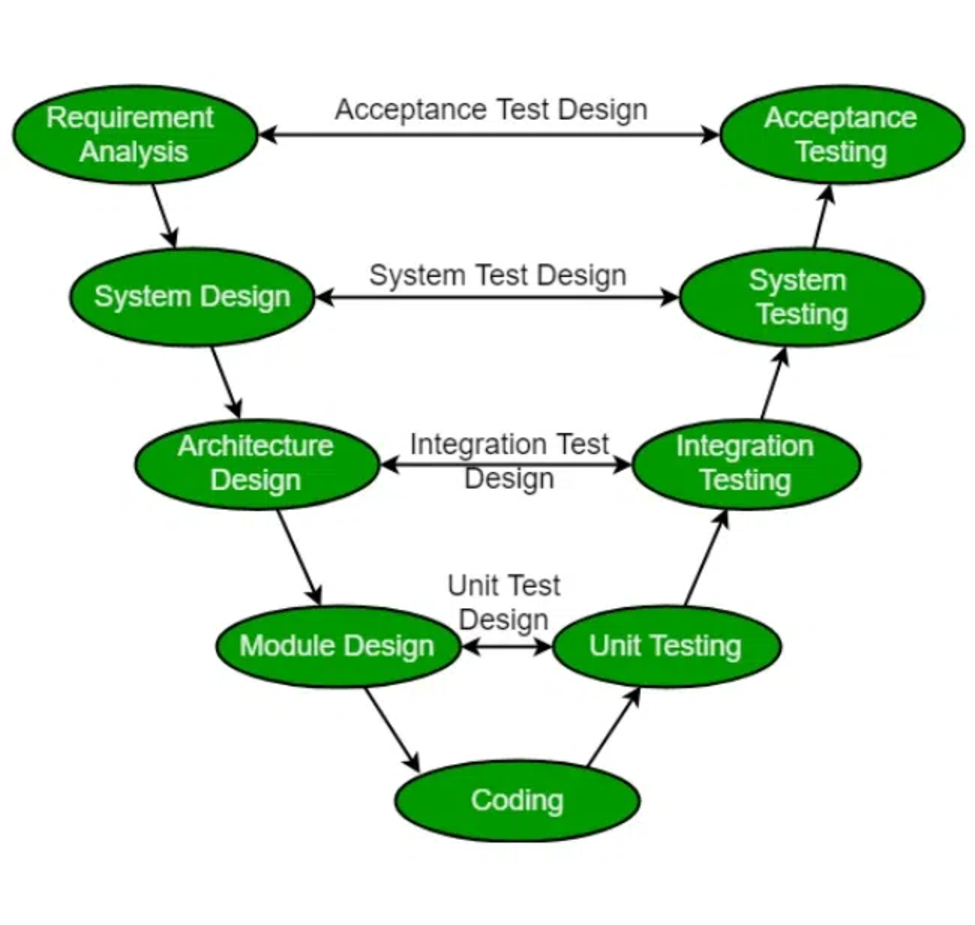
\includegraphics[scale=0.43]{v-model.png}
    \caption{Modello a V sviluppo \textit{software}}
    \label{fig:v-model}  
    \cite{site:v-model}
\end{figure}

\subsubsection{Test di performance}  
Ho effettuato alcuni \textit{test} di performance specifici per il \gls{backend}, con un focus particolare sulla generazione dei progetti.\\
Questi \textit{test} hanno permesso di misurare i tempi di risposta e verificare che il sistema fosse in grado di gestire la generazione di progetti in modo efficiente, anche in scenari di carico moderato.\\

\pagebreak
\section{Validazione}
\label{sez:validazione}

La validazione è il processo che verifica se il prodotto finale soddisfa i requisiti e le aspettative degli utenti o delle parti interessate. \\
A differenza della verifica, che si concentra sull’accuratezza e completezza tecnica delle singole componenti (ad esempio, controllando che il codice sia conforme alle specifiche), la validazione si focalizza sull’effettivo valore e utilità del \textit{software} nel contesto operativo previsto.  \\

\subsection{Test di accettazione}
\label{subsec:test-accettazione}

Ho condotto i \textit{test} di accettazione in collaborazione con il \textit{tutor} aziendale, con l’obiettivo di verificare che il progetto soddisfacesse i requisiti funzionali e non funzionali definiti in fase di analisi.\\

\noindent Durante la sessione di \textit{test}, il tutor aziendale ha valutato il comportamento del sistema rispetto alle aspettative aziendali e alle specifiche iniziali. La valutazione finale è stata positiva, confermando che il \textit{software} è pronto per essere utilizzato nell’ambiente di produzione e soddisfa pienamente le esigenze del progetto.
\subsection{Presentazione del progetto}
\label{subsec:presentazione-progetto}

L'ultima settimana di \textit{stage} mi è stata richiesta dall'azienda una presentazione finale del progetto ai colleghi aziendali, con l'obiettivo di illustrare il lavoro svolto, i problemi riscontrati durante lo sviluppo e le possibili migliorie da apportare in futuro.\\

\noindent Durante la presentazione ho spiegato lo scopo del progetto e le tecnologie utilizzate, evidenziando il valore aggiunto che potrebbe apportare all'azienda, ho inoltre mostrato una \textit{demo} del prodotto per dimostrare le sue funzionalità in tempo reale.\\  

\noindent La presentazione è stata accolta in modo molto positivo dai partecipanti. \\Al termine, sono state poste alcune domande per chiarire alcuni dettagli implementativi del progetto. In particolare, un collega ha manifestato interesse riguardo alla creazione dei \gls{prompt} utilizzati per la generazione dei progetti ed il loro processo di salvataggio, avviando un confronto costruttivo sull’argomento.\\
Questo ha confermato l’interesse e la rilevanza del lavoro svolto all'interno del contesto aziendale.


%\section{Risultati ottenuti}
\label{sez:risultati-ottenuti}


\subsection{Prodotto realizzato}
\label{subsec:prodotto-realizzato}

Screenshots del prodotto realizzato, spiegazione delle funzionalità implementate viste dal lato utente (in 'black-box').

\subsection{Copertura dei requisiti}
\label{subsec:copertura-requisiti}

Descrizione della copertura dei requisiti individuati durante l'analisi dei requisiti, quali sono stati soddisfatti, quali no, ecc.

\subsection{Materiali prodotti}
\label{subsec:materiali-prodotti}

Descrizione dei materiali prodotti durante il progetto, come il numero di linee di codice, numero di test implementati, il numero di documenti, il numero di file, ecc.\\

    \chapter{Retrospettiva finale}
\label{cap:retrospettiva-finale}

\section{Raggiungimento degli obiettivi}
\label{sez:raggiungimento-obiettivi}

\subsection{Obiettivi aziendali}
\label{subsec:raggiungimento-obiettivi-aziendali}

Riporto gli obiettivi aziendali indicati nella \hyperref[sez:obiettivi-aziendali]{Sezione §2.4} e descrivo se sono stati soddisfatti o meno alla fine dello stage.\\

\renewcommand{\arraystretch}{1.5} % Increases the row height for better vertical space

\begin{longtable}{|c|>{\centering\arraybackslash}p{0.7\textwidth}|c|} % Adjust the column width with p{0.7\textwidth}
    \hline
    \rowcolor{green!30} % Header color: light green
    \textbf{Codice Obiettivo} & \textbf{Descrizione Obiettivo} & \textbf{Soddisfatto}\\
    \hline
    \endfirsthead % Start of the table, first header
    
    \hline
    \rowcolor{green!30} % Header color on subsequent pages
    \textbf{Codice Obiettivo} & \textbf{Descrizione Obiettivo} & \textbf{Soddisfatto}\\
    \hline
    \endhead % Continuation of the table (repeats on every page)
    
    \hline
    \multicolumn{3}{|c|}{\rowcolor{green!30} \textbf{Obiettivi Obbligatori}}  \\
    \hline % Adds a horizontal line after the header row
    \textbf{OO-1} & \textbf{Apprendimento delle tecnologie di sviluppo:} Acquisire competenze pratiche nell'uso di \textit{React}, \textit{NestJS} e \textit{MongoDB} per la progettazione e lo sviluppo di applicazioni. & SI \\

    \hline
    \textbf{OO-2} & \textbf{Gestione del versionamento del codice:} Apprendere l'uso di \textit{Git} e adottare \textit{Git Flow} come metodologia per il controllo delle versioni e la collaborazione. & SI\\
    \hline
    \textbf{OO-3} & \textbf{Analisi e scelta del \gls{llm}:} Valutare i modelli disponibili per selezionare quello più adatto al progetto.& SI \\
    \hline
    \textbf{OO-4} & \textbf{Introduzione alle metodologie agili:} Familiarizzare con le metodologie agili di sviluppo per la gestione efficace di progetti. & SI\\
    \hline
    \textbf{OO-5} & \textbf{Pianificazione e gestione giornaliera:} Imparare a gestire \textit{task} e obiettivi giornalieri allineati al piano di lavoro. & SI\\
    \hline
    \textbf{OO-6} & \textbf{Sviluppo di una \textit{web app:}} Progettare e realizzare un'applicazione \textit{web} per consentire l'interazione dell'utente con la piattaforma. & SI\\
    \hline
    \textbf{OO-7} & \textbf{Sviluppo ed integrazione con \gls{generative-ai}:} Implementare i flussi logici del progetto e integrare i servizi di \gls{generative-ai} scelti. & SI\\
    \hline
    \textbf{OO-8} & \textbf{Documentazione \gls{api}:} Creare una documentazione \textit{Swagger} per le \gls{api} sviluppate.& SI \\
    \hline
    \textbf{OO-9} & \textbf{Documento di analisi progettuale:} Redigere un documento tecnico che descriva l'architettura e le componenti principali della piattaforma.& SI \\
    \hline
    \textbf{OO-10} & \textbf{\textit{User Story Mapping:}} Realizzare una mappatura delle \gls{user-stories} per descrivere e organizzare i requisiti del progetto.& SI \\
    \hline
    \multicolumn{3}{|c|}{\rowcolor{green!30} \textbf{Obiettivi Desiderabili}} \\
    \hline % Adds a horizontal line after the subtitle
    \textbf{OD-1} & \textbf{Comparazione tra modelli \gls{llm}:} Effettuare un'analisi comparativa tra almeno due \gls{llm} per verificarne le differenze in termini di prestazioni, funzionalità e costi.& NO \\
    \hline
    \multicolumn{3}{|c|}{\rowcolor{green!30} \textbf{Obiettivi Facoltativi}} \\
    \hline % Adds a horizontal line after the subtitle
    \textbf{OF-1} & \textbf{Piattaforma di amministrazione:} Creare una piattaforma \textit{admin} per la gestione dei \textit{Preset} e dei modelli \gls{llm}.& NO \\
    \hline
    \caption{Obiettivi aziendali dello \textit{stage}} % Table caption
    \label{tab:raggiungimento_obiettivi_stage} % Label for referencing the table
\end{longtable}

\noindent Sono riuscito a soddisfare il 100\% degli obiettivi obbligatori del progetto, garantendo il raggiungimento di tutte le funzionalità essenziali. \\
Tuttavia, non sono riuscito a completare nessuno degli obiettivi desiderabili o facoltativi, a causa di limitazioni tecniche e di tempo.\\

\noindent In particolare, non ho raggiunto l'obiettivo OD-1 (Comparazione tra modelli \gls{llm}) a causa della complessità tecnica nell'integrare diversi modelli con \textit{AWS Bedrock} e nell'effettuare un'analisi approfondita delle loro prestazioni.\\
Inoltre, il tempo a disposizione non è stato sufficiente per completare le configurazioni necessarie.\\

\noindent Allo stesso modo, non sono riuscito a completare lo sviluppo della piattaforma di amministrazione (OF-1).
Questo obiettivo, essendo secondario rispetto alle priorità principali del progetto, non ha potuto ricevere l’attenzione necessaria entro i tempi disponibili.
\pagebreak
\subsection{Obiettivi personali}
\label{subsec:raggiungimento-obiettivi-personali}

Riporto gli obiettivi personali indicati nella \hyperref[sez:obiettivi-personali]{Sezione §2.6} e descrivo se sono stati soddisfatti o meno alla fine dello stage.\\

\renewcommand{\arraystretch}{1.5} % Increases the row height for better vertical space

\begin{longtable}{|c|>{\centering\arraybackslash}p{0.7\textwidth}|c|} % Adjust the column width with p{0.7\textwidth}
    \hline
    \rowcolor{green!30} % Header color: light green
    \textbf{Codice Obiettivo} & \textbf{Descrizione Obiettivo} & \textbf{Soddisfatto}\\
    \hline
    \endfirsthead % Start of the table, first header
    
    \hline
    \rowcolor{green!30} % Header color on subsequent pages
    \textbf{Codice Obiettivo} & \textbf{Descrizione Obiettivo}  & \textbf{Soddisfatto}\\
    \hline
    \endhead % Continuation of the table (repeats on every page)
    
    \hline
    \multicolumn{3}{|c|}{\rowcolor{green!30} \textbf{Obiettivi Personali}} \\
    \hline
    \textbf{OP-1} & \textbf{Padroneggiare nuovi linguaggi e \textit{framework}:} Acquisire competenze avanzate nello sviluppo di applicazioni utilizzando \textit{React} per il \gls{frontend} e \textit{NestJS} per il \gls{backend}, implementando progetti reali che sfruttano queste tecnologie. & SI \\
    \hline
    \textbf{OP-2} & \textbf{Esplorare i servizi \textit{cloud} di \gls{aws}:} Imparare ad utilizzare servizi come \textit{AWS Amplify}, \textit{AWS Cognito}, \textit{AWS S3}, e \textit{AWS Bedrock}, comprendendo come integrarli in un’architettura scalabile e moderna. & SI\\
    \hline
    \textbf{OP-3} & \textbf{Competenze in \gls{generative-ai}:} Sviluppare un solido \textit{know-how} nell’utilizzo di tecnologie di \gls{generative-ai}, come l’integrazione di modelli \textit{AI (Claude, GPT)} in progetti pratici.& SI \\
    \hline
    \multicolumn{3}{|c|}{\rowcolor{green!30} \textbf{Obiettivi di Crescita Personale}} \\
    \hline
    \textbf{OP-4} & \textbf{Comprendere il settore professionale:} Ottenere una visione del contesto aziendale del settore tecnologico, analizzando flussi di lavoro e \textit{trend} di mercato, per orientare al meglio il percorso professionale futuro.& SI \\
    \hline
    \textbf{OP-5} & \textbf{Ottimizzare la gestione del tempo:} Sviluppare un approccio strutturato al lavoro, utilizzando strumenti di produttività e tecniche di prioritizzazione per rispettare scadenze e migliorare l’efficienza personale. & SI\\
    \hline
    \textbf{OP-6} & \textbf{Comunicazione professionale efficace:} Rafforzare le capacità di comunicazione scritta e orale per facilitare il dialogo e le collaborazioni.& SI \\
    \hline
    \multicolumn{3}{|c|}{\rowcolor{green!30} \textbf{Obiettivi di Autonomia e Collaborazione}} \\
    \hline
    \textbf{OP-7} & \textbf{Lavoro indipendente:} Incrementare la capacità di gestire \textit{task} e progetti in modo autonomo, prendendo decisioni informate e risolvendo problemi complessi senza supervisione diretta.& SI \\
    \hline
    \textbf{OP-8} & \textbf{Collaborazione proattiva:} Contribuire attivamente al lavoro di squadra, partecipando a \textit{meeting}, condividendo idee e accogliendo \textit{feedback} per migliorare continuamente le proprie performance. & Parzialmente\\
    \hline
    \caption{Obiettivi personali dello \textit{stage}} % Table caption
    \label{tab:raggiungimento-obiettivi-personali-stage} % Label for referencing the table
\end{longtable}

\noindent Ho raggiunto tutti i miei obiettivi personali, ad eccezione dell'obiettivo OP-8 (Collaborazione proattiva), che sono riuscito a soddisfare solo in parte.\\

\noindent In particolare, il mio obiettivo di contribuire attivamente al lavoro di squadra, partecipando a \textit{meeting}, condividendo idee e accogliendo \textit{feedback}, non è stato pienamente raggiunto.\\
Anche se ho preso parte a diversi \textit{meeting}, ho lavorato principalmente in autonomia e non ho avuto molte opportunità di collaborare attivamente con un \textit{team}.
\input{chapters/retrospettivaFinale/difficoltà-incontrate.tex}
\section{Crescita professionale}
\label{sez:crescita-professionale}

\input{chapters/retrospettivaFinale/difficoltà-incontrate.tex}

\pagebreak
\subsection{Competenze acquisite}
Nel corso del progetto ho sviluppato e perfezionato diverse competenze, che possono essere suddivise in tre categorie principali:

\begin{itemize}
\item \textbf{Competenze tecniche}:
Ho approfondito e migliorato significativamente la mia conoscenza di \textit{TypeScript}, applicandolo con successo in un progetto complesso nel contesto dello sviluppo \textit{web}. \\
Ho inoltre acquisito competenze nell'utilizzo di diversi servizi \gls{aws}, con un focus particolare su \textit{AWS Bedrock}, dedicato alla \gls{generative-ai}.\\
Questo mi ha permesso di affrontare aspetti tecnici avanzati e di integrare nuove tecnologie nel progetto in maniera efficace;
\item \textbf{Competenze metodologiche}:  
Ho avuto modo di lavorare seguendo un approccio \textit{agile}, partecipando attivamente agli \gls{sprint} e rispettandone le tempistiche. \\  
Inoltre, ho affinato la mia capacità di organizzazione autonoma, definendo con precisione le priorità e gestendo le attività necessarie per portare a termine il lavoro in modo efficiente;

\item \textbf{Competenze personali}:  
Grazie alla partecipazione alle \textit{sprint review} e alla presentazione aziendale del progetto, ho migliorato le mie competenze comunicative, imparando a esporre il mio lavoro in maniera chiara, strutturata e professionale. \\  
Ho anche sviluppato ulteriormente le mie capacità di \textit{problem solving}, trovando soluzioni creative e pratiche alle difficoltà incontrate durante le diverse attività del progetto.  
\end{itemize}
\section{Università e mondo del lavoro}
\label{sez:universita-mondo-lavoro}

Connessioni e differenze tra il mondo dell'università e il mondo del lavoro.\\
Come l'università mi abbia preparato per il mondo del lavoro, ecc.\\

\pagebreak
\section{Considerazioni finali}
\label{sec:considetazioni-finali}

Ritengo l’esperienza di \textit{stage} presso \textit{Zero12} estremamente positiva, sia per l’argomento trattato sia per il risultato raggiunto.\\
In particolare, lavorare su un tema innovativo e di grande rilevanza come la \gls{generative-ai}, combinato con l’utilizzo dei servizi \gls{aws}, mi ha permesso di acquisire competenze tecniche avanzate e di esplorare tecnologie all’avanguardia. \\ 

\noindent Sono riuscito a creare un progetto completo, che ha superato le mie stesse aspettative.\\
Questo risultato non solo mi ha dato grande soddisfazione personale, ma ha anche consolidato la mia fiducia nelle mie capacità di affrontare sfide complesse e di portare a termine attività ambiziose.\\  

\noindent L’ambiente di lavoro di \textit{Zero12} è stato un elemento chiave per il successo di questa esperienza.\\
Ho trovato un contesto altamente stimolante, caratterizzato da un elevato livello di professionalità e da una cultura aziendale orientata all’innovazione e alla sperimentazione.\\
La disponibilità e il supporto dei colleghi, uniti a una costante attenzione alla formazione e al miglioramento, hanno reso questo percorso formativo non solo proficuo, ma anche particolarmente gratificante. \\

\noindent In conclusione, considero questo \textit{stage} un’esperienza fondamentale per la mia crescita personale e professionale, che ha arricchito il mio bagaglio di conoscenze e mi ha fornito strumenti preziosi per il futuro.

    %\appendix
    %\chapter{Appendice A}

\epigraph{Citazione}{Autore della citazione}


    \backmatter
    \printglossary[type=\acronymtype, title=Acronimi e abbreviazioni, toctitle=Acronimi e abbreviazioni]
    \printglossary[type=main, title=Glossario, toctitle=Glossario]

    \cleardoublepage
\chapter{Bibliografia}

\nocite{*}

% Print book bibliography
\printbibliography[heading=subbibliography,title={Riferimenti bibliografici},type=book]

% Print site bibliography
\printbibliography[heading=subbibliography,title={Siti web consultati},type=online]

\end{document}
